\documentclass{book}
\usepackage[UTF8]{ctex}
\usepackage{amsmath,mathtools,geometry,pgfplots,float,mathrsfs,caption,enumerate,paracol,yhmath,color,fancyhdr,framed}
\usepackage{tcolorbox}
\usepackage[center]{titlesec}
\usepackage[strict]{changepage}
\usetikzlibrary{patterns}

\geometry{a4paper, scale=0.85}

\pagestyle{fancy}
\fancyhead[EL]{

\begin{tikzpicture}
	\fill [color=cyan!70] (0,0) circle (0.3);
	\fill [color=cyan!50] (0.6,0) circle (0.3);
	\fill [color=cyan!30] (1.2,0) circle (0.3);
	\node at (0,0) {\textbf{\thepage}};
\end{tikzpicture}
}
\fancyhead[OL]{\slshape \rightmark}
\fancyhead[OR]{

\begin{tikzpicture}
	\fill [color=cyan!70] (0,0) circle (0.3);
	\fill [color=cyan!50] (-0.6,0) circle (0.3);
	\fill [color=cyan!30] (-1.2,0) circle (0.3);
	\node at (0,0) {\textbf{\thepage}};
\end{tikzpicture}
}
\fancyfoot[C]{}

\footnotelayout{m}

\captionsetup[figure]{labelfont=it}

\pgfplotsset{compat=1.15}
\usetikzlibrary{arrows}

\columnratio{0.73}           
\setlength{\columnsep}{1em}  
\twosided[pc]

\setlength{\parsep}{0pt}
\setlength{\itemsep}{0pt}

\titleformat{\chapter}{\raggedright\Huge\bfseries}{{\rm\huge\kaishu\textit{第\,\thechapter\ 章}}}{1em}{\\}
\titleformat{\section}{\centering\Large\bfseries\color{cyan!60!blue}}{\color{cyan!60!blue}\Large\textbf{\thesection}}{1em}{}
\titleformat{\subsection}{\raggedright\large\bfseries}{\large\textbf{\thesubsection}}{1em}{}

\newenvironment{theorem}{%
\def\FrameCommand{%
\hspace{1pt}%
{\color{cyan!60!blue}\vrule width 2pt}%
{\color{cyan!10}\vrule width 4pt}%
\colorbox{cyan!10}%
}%
\MakeFramed{\advance\hsize-\width\FrameRestore}%
\noindent\hspace{-4.55pt}% disable indenting first paragraph
\begin{adjustwidth}{}{7pt}%
\vspace{2pt}\vspace{2pt}%
}
{%
\vspace{2pt}\end{adjustwidth}\endMakeFramed%
}


\title{\textbf{\heiti{几何专题}}}
\author{\kaishu 程昊一}
\date{2023年1月}

\begin{document}
\backgroundcolor{c[1]}[rgb]{0.95,1,1}
\tcbset{colframe=cyan,colback=cyan!10,
	bottomrule=-0.01mm,rightrule=-0.01mm,
	arc is angular,arc=4mm,outer arc=0mm,sharp corners=uphill}
\maketitle\newpage
\thispagestyle{plain}

\vspace*{2.25cm}
{\raggedright\Huge\bfseries{前言}}
\vspace*{1cm}\par 
本章就如何解平面几何问题做一些探讨与说明.\par
首先, 我们要说明一点: \textbf{熟悉与掌握基本图形与结构是正确迅速解决平面几何问题的重要前提}. 我经常有这样的感受: 翻阅以前写过的当时认为的“难题”, 发现如果以现在的眼光去看, 那么结论的证明几乎是显然的. 为什么为由如此之大的差异? 那就是相较于之前, 现在我对这道题所涉及的结构有了更深的理解. 例如, 在小蓝本初中卷的第五本《圆》中, 就有我一年多前未解决的题, 但现在看来, 只是对某个基本结构的加工与改造, 或是几何基本结构的合成. 之所以当时没有解出这些题, 就是因为当时对于这些结构的了解不够深刻、熟悉程度不够. 由此可见, 熟悉与掌握基本图形与结构是非常有必要的.\par
在一本以平面几何为主要内容的数学竞赛书\footnote{沈文选, 杨清桃. 高中数学竞赛解题策略(几何分册)[M]. 杭州: 浙江大学出版社, 2012.}的前言中, 对此有较为详细的描述, 如下:
\begin{quote}
	\kaishu \hspace{2em}一个人在解决平面几何问题中体现出来的能力, 其实质是根据问题情景重组已知的平面几何图形知识, 能正确、迅速地检索、选择和提取相关平面几何图形知识并及时转化为适当的操作程序, 从而将问题从初始状态转变为目的状态. 丰富、系统的平面几何图形知识不仅是解题创新所不可或缺的材料, 而且还能直接激发解题创新的直觉或灵感. 只有具备了充分的几何图形与逻辑推理知识, 才有可能进行有目的、有方向、有成效的探究性活动, 求解数学竞赛中的几何问题效能才有保障, 否则就只能是尝试错误. 因此, 为了在各级各类数学竞赛中取得好的成绩, 应该以几何图形为手段, 以基本图形性质为核心, 逐步认识基本图形为目标来进行学习. 认识基本图形, 深入挖掘特性, 善用平台析题, 思路快捷清晰. 
\end{quote}\par
那么, 对于大家来说, 这些道理仍然是适用的. 熟悉基本图形, 是快速解题的必要条件.\par
那么, 如何做到熟悉与掌握基本图形与结构?\par
我们仍然强调要多思考. 机械地整理与记录对此是几乎没有什么帮助的. 对于老师上课讲到的或是作业中的题, 要积极思考其中所蕴含的结构. 并且, 可以尝试提炼各个题之间所蕴含的共同的图形与结构. 如果某个结构出现的频率非常高, 那么这个结构就是必须要好好研究与掌握的. 并且, 老师布置的整理作业也是必要的. 有时候, 几何结构可能太多而无法一次记住(正如俗语“一口吃不成个胖子”), 便很有必要用一个本子来记录. 当然, 我们再次强调, 这里的记录绝不是不加思考的抄写.\par 
另外, 知识之间的联系也是很重要的. 搭建一个清晰有序的知识框架是很有必要的, 这样才能在解题时迅速找到所需要的知识与几何结构. 否则, 所有的知识搅和在一起, 解题的时候可能就会出现没有思路, 即无法找到对应的几何结构; 或是有了太多的思路, 只要有一点点联系就能想到, 而无法根据题目本身的特点找到对应的最合适的知识, 这样也是不利于解题的.\par
有时候, 某些解题的思想也是比较重要的. 这一点可能对于大多数同学比较抽象. 例如, 对于点的“刻画”, 对于找到思路、利用条件是很有帮助的. 再比如, 让图形“运动起来”, 对于某些知识的理解也是有益的. 我们将会在后面详细介绍. 当然, 对于中考或中考拔高的几何问题, 它们的难度还不足以体现这些思想的重要性, 如果同学们多做些难题, 肯定会有相同的感受.\par
我们还必须要强调一点, 就是关于三角法与解析法(即俗称的“建系”)的使用. 这两种方法的特点均为以较大的计算量代替较难的几何思考过程(但这并不说明计算的方法是完全没有思考量的). 固然, 某些题目运用这些方法来解决是直截了当的, 但我们必须强调的一点是: 在\textbf{平日的训练几何思维能力}时, 尽量不要使用计算量大而思考复杂程度小的方法. 甚至, 某些难题不能轻松使用计算的方法算出, 否则将面临难以想象的计算量. 为什么要强调这一点? 这是因为计算的方法对于几何思维能力的提升的效果甚微. 固然, 对于某些难题, 计算也是有技巧的, 但如果想训练几何思维能力, 那么请尽量想出纯几何的方法, 而不是完全是三角法或解析法. 当然, \textbf{在考场上}, 我们永远要选择最利于得到分数的方法解题. 此时, 利于得分的方法便是好方法(“不管黑猫白猫,抓住老鼠就是好猫”).\par
在这篇文档中, 我们将会介绍基本的圆的知识、三角形的五心与若干特殊的几何结构. 这之中, 有的是基础知识(如第一章的大部分), 有的是在题目中经常出现的, 有的是可以作为兴趣了解的. 希望这篇文档能够帮助大家学习到更多的知识, 同时对于平面几何与平面几何解题的理解更进一步.




\chapter{四点共圆与圆幂定理}
\thispagestyle{empty}

圆可谓是平面几何中最丰富的图形, 许多几何构型与结论都直接与圆有关系. 可以说, 圆极大地丰富了平面几何的内容. 下面我们就来了解一下圆的基本性质,和平面几何中一个极其重要的概念———四点共圆.

\section{圆的定义与性质}

\begin{paracol}{2}

大家一定都很清楚圆的定义: \textbf{圆}是平面内到一定点距离为定长的点的集合.	下面我们来探究一下圆的性质.\par
想要研究它的性质, 我们能用的只有圆的定义和其他已经证明的定理.\par
在此之前, 我们先定义一些名词:
\begin{enumerate}[(1)]
	\item\textbf{圆心}\quad 定义中的“定点”;
	\item\textbf{半径}\quad 定义中的“定长”, 或指一端为圆心, 另一端在圆上的一条线段;
	\item\textbf{直径}\quad 半径的2倍, 或指两端在圆上且过圆心的一条线段;
	\item\textbf{圆弧}\quad 圆上任意两点之间的部分, 简称“弧”, 其中较长的称为“优弧”, 较短的称为“劣弧”; 
	\item\textbf{弦}\quad 两端均在圆上的线段;
	\item\textbf{圆心角}\quad 在以$O$为圆心的圆中, 过弧$AB$端点的两条半径所构成的角, 此圆心角经常被称为“弧$AB$所对的圆心角”;
	\item\textbf{圆周角}\quad 顶点$P$在圆上, 且两条边均与圆相交(不妨设为$A$与$B$)的角, 此圆周角经常被称为“弧$AB$所对的圆周角”.
\end{enumerate}\par
由图\ref{fig:yuan_zhou_jiao}不难知道, \textbf{同弧所对的圆心角是圆周角的2倍.} 当然, 此图只是 $O$ 在 $\angle ACB$ 内的情况,对于$O$在$\angle ACB$边上或者外部的情况, 与在内部的情况类似. 将上述定理中的“同弧”换为“等弧”(即所对圆心角相等的弧), 也是正确的.\par
并且, 我们会发现, 对于圆周角$\angle ACB$与$\angle ADB$($C$与$D$在点$A$与$B$所划分的同一个弧内), 设圆心为$O$, 那么我们有
\[\angle ACB=\frac{1}{2}\angle AOB=\angle ADB.\]
而且, 我们可以在同一条弧内任取$C$与$D$, 总有$\angle ACB=\angle ADB$, 所以, 对于此弧上的的任意一点$P$, $\angle APB$为定值. 即,\textbf{同弧(或等弧)所对圆周角相等}. 这个定理极为重要, 用途极为广泛. \par
\switchcolumn
\begin{figure}[htbp]
	\centering
	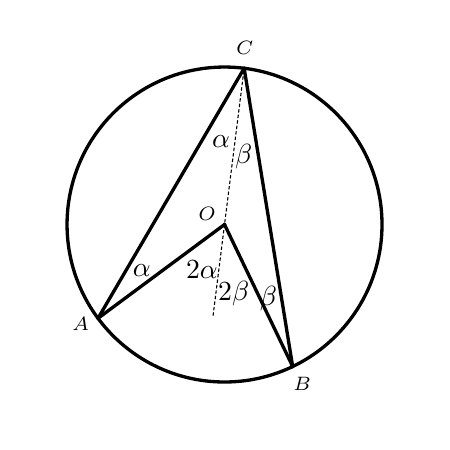
\begin{tikzpicture}[line cap=round,line join=round,>=triangle 45,x=1cm,y=1cm]
		\clip(-2.5,-2.5) rectangle (2.5,2.5);
		\draw [line width=1.2pt] (0.,0.) circle (2);
		\draw [line width=1.2pt] (0.24947738920300175,1.9843792561595814)--(-1.606614939932181,-1.1911290588289392);
		\draw [line width=1.2pt] (0.8653514034999357,-1.8030992619544526)--(0.24947738920300175,1.9843792561595814);
		\draw [line width=1.2pt] (0.,0.)-- (-1.606614939932181,-1.1911290588289392);
		\draw [line width=1.2pt] (0.8653514034999357,-1.8030992619544526)-- (0.,0.);
		\draw [line width=0.4pt,dash pattern=on 1pt off 1pt](-0.14521197670299205,-1.155037076650146)-- (0.24947738920300175,1.9843792561595814);
		\draw (-0.2816448244594834,1.2520397816187543) node[anchor=north west] {$\alpha$};
		\draw (-1.2896117069314856,-0.37917379917562655) node[anchor=north west] {$\alpha$};
		\draw (-0.6125041828281559,-0.3330073770776724) node[anchor=north west] {$2\alpha$};
		\draw (0.010742515494227172,1.1443181300568612) node[anchor=north west] {$\beta$};
		\draw (0.3262130664969149,-0.663866735446344) node[anchor=north west] {$\beta$};
		\draw (-0.20470078762955957,-0.602311505982405) node[anchor=north west] {$2\beta$};
		\begin{scriptsize}
			\draw [fill=black] (0.,0.) circle (0.5pt);
			\draw[color=black] (-0.22008959499554434,0.1401984494263579) node {$O$};
			\draw [fill=black] (-1.606614939932181,-1.1911290588289392) circle (0.5pt);
			\draw[color=black] (-1.8282199647409525,-1.2678774245612443) node {$A$};
			\draw [fill=black] (0.8653514034999357,-1.8030992619544526) circle (0.5pt);
			\draw[color=black] (0.9879317832342599,-2.0296233891774884) node {$B$};
			\draw [fill=black] (0.24947738920300175,1.9843792561595814) circle (0.5pt);
			\draw[color=black] (0.25696343334998345,2.240770654883273) node {$C$};
		\end{scriptsize}
	\end{tikzpicture}
	\caption{}\label{fig:yuan_zhou_jiao}
\end{figure}
\switchcolumn*
如图\ref{fig:yuan_zhou_jiao_const}, 点$P$在优弧$\wideparen{AB}$上, 则$\angle APB$为定值.\par
还有一件事情值得注意:\par
如图, 在优弧$\wideparen{AB}$上有一点$P$, 劣弧$\wideparen{AB}$上有一点$Q$. 那么,
\[\angle APB=\frac{1}{2}\text{劣弧}AB\text{所对圆心角};\]
\[\angle AQB=\frac{1}{2}\text{优弧}AB\text{所对圆心角}.\]
而两个弧加起来刚好是一个圆周, 所以两个弧的圆心角相加为$360^\circ$. 由此得到
\[\angle APB+\angle AQB=180^\circ.\]\par
这条定理与上一条定理同样重要, 几乎所有的圆的结论都是由这两个定理推出的.
\switchcolumn
\begin{figure}[htbp]
	\centering
	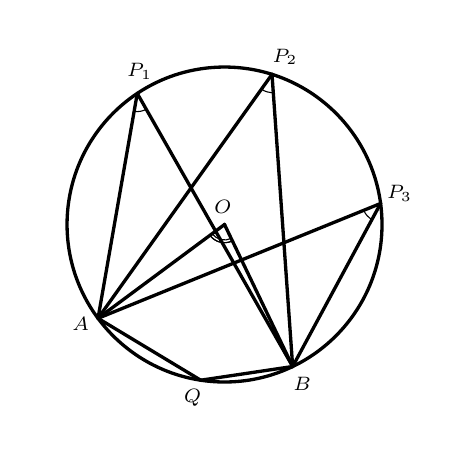
\begin{tikzpicture}[line cap=round,line join=round,>=triangle 45,x=1.0cm,y=1.0cm]
		\clip(-2.5,-2.5) rectangle (2.5,2.5);
		\draw [shift={(-1.1082779283861117,1.664848351487963)},line width=0.4pt] (0,0) --(-99.89784208781442:0.23083211048977154) arc(-99.89784208781442:-60.35554181697558:0.23083211048977154) -- cycle;
		\draw [shift={(0.602973444412513,1.9069407503468245)},line width=0.4pt] (0,0) --(-125.49701720684968:0.23083211048977154) arc(-125.49701720684968:-85.95471693601083:0.23083211048977154) -- cycle;
		\draw [shift={(1.982040597858693,0.26742301404320923)},line width=0.4pt] (0,0) --(-157.8814971107945:0.23083211048977154) arc(-157.8814971107945:-118.33919683995563:0.23083211048977154) -- cycle;
		\draw [shift={(0.,0.)},line width=0.4pt] (0,0) --(-143.44711340930624:0.23083211048977154)arc (-143.44711340930624:-64.36251286762854:0.23083211048977154) -- cycle;
		\draw [line width=1.2pt] (0.,0.) circle (2.cm);
		\draw [line width=1.2pt] (-1.1082779283861117,1.664848351487963)--(-1.606614939932181,-1.1911290588289392);
		\draw [line width=1.2pt] (0.8653514034999357,-1.8030992619544526)--(-1.1082779283861117,1.664848351487963);
		\draw [line width=1.2pt] (0.,0.)-- (-1.606614939932181,-1.1911290588289392);
		\draw [line width=1.2pt] (0.8653514034999357,-1.8030992619544526)-- (0.,0.);
		\draw [line width=1.2pt] (-1.606614939932181,-1.1911290588289392)--(0.602973444412513,1.9069407503468245);
		\draw [line width=1.2pt] (0.602973444412513,1.9069407503468245)--(0.8653514034999357,-1.8030992619544526);
		\draw [line width=1.2pt] (-1.606614939932181,-1.1911290588289392)--(1.982040597858693,0.26742301404320923);
		\draw [line width=1.2pt] (1.982040597858693,0.26742301404320923)--(0.8653514034999357,-1.8030992619544526);
		\draw [shift={(0.,0.)},line width=0.4pt] (-143.44711340930624:0.23083211048977154) arc(-143.44711340930624:-64.36251286762854:0.23083211048977154);
		\draw [shift={(0.,0.)},line width=0.4pt] (-143.44711340930624:0.1962072939163058) arc(-143.44711340930624:-64.36251286762854:0.1962072939163058);
		\draw [line width=1.2pt] (-0.3019893875281549,-1.9770691464438894)--(-1.606614939932181,-1.1911290588289392);
		\draw [line width=1.2pt] (-0.3019893875281549,-1.9770691464438894)--(0.8653514034999357,-1.8030992619544526);
		\begin{scriptsize}
			\draw [fill=black] (0.,0.) circle (0.5pt);
			\draw[color=black] (-0.020035099237740616,0.22483688993927298) node {$O$};
			\draw [fill=black] (-1.606614939932181,-1.1911290588289392) circle (0.5pt);
			\draw[color=black] (-1.8282199647409507,-1.2678774245612452) node {$A$};
			\draw [fill=black] (0.8653514034999357,-1.8030992619544526) circle (0.5pt);
			\draw[color=black] (0.9879317832342617,-2.0296233891774893) node {$B$};
			\draw [fill=black] (-1.1082779283861117,1.664848351487963) circle (0.5pt);
			\draw[color=black] (-1.0780156056491934,1.9445361130880658) node {$P_1$};
			\draw [fill=black] (0.602973444412513,1.9069407503468245) circle (0.5pt);
			\draw[color=black] (0.7686412782689787,2.1292018014798826) node {$P_2$};
			\draw [fill=black] (1.982040597858693,0.26742301404320923) circle (0.5pt);
			\draw[color=black] (2.222883574354539,0.39796097280660114) node {$P_3$};
			\draw [fill=black] (-0.3019893875281549,-1.9770691464438894) circle (0.5pt);
			\draw[color=black] (-0.40475528338735983,-2.198900270203321) node {$Q$};
		\end{scriptsize}
	\end{tikzpicture}
	\caption{}\label{fig:yuan_zhou_jiao_const}
\end{figure}
\switchcolumn*
下面我们再介绍一条定理, 即\textbf{垂径定理}. 它很好地反应了圆的对称性.
\begin{theorem}
	\textbf{垂径定理}\quad {\kaishu
	如图\ref{fig:chui_jing}, 在$\odot O$中, 有两条弦$AB$, $CD$相交. 那么, 下面五个命题中, 任选2个作为条件, 其余作为结论, 除了(3)(5)不能证出(1)(2)(4)外, 均为真命题:\begin{enumerate}[(1)]
		\item 弦$CD$平分弦$AB$所对的优弧;
		\item 弦$CD$平分弦$AB$所对的劣弧;
		\item 弦$CD$平分弦$AB$; 
		\item 弦$CD$垂直于弦$AB$;
		\item 弦$CD$过圆心$O$.
	\end{enumerate} 
	}
\end{theorem}

事实上, 这个定理包含9个命题, 证明均不困难, 留给大家完成. 大多数命题都主要考虑的是两个三角形: $\triangle APO$与$\triangle BPO$.
需要注意的是, 可能有同学不知道“弦平分弧”的含义是什么.\par
例如, “弦$CD$平分弦$AB$所对的优弧”, 就是点$C$平分优弧$\wideparen{AB}$, 这意味着 $\wideparen{AC}$ 与$\wideparen{CB}$ 为等弧, 即$\angle AOC=\angle COB$.

\switchcolumn
\begin{figure}[htbp]
	\centering
	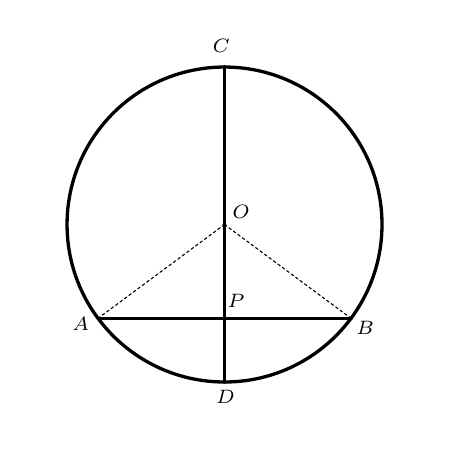
\begin{tikzpicture}[line cap=round,line join=round,>=triangle 45,x=1.0cm,y=1.0cm]
		\clip(-2.5,-2.5) rectangle (2.5,2.5);
		\draw [line width=1.2pt] (0.,0.) circle (2.cm);
		\draw [line width=0.4pt,dash pattern=on 1pt off 1pt] (0.,0.)--(-1.606614939932181,-1.1911290588289392);
		\draw [line width=1.2pt] (1.6066149399321812,-1.1911290588289392)--(-1.606614939932181,-1.1911290588289392);
		\draw [line width=1.2pt] (0.,2.)-- (0.,-2.);
		\draw [line width=0.4pt,dash pattern=on 1pt off 1pt] (0.,0.)--(1.6066149399321812,-1.1911290588289392);
		\begin{scriptsize}
			\draw [fill=black] (0.,0.) circle (0.5pt);
			\draw[color=black] (0.2107970112520309,0.15558725679234173) node {$O$};
			\draw [fill=black] (-1.606614939932181,-1.1911290588289392) circle (0.5pt);
			\draw[color=black] (-1.8282199647409507,-1.2678774245612452) node {$A$};
			\draw [fill=black] (1.6066149399321812,-1.1911290588289392) circle (0.5pt);
			\draw[color=black] (1.7881497662654695,-1.306349442976207) node {$B$};
			\draw [fill=black] (0.,2.) circle (0.5pt);
			\draw[color=black] (-0.04311831028671777,2.2715482696152414) node {$C$};
			\draw [fill=black] (0.,-2.) circle (0.5pt);
			\draw[color=black] (0.010742515494228921,-2.183511462837336) node {$D$};
			\draw [fill=black] (0.,-1.1911290588289392) circle (0.5pt);
			\draw[color=black] (0.14924178178809183,-0.9677956809245432) node {$P$};
		\end{scriptsize}
	\end{tikzpicture}
	\caption{}\label{fig:chui_jing}
\end{figure}

\end{paracol}

\section{四点共圆的性质}

\begin{paracol}{2}
四点共圆, 即平面内四个点在同一个圆上.\par
首先我们要说明一些事情:\par
我们知道,任意一个三角形必定有一个外接圆, 即对平面上任意不共线的三个点, 总存在一个圆同时经过它们. 所以, 谈“三点共圆”是没什么意义的, 因为任意不共线的三点总是共圆的. 而对于任意四个点, 不总是存在一个圆同时经过它们的. 即, 这四个点必须满足一定的条件, 才能使得存在一个圆同时经过它们. 换句话说, 四点共圆时不平凡的(相对于“三点共圆”). 这也是我们为什么要研究四点共圆的原因. 当然, 也有五点共圆, 六点共圆之类的, 但它们的基础都是四点共圆. 若想判定多个点共圆, 只需要说明若干组四点共圆即可.\par
至于为什么我们要先研究性质而不是判定, 这是因为判定定理的证明往往比性质定理的证明需要更高的技巧, 故我们先介绍证明较为简单的性质定理.\par
这些性质定理可以分为两类, 一类是关于角的, 一类是关于边的.
\subsection{有关角的性质定理}
\end{paracol}

\begin{paracol}{2}
如图\ref{fig:cocircle_angle}, 四边形$ABCD$内接于$\odot O$, 则有如下性质:
\begin{theorem}
	\textbf{1. }{\kaishu 圆内接四边形的对角互补, 即}
	\[\angle ABC+\angle ADC=180^\circ,\ \angle BAD+\angle ACD=180^\circ.\]
\end{theorem}
这条定理有一个等价的形式, 即“外角等于内对角”.
\begin{theorem}
	\textbf{2. }{\kaishu 同一条边所对的两个边与对角线的夹角相等, 即}
	\begin{align*}
		\angle ACB&=\angle ADB,\ \angle BAC=\angle BDC,\\
		\angle CAD&=\angle CBD,\ \angle DBA=\angle DCA.
	\end{align*}                                                                                                                                                                                                        
\end{theorem}
这一条与第一条性质都是之前提到过的, 这里就不再详细解释. 下面的一个定理也是经常用到的:
\begin{theorem}
	\textbf{3. }{\kaishu 两条弦相交于圆内部, 则两条弦的其中一个夹角等于这个角与其对顶角所对的弧的圆周角的和. 即,}
	\begin{align*}
		\angle APB&=\angle CPD=\frac{1}{2}\left(\wideparen{AB}+\wideparen{CD}\right);\\
		\angle BPC&=\angle DPA=\frac{1}{2}\left(\wideparen{BC}+\wideparen{DA}\right).
	\end{align*}
\end{theorem}

式中, $\wideparen{AB}$指弧$\wideparen{AB}$所对的圆心角, 其余同理.\par
这个定理的证明也不困难, 只需注意到$\angle APB=\angle PBC+\angle PCB$即可.

\switchcolumn
\begin{figure}[htbp]
	\centering
	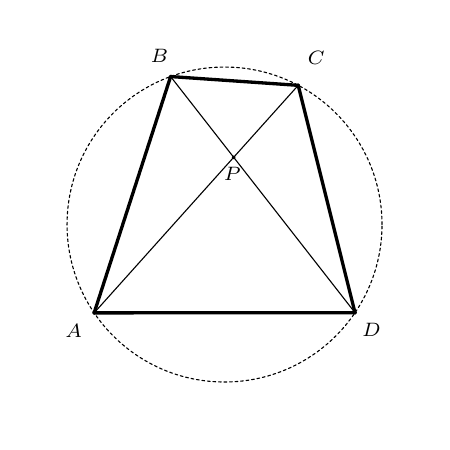
\begin{tikzpicture}[line cap=round,line join=round,>=triangle 45,x=1.0cm,y=1.0cm]
		\clip(-2.5,-2.5) rectangle (2.5,2.5);
		\draw [line width=0.4pt,dash pattern=on 1pt off 1pt] (0.,0.) circle (2.cm);
		\draw [line width=1.2pt] (-1.6556613537561036,-1.1219560961457031)--(-0.6845453549155284,1.8792013348929841);
		\draw [line width=1.2pt] (-0.6845453549155284,1.8792013348929841)--(0.9358381181972095,1.7675426491400725);
		\draw [line width=1.2pt] (0.9358381181972095,1.7675426491400725)--(1.6572015924511359,-1.1196798122576914);
		\draw [line width=1.2pt] (1.6572015924511359,-1.1196798122576914)--(-1.6556613537561036,-1.1219560961457031);
		\draw [line width=0.4pt] (-1.6556613537561036,-1.1219560961457031)--(0.9358381181972095,1.7675426491400725);
		\draw [line width=0.4pt] (-0.6845453549155284,1.8792013348929841)--(1.6572015924511359,-1.1196798122576914);
		\begin{scriptsize}
			\draw [fill=black] (-1.6556613537561036,-1.1219560961457031) circle (0.5pt);
			\draw[color=black] (-1.9141209085926902,-1.3450872021542477) node {$A$};
			\draw [fill=black] (-0.6845453549155284,1.8792013348929841) circle (0.5pt);
			\draw[color=black] (-0.8248807713547837,2.137180509318455) node {$B$};
			\draw [fill=black] (0.9358381181972095,1.7675426491400725) circle (0.5pt);
			\draw[color=black] (1.163807661026546,2.1124250516539567) node {$C$};
			\draw [fill=black] (1.6572015924511359,-1.1196798122576914) circle (0.5pt);
			\draw[color=black] (1.865212294853986,-1.3368353829327484) node {$D$};
			\draw [fill=black] (0.11624160914632323,0.8536998680886387) circle (0.5pt);
			\draw[color=black] (0.09932298145313719,0.6436012302270824) node {$P$};
		\end{scriptsize}
	\end{tikzpicture}
	\caption{}\label{fig:cocircle_angle}
\end{figure}

\switchcolumn*
\subsection{有关边的性质定理}
这一小节中的性质也大多是上一个小节中的结论外加相似三角形而推出的. 如图\ref{fig:cocircle_segment}中, 有如下定理:
\begin{theorem}
	\textbf{1. 相交弦定理}\quad{\kaishu 两条弦相交于圆内, 其交点分别将两条弦分为两部分, 则一条弦上的两部分的乘积等于另一条弦上的两部分的乘积. 即,}
	\[PA\cdot PC=PB\cdot PD.\]
\end{theorem}
\par
这个定理的证明并不困难, 只需要注意到
\[\angle PAD=\angle PBC,\ \angle PDA=\angle PCB,\]
所以有$\triangle PAB\sim\triangle PDC$, 于是
\[\frac{PA}{PB}=\frac{PD}{PC},\]
即得结论.
\begin{theorem}
	\textbf{2. 割线定理}\quad{\kaishu 两条割线相交于圆外, 两条割线被圆分别截得两条弦, 则两条割线的交点与其中一条弦的两端的距离之积等于此交点与另一条弦的两端的距离之积. 即,}
	\[QA\cdot QB=QC\cdot QD.\]
\end{theorem}
\par
与相交弦定理类似, 只需注意到$\triangle QAD\sim\triangle QCB$即可证明. 其中, 割线就是一条与圆有两个交点的直线.\par 

\switchcolumn
\begin{figure}[htbp]
	\centering
	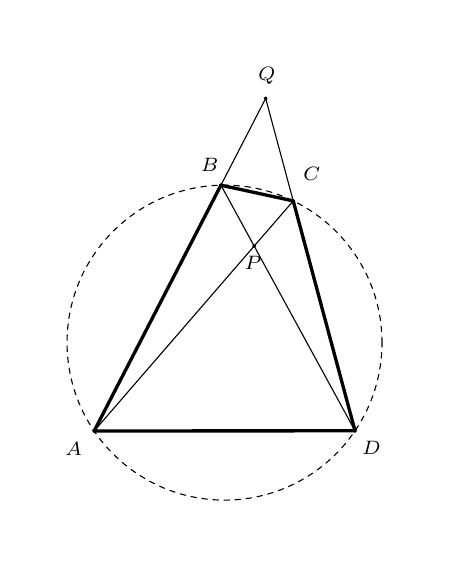
\begin{tikzpicture}[line cap=round,line join=round,>=triangle 45,x=1.0cm,y=1.0cm]
		\clip(-2.5,-2.5) rectangle (2.5,4.);
		\draw [line width=0.4pt,dash pattern=on 2pt off 2pt] (0.,0.) circle (2.cm);
		\draw [line width=1.2pt] (-1.6556613537561036,-1.1219560961457031)--(-0.04559898372086738,1.999480115600959);
		\draw [line width=1.2pt] (-0.04559898372086738,1.999480115600959)--(0.8726058565509365,1.7995996830164775);
		\draw [line width=1.2pt] (0.8726058565509365,1.7995996830164775)--(1.6572015924511359,-1.1196798122576914);
		\draw [line width=1.2pt] (1.6572015924511359,-1.1196798122576914)--(-1.6556613537561036,-1.1219560961457031);
		\draw [line width=0.4pt] (-1.6556613537561036,-1.1219560961457031)--(0.8726058565509365,1.7995996830164775);
		\draw [line width=0.4pt] (-0.04559898372086738,1.999480115600959)--(1.6572015924511359,-1.1196798122576914);
		\draw [line width=0.4pt] (-0.04559898372086738,1.999480115600959)--(0.5227468854887712,3.1013351803266644);
		\draw [line width=0.4pt] (0.5227468854887712,3.1013351803266644)--(0.8726058565509365,1.7995996830164775);
		\begin{scriptsize}
			\draw [fill=black] (-1.6556613537561036,-1.1219560961457031) circle (0.5pt);
			\draw[color=black] (-1.9141209085926902,-1.3450872021542477) node {$A$};
			\draw [fill=black] (-0.04559898372086738,1.999480115600959) circle (0.5pt);
			\draw[color=black] (-0.1894906912993381,2.2609577976409443) node {$B$};
			\draw [fill=black] (0.8726058565509365,1.7995996830164775) circle (0.5pt);
			\draw[color=black] (1.106044926476051,2.145432328539954) node {$C$};
			\draw [fill=black] (1.6572015924511359,-1.1196798122576914) circle (0.5pt);
			\draw[color=black] (1.865212294853986,-1.3368353829327484) node {$D$};
			\draw [fill=black] (0.37648840874398515,1.2263079079720325) circle (0.5pt);
			\draw[color=black] (0.36338119654111456,1.0149330951945505) node {$P$};
			\draw [fill=black] (0.5227468854887712,3.1013351803266644) circle (0.5pt);
			\draw[color=black] (0.5366694001925998,3.383205211764848) node {$Q$};
		\end{scriptsize}
	\end{tikzpicture}
	\caption{}\label{fig:cocircle_segment}
\end{figure}

\switchcolumn*
\begin{theorem}
	\textbf{3. 托勒密(Ptolemy)定理}\quad {\kaishu 圆内接四边形中, 两组对边乘积之和等于对角线乘积, 即}
	\[AB\cdot CD+AD\cdot BC=AC\cdot BD.\]
\end{theorem}
\par
如图\ref{fig:ptolemy}, 在对角线AC上找一点$E$, 使得$\angle BAD=\angle CED$. 由于$\angle CAD<\angle BAD=\angle CED<\angle BAD+\angle BDA=180^\circ -\angle ACD$,
所以这样的点$E$是存在的.\footnote{可能有同学对这里的叙述感到奇怪. 事实上, 我们考虑点$E$从点$A$至点$C$运动的过程, 此时$\angle DEC$是连续变化的, 范围为$\angle DAC\le\angle DEC\le 180^\circ-\angle DCA$. 则$E$运动的过程中, $\angle DEC$可以取遍这个范围内的所有值. 而$\angle BAD$在这个范围内, 所以存在这样的点$E$, 使得$\angle DEC=\angle DAB$.} 于是,结合$\angle CBD=\angle EAD$, $\angle ECD=\angle ABD$, 可得
\[\triangle AED\sim\triangle BCD,\ \triangle ABD\sim\triangle ECD.\]
所以, 有
\[AD\cdot BC=AE\cdot BD,\ AB\cdot CD=CE\cdot DB.\]
两式相乘, 得到
\[AD\cdot BC+AB\cdot CD=(AE+EC)\cdot BD=AC\cdot BD.\]

\switchcolumn
\begin{figure}[htbp]
	\centering
	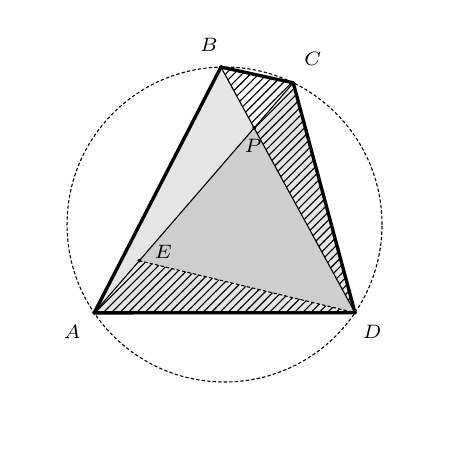
\begin{tikzpicture}[line cap=round,line join=round,>=triangle 45,x=1.0cm,y=1.0cm]
		\clip(-2.5,-2.5) rectangle (2.5,2.5);
		\fill[line width=0.4pt,fill=black,pattern=north east lines,pattern color=black](-0.04559898372086738,1.999480115600959) --(0.8726058565509365,1.7995996830164775) --(1.6572015924511359,-1.1196798122576914) -- cycle;
		\fill[line width=0.4pt,fill=black,pattern=north east lines,pattern color=black](-1.6556613537561036,-1.1219560961457031) --(-1.0824097170143592,-0.45953140250201563) --(1.6572015924511359,-1.1196798122576914) -- cycle;
		\fill[line width=0.pt,fill=black,fill opacity=0.10000000149011612](-0.04559898372086738,1.999480115600959) --(-1.6556613537561036,-1.1219560961457031) --(1.6572015924511359,-1.1196798122576914) -- cycle;
		\fill[line width=2.pt,fill=black,fill opacity=0.10000000149011612](0.8726058565509365,1.7995996830164775) --(-1.0824097170143592,-0.45953140250201563) --(1.6572015924511359,-1.1196798122576914) -- cycle;
		\draw [line width=0.4pt,dash pattern=on 1pt off 1pt] (0.,0.) circle (2.cm);
		\draw [line width=1.2pt] (-1.6556613537561036,-1.1219560961457031)--(-0.04559898372086738,1.999480115600959);
		\draw [line width=1.2pt] (-0.04559898372086738,1.999480115600959)--(0.8726058565509365,1.7995996830164775);
		\draw [line width=1.2pt] (0.8726058565509365,1.7995996830164775)--(1.6572015924511359,-1.1196798122576914);
		\draw [line width=1.2pt] (1.6572015924511359,-1.1196798122576914)--(-1.6556613537561036,-1.1219560961457031);
		\draw [line width=0.4pt] (-1.6556613537561036,-1.1219560961457031)--(0.8726058565509365,1.7995996830164775);
		\draw [line width=0.4pt] (-0.04559898372086738,1.999480115600959)--(1.6572015924511359,-1.1196798122576914);
		\draw [line width=0.4pt,dash pattern=on 1pt off 1pt](-1.0824097170143592,-0.45953140250201563)-- (1.6572015924511359,-1.1196798122576914);
		\begin{scriptsize}
			\draw [fill=black] (-1.6556613537561036,-1.1219560961457031) circle (0.5pt);
			\draw[color=black] (-1.9350129264455753,-1.367135049260033) node {$A$};
			\draw [fill=black] (-0.04559898372086738,1.999480115600959) circle (0.5pt);
			\draw[color=black] (-0.1985482828517931,2.283893175732024) node {$B$};
			\draw [fill=black] (0.8726058565509365,1.7995996830164775) circle (0.5pt);
			\draw[color=black] (1.1193838569014367,2.108128866159105) node {$C$};
			\draw [fill=black] (1.6572015924511359,-1.1196798122576914) circle (0.5pt);
			\draw[color=black] (1.8763043425705213,-1.3582301023698085) node {$D$};
			\draw [fill=black] (0.37648840874398515,1.2263079079720325) circle (0.5pt);
			\draw[color=black] (0.362463371232352,1.001580823539692) node {$P$};
			\draw [fill=black] (-1.0824097170143592,-0.45953140250201563) circle (0.5pt);
			\draw[color=black] (-0.7773698307163872,-0.34306615688421216) node {$E$};
		\end{scriptsize}
	\end{tikzpicture}
	\caption{}\label{fig:ptolemy}
\end{figure}
\end{paracol}

\section{四点共圆的判定}
\begin{paracol}{2}
事实上, 四点共圆的性质定理的逆命题就是判定定理(除了1.2.1节的第3个性质定理). 这也体现了有关四点共圆的定理均是等价命题(即条件和结论等价), 使用起来非常方便. 对于四点共圆的判定定理, 我们还是分两个方面叙述.\par

\subsection{有关角的判定定理}
\begin{theorem}
	\textbf{1. }{\kaishu 若一个四边形的对角互补, 那么这个四边形内接于圆.}\\
	\textbf{2. }{\kaishu 若一个四边形中, 存在一条边所对的两个边与对角线的夹角相等, 那么这个四边形内接于圆.}
\end{theorem}
\par
证明它们的基本思想, 就是利用同一法.\par
\subsection{有关边的判定定理}
\begin{theorem}
	\textbf{1. }{\kaishu 一个凸四边形的对角线交于其内部, 其交点分别将两个对角线分为两部分, 若两个对角线上的两个部分的乘积相等, 则此四边形内接于圆.}
\end{theorem}
\par
如图\ref{fig:cocircle_segment}, 只需要注意到$PA\cdot PC=PB\cdot PD$等价于
\[\frac{PB}{PA}=\frac{PC}{PD},\]
于是有$\triangle PBA\sim\triangle PCD$即可.
\begin{theorem}
	\textbf{2. }{\kaishu 一个四边形的一组对边相交于一点, 若其中一条对边的两个顶点到这个交点的距离之积等于另外一条对边上的两个顶点到这个交点的距离之积,那么这个四边形内接于圆.}
\end{theorem}
\par
同样地, 如图\ref{fig:cocircle_segment}, 只需注意到$\triangle QAB\sim\triangle QCD$即可.
\begin{theorem}
	\textbf{3. }{\kaishu 若一个四边形两组对边乘积之和等于两条对角线的乘积, 那么此四边形内接于圆. }
\end{theorem}
\par
类似于图\ref{fig:ptolemy}, 构造$\triangle EAD$相似于$\triangle CBD$, 通过$AE+EC=AC$证明$A$, $E$,
$C$共线即可.

\end{paracol}

\section{圆的切线}

\begin{paracol}{2}
切线, 就是某条直线与圆有且只有一个交点, 此时这条直线与圆心的距离等于圆的半径. 事实上, 我们可以把切线视为割线的极限情况. 如图\ref{fig:tangent}所示,当点$B$逐渐靠近$A$, 割线$AB$的极限情况就是点$A$处的切线. 对于切线, 首先有一个熟知的性质: \textbf{切线垂直于过切点的半径. }还有一个在直观上比较好理解的定理, 叫做\textbf{切线长定理}: 圆外一点向一圆引两条切线, 则两个切点到此点的距离相等. 我们还有两个比较常用的定理: \textbf{弦切角定理}与\textbf{切割线定理}.下面将一一介绍.
\begin{theorem}
	\textbf{弦切角定理}\quad {\kaishu 如图\ref{fig:xian_qie_jiao}, $A$处有一条切线$AD$, $AC$为一条弦, 则$\angle DAC$等于\\$\angle DAC$所夹的弧所对的圆周角, 即$\angle ABC$.}
\end{theorem}
\par
这个定理可以按照如下方式直观理解: 设想在弧$\wideparen{AC}$上有一个点$A'$, 连接$AA'$ 并延长至$D'$. 则由四点共圆的性质有
\[\angle ABC=\angle D'A'C.\]
在$A'$趋近于$A$的过程中, $\angle D'A'C$趋近于$\angle DAC$. 而$\angle D'A'C$恒等于$\angle ABC$, 那么极限情况也是如此, 即
\[\angle ABC=\angle DAC.\]\par
注意, 以上过程只是直观的理解, 不能作为严格的证明.
\begin{theorem}
	\textbf{切割线定理}\quad {\kaishu 如图\ref{fig:qie_ge_xian}, 过一点作一个圆的一条切线和割线,则割线与圆的两个交点与此点的距离的乘积等于这个点到切点的距离的平方. 即,}
	\[PA^2=PB\cdot PC.\]
\end{theorem}
\par
我们还是从直观理解一下这个定理: 设有一条割线$PA_1A_2$, 如图\ref{fig:qie_ge_xian}所示. 则由四点共圆的性质有
\[PA_1\cdot PA_2=PB\cdot PC\]
当$A_1$和$A_2$趋近于$A$时, $PA_1$和$PA_2$都趋近于$PA$, 所以$PA_1\cdot PA_2$趋近于$PA^2$. 又 $PA_1\cdot PA_2$在趋近的过程时恒等于$PB\cdot PC$, 所以在极限情况两者也是相等的, 即
\[PA^2=PB\cdot PC.\]\par
同样, 以上过程不能作为严格的证明过程.\par
以上就是切线最基本的性质, 相关结构与结论将在后面补充.
\switchcolumn
\begin{figure}[htbp]
	\vspace{1em}
	\centering
	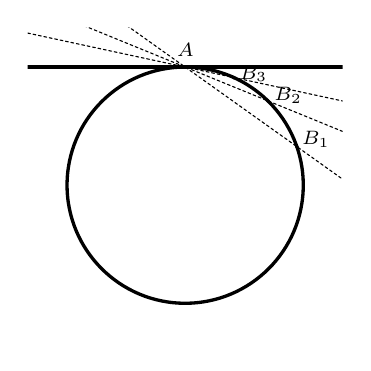
\begin{tikzpicture}[line cap=round,line join=round,>=triangle 45,x=1.cm,y=1.cm]
		\clip(-2.,-2.) rectangle (2.,2.);
		\draw [line width=1.2pt] (0.,0.) circle (1.5);
		\draw [line width=1.2pt,domain=-2.:2.] plot(\x,{(-1.5-0.*\x)/-1.});
		\draw [line width=0.4pt,dash pattern=on 1pt off 1pt,domain=-2.:2.]plot(\x,{(--0.9272280820482917-0.13329299508944636*\x)/0.6181520546988611});
		\draw [line width=0.4pt,dash pattern=on 1pt off 1pt,domain=-2.:2.]plot(\x,{(--1.5761634480320732-0.4295465581586162*\x)/1.0507756320213821});
		\draw [line width=0.4pt,dash pattern=on 1pt off 1pt,domain=-2.:2.]plot(\x,{(--2.1264292240451645-1.0097398626458354*\x)/1.4176194826967763});
		\begin{scriptsize}
			\draw [fill=black] (0.,1.5) circle (0.5pt);
			\draw[color=black] (0.0032040065994748193,1.718394680334216) node {$A$};
			\draw [fill=black] (0.6181520546988611,1.3667070049105536) circle (0.5pt);
			\draw[color=black] (0.8682082650947508,1.4119825135318147) node {$B_3$};
			\draw [fill=black] (1.0507756320213821,1.0704534418413838) circle (0.5pt);
			\draw[color=black] (1.30748942458138,1.1353980797809742) node {$B_2$};
			\draw [fill=black] (1.4176194826967763,0.4902601373541646) circle (0.5pt);
			\draw[color=black] (1.659998997008922,0.5822292122792931) node {$B_1$};
		\end{scriptsize}
	\end{tikzpicture}
	\caption{}\label{fig:tangent}
\end{figure}

\begin{figure}[htbp]
	\centering
	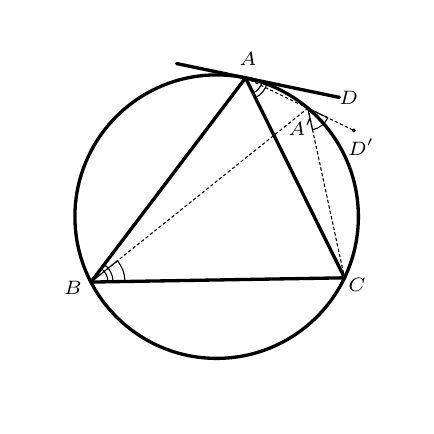
\begin{tikzpicture}[line cap=round,line join=round,>=triangle 45,x=1.2cm,y=1.2cm]
		\clip(-2.,-2.) rectangle (2.,2.);
		\draw [shift={(0.3057250661520829,1.4685135967795138)},line width=0.4pt] (0,0) --(-63.66591463534447:0.2346362429451152) arc(-63.66591463534447:-11.760239192061768:0.2346362429451152) -- cycle;
		\draw [shift={(-1.3306337946410773,-0.6923970714547305)},line width=0.4pt] (0,0) --(0.9593423412332046:0.2346362429451152) arc(0.9593423412332046:52.86501778451591:0.2346362429451152) -- cycle;
		\draw [shift={(-1.3306337946410773,-0.6923970714547305)},line width=0.4pt] (0,0) --(0.9593423412332046:0.36097883530017727) arc(0.9593423412332046:38.72085333369297:0.36097883530017727) -- cycle;
		\draw [shift={(0.9651551009623368,1.1482489412520185)},line width=0.4pt] (0,0) --(-77.81007908616742:0.2346362429451152) arc(-77.81007908616742:-25.904403642884702:0.2346362429451152) -- cycle;
		\draw [shift={(0.3057250661520829,1.4685135967795138)},line width=0.4pt] (0,0) --(-63.66591463534447:0.18048941765008863) arc(-63.66591463534447:-11.760239192061768:0.18048941765008863) -- cycle;
		\draw [shift={(-1.3306337946410773,-0.6923970714547305)},line width=0.4pt] (0,0) --(0.9593423412332046:0.18048941765008863) arc(0.9593423412332046:52.86501778451591:0.18048941765008863) -- cycle;
		\draw [line width=1.2pt] (0.,0.) circle (1.5);
		\draw [line width=1.2pt] (0.3057250661520829,1.4685135967795138)--(-1.3306337946410773,-0.6923970714547305);
		\draw [line width=1.2pt] (-1.3306337946410773,-0.6923970714547305)--(1.3530699957168189,-0.6474577875745167);
		\draw [line width=1.2pt] (1.3530699957168189,-0.6474577875745167)--(0.3057250661520829,1.4685135967795138);
		\draw [line width=0.4pt,dash pattern=on 1pt off 1pt](0.9651551009623368,1.1482489412520185)-- (1.3530699957168189,-0.6474577875745167);
		\draw [line width=0.4pt,dash pattern=on 1pt off 1pt](0.9651551009623368,1.1482489412520185)-- (-1.3306337946410773,-0.6923970714547305);
		\draw [line width=1.2pt] (-0.42342569956106385,1.6203131215311823)--(1.2962043497180982,1.2623089384402468);
		\draw [line width=0.4pt,dash pattern=on 1pt off 1pt](0.3057250661520829,1.4685135967795138)-- (1.4519463742314258,0.9118295620646947);
		\begin{scriptsize}
			\draw [fill=black] (0.3057250661520829,1.4685135967795138) circle (0.5pt);
			\draw[color=black] (0.330253810351815,1.6689744347344655) node {$A$};
			\draw [fill=black] (-1.3306337946410773,-0.6923970714547305) circle (0.5pt);
			\draw[color=black] (-1.5215676147380943,-0.7531935501297224) node {$B$};
			\draw [fill=black] (1.3530699957168189,-0.6474577875745167) circle (0.5pt);
			\draw[color=black] (1.485386083312382,-0.7170956665997047) node {$C$};
			\draw [fill=black] (0.9651551009623368,1.1482489412520185) circle (0.5pt);
			\draw[color=black] (0.8897710050670897,0.9470167641341113) node {$A'$};
			\draw [fill=black] (1.2962043497180982,1.2623089384402468) circle (0.5pt);
			\draw[color=black] (1.3987511628403395,1.2538487741392619) node {$D$};
			\draw [fill=black] (1.4519463742314258,0.9118295620646947) circle (0.5pt);
			\draw[color=black] (1.5287035435484035,0.7340392513070069) node {$D'$};
		\end{scriptsize}
	\end{tikzpicture}
	\caption{}\label{fig:xian_qie_jiao}
\end{figure}

\begin{figure}[htbp]
	\centering
	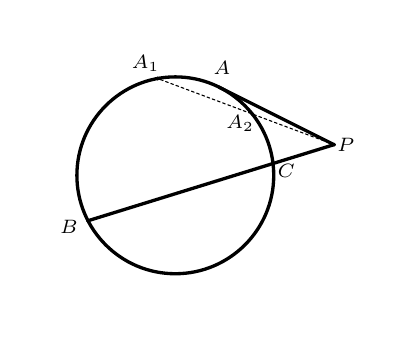
\begin{tikzpicture}[line cap=round,line join=round,>=triangle 45,x=1.25cm,y=1.25cm]
		\clip(-2.,-1.5) rectangle (1.5,1.5);
		\draw [line width=1.2pt] (-0.5,0.) circle (1);
		\draw [line width=1.2pt] (-1.387089196427385,-0.46159804763648704)--(0.49279482419897014,0.11982669587256368);
		\draw [line width=1.2pt] (0.49279482419897014,0.11982669587256368)--(1.1128585753599993,0.311604701069895);
		\draw [line width=1.2pt] (1.1128585753599993,0.311604701069895)--(-0.05278640450004196,0.8944271909999159);
		\draw [line width=0.4pt,dash pattern=on 1pt off 1pt](1.1128585753599993,0.311604701069895)-- (-0.6802489734850847,0.9836210182573232);
		\begin{scriptsize}
			\draw [fill=black] (-0.05278640450004196,0.8944271909999159) circle (0.5pt);
			\draw[color=black] (-0.027115236595360505,1.0950180866071841) node {$A$};
			\draw [fill=black] (-1.387089196427385,-0.46159804763648704) circle (0.5pt);
			\draw[color=black] (-1.5793242283861226,-0.5221670955376091) node {$B$};
			\draw [fill=black] (0.49279482419897014,0.11982669587256368) circle (0.5pt);
			\draw[color=black] (0.6262564552979604,0.04817946423667057) node {$C$};
			\draw [fill=black] (1.1128585753599993,0.311604701069895) circle (0.5pt);
			\draw[color=black] (1.232700898602258,0.308084225652798) node {$P$};
			\draw [fill=black] (-0.6802489734850847,0.9836210182573232) circle (0.5pt);
			\draw[color=black] (-0.8014148383142407,1.1365306526667043) node {$A_1$};
			\draw [fill=black] (0.28232553477672256,0.6228697758250235) circle (0.5pt);
			\draw[color=black] (0.15878886358423078,0.5264764210094052) node {$A_2$};
		\end{scriptsize}
	\end{tikzpicture}
	\caption{}\label{fig:qie_ge_xian}
\end{figure}

\end{paracol}

\section{圆幂与圆幂定理}
\begin{paracol}{2}
本节我们要重点讨论一个很重要的概念: 点到圆的\textbf{幂}. 对于点到圆的幂有很多种说法, 但它们实际上是统一的, 我们将在后面一一介绍这些说法. 首先我们从单方面给出“点到圆的幂”的定义: 
\begin{theorem}
	\textbf{点到圆的幂}\quad {\kaishu 平面上有一点$P$与半径为$r$的圆$\odot O$, 则$P$到$\odot O$的幂被定义为
	\[OP^2-r^2.\]}
\end{theorem}
\par
所以, 我们有
\[P\text{到}\odot O\text{的幂}\begin{cases}
>0,\ P\text{在}\odot O\text{外}; \\
=0,\ P\text{在}\odot O\text{上};\\
<0,\ P\text{在}\odot O\text{内};
\end{cases}\]\par
应当注意的是, 也有些地方将$P$到$\odot O$的幂定义为$\left|OP^2-r^2\right|$, 即对于$P$ 在$\odot O$ 内部的情况, 点$P$的幂也是正的. 这不是错误的, 只要在同一道题目内没有产生歧义. 但为了避免某些麻烦, 我们还是倾向于使用$OP^2-r^2$这种定义.\par
由于$P$在$\odot O$上的情况太过无聊, 我们就分$P$在$\odot O$的外部和内部分类讨论. 当然, 两者也可以统一. 

\subsection{点在圆外部的情况}
首先, 我们给出幂常用的第二个定义: \par
\switchcolumn[0]*
\begin{theorem}
	\textbf{点到圆的幂}\quad {\kaishu 对于点在圆的外部的情况, 点到圆的幂为, 从该点到过点所作的圆切线的切点的线段长度的平方. }
\end{theorem}
\par
事实上, 这里关于“切线长”的叙述可能会比较繁琐, 但相对严谨. 一般我们会说“切线长的平方”, 这样也不会引起歧义, 但我们要记住, 切线是一条直线, 所以实际上我们是把“从该点到过点所作的圆切线的切点的线段长度”简称为“切线长”.\par
我们下面证明两者等价. \par
事实上这很容易: 如图\ref{fig:tangent_length}, 设切点为$A$, 连接$AO$, $PO$. 由于$AP$为切线, 所以由切线的性质有$AP\perp OA$. 所以$\triangle OAP$为直角三角形, $\angle OAP=90^\circ$. 于是, 我们可以利用勾股定理, 即得
\[AP^2=OP^2-r^2.\]

\switchcolumn
\begin{figure}[htbp]
	\centering
	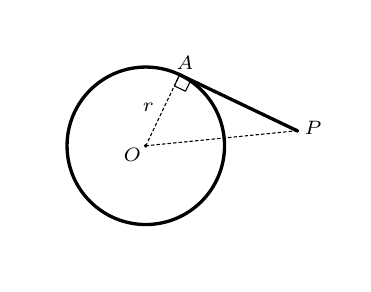
\begin{tikzpicture}[line cap=round,line join=round,>=triangle 45,x=1.0cm,y=1.0cm]
		\clip(-1.5,-1.5) rectangle (2.5,1.5);
		\draw[line width=0.4pt] (0.36267970162037344,0.7605797186299835) -- (0.5047305536653386,0.6928432810513062) -- (0.5724669912440158,0.8348941330962714) -- (0.4304161391990507,0.9026305706749486) -- cycle; 
		\draw [line width=1.2pt] (0.,0.) circle (1.cm);
		\draw [line width=0.4pt,dash pattern=on 1pt off 1pt] (0.,0.)-- (0.4304161391990507,0.9026305706749486);
		\draw [line width=0.4pt,dash pattern=on 1pt off 1pt] (0.,0.)-- (1.9223126899463303,0.1912250695551909);
		\draw [line width=1.2pt] (1.9223126899463303,0.1912250695551909)-- (0.4304161391990507,0.9026305706749486);
			\begin{scriptsize}
			\draw [fill=black] (1.9223126899463303,0.1912250695551909) circle (0.5pt);
			\draw[color=black] (2.12690131991075,0.2213243461977229) node {$P$};
			\draw [fill=black] (0.,0.) circle (0.5pt);
			\draw[color=black] (-0.17154544193126534,-0.11858679463806746) node {$O$};
			\draw [fill=black] (0.4304161391990507,0.9026305706749486) circle (0.5pt);
			\draw[color=black] (0.4961371561390384,1.0589625146859207) node {$A$};
			\draw[color=black] (0.030782618090038835,0.49244394662627) node {$r$};
		\end{scriptsize}
	\end{tikzpicture}
	\caption{}\label{fig:tangent_length}
\end{figure}

\switchcolumn
还有一种常见的定义形式:
\begin{theorem}
	\textbf{点到圆的幂}\quad {\kaishu 对于点在圆的外部的情况, 点到圆的幂为, 该点到过该点所作的圆的割线与圆的两个交点所成的两条线段的长度的乘积的相反数. }
\end{theorem}
\par
我们仍然可以证明这与给出的第一个定义是等价的: 如图\ref{fig:mi_ge_xian}, 设割线为$PAB$. 作$OM$垂直于$AB$于$M$, 则由垂径定理有$MA=MB$. 则
\begin{align*}
PO^2-r^2&=OP^2-OB^2=(PM^2+OM^2)-(BM^2+OM^2)\\
&=PM^2-BM^2=(PM-BM)(PM+BM)\\
&=(PM-BM)(PM+AM)=PA\cdot PB.
\end{align*}
即, $PA\cdot PB=PO^2-r^2$. 


\switchcolumn
\begin{figure}[htbp]
	\centering
	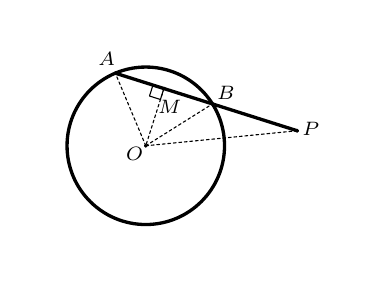
\begin{tikzpicture}[line cap=round,line join=round,>=triangle 45,x=1.0cm,y=1.0cm]
		\clip(-1.5,-1.5) rectangle (2.5,1.5);
		\draw[line width=0.4pt] (0.0912025445713372,0.7708555378651836) -- (0.04723699721317892,0.6319640126332269) -- (0.18612852244513564,0.5879984652750687) -- (0.23009406980329386,0.7268899905070254) -- cycle; 
		\draw [line width=1.2pt] (0.,0.) circle (1.cm);
		\draw [line width=0.4pt,dash pattern=on 1pt off 1pt] (0.,0.)-- (1.9223126899463303,0.1912250695551909);
		\draw [line width=1.2pt] (1.9223126899463303,0.1912250695551909)-- (-0.386797731909513,0.9221645810752311);
		\draw [line width=0.4pt,dash pattern=on 1pt off 1pt] (0.23009406980329386,0.7268899905070254)-- (0.,0.);
		\draw [line width=0.4pt,dash pattern=on 1pt off 1pt] (0.,0.)-- (0.8469858715161007,0.5316153999388198);
		\draw [line width=0.4pt,dash pattern=on 1pt off 1pt] (0.,0.)-- (-0.386797731909513,0.9221645810752311);
		\begin{scriptsize}
			\draw [fill=black] (1.9223126899463303,0.1912250695551909) circle (0.5pt);
			\draw[color=black] (2.0963109538930103,0.21638418475829027) node {$P$};
			\draw [fill=black] (0.,0.) circle (0.5pt);
			\draw[color=black] (-0.14252963897753113,-0.10295964213888793) node {$O$};
			\draw [fill=black] (-0.386797731909513,0.9221645810752311) circle (0.5pt);
			\draw[color=black] (-0.49621151177763195,1.0988719644633957) node {$A$};
			\draw [fill=black] (0.8469858715161007,0.5316153999388198) circle (0.5pt);
			\draw[color=black] (1.0180963125412466,0.6765139998574503) node {$B$};
			\draw [fill=black] (0.23009406980329386,0.7268899905070254) circle (0.5pt);
			\draw[color=black] (0.30386495776046024,0.49108855198166945) node {$M$};
		\end{scriptsize}
	\end{tikzpicture}
	\caption{}\label{fig:mi_ge_xian}
\end{figure}

\switchcolumn
\subsection{点在圆内部的情况}
\switchcolumn[0]*
在圆内部的点没有“切线”一说, 于是我们是这么定义的: 
\begin{theorem}
	\textbf{点到圆的幂}\quad {\kaishu 对于点在圆内部的情况, 点到圆的幂为, 该点到过这个点的一条弦的两个端点到这个点的距离之积的相反数.}
\end{theorem}
\par
如图\ref{fig:mi_xian}(图中未画出圆), 与图\ref{fig:mi_ge_xian}类似, 此处就略去证明过程.

\switchcolumn
\begin{figure}[htbp]
	\centering
	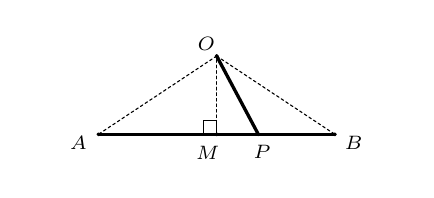
\begin{tikzpicture}[line cap=round,line join=round,>=triangle 45,x=1.2cm,y=1.2cm]
		\clip(-2.,-1.2) rectangle (2.,0.3);
		\draw[line width=0.4pt] (0.,-0.686083616528325) -- (-0.14214713800313986,-0.686083616528325) -- (-0.14214713800313986,-0.8282307545314647) -- (0.,-0.8282307545314647) -- cycle; 
		\draw [line width=0.4pt,dash pattern=on 1pt off 1pt] (0.,0.)-- (-1.2506133764070497,-0.8282307545314647);
		\draw [line width=0.4pt,dash pattern=on 1pt off 1pt] (0.,0.)-- (1.2506133764070495,-0.8282307545314647);
		\draw [line width=1.2pt] (1.2506133764070495,-0.8282307545314647)-- (-1.2506133764070497,-0.8282307545314647);
		\draw [line width=1.2pt] (0.4407283775484121,-0.8282307545314647)-- (0.,0.);
		\draw [line width=0.4pt,dash pattern=on 1pt off 1pt] (0.,-0.8282307545314647)-- (0.,0.);
		\begin{scriptsize}
			\draw [fill=black] (0.,0.) circle (0.5pt);
			\draw[color=black] (-0.1087438109235194,0.12999216937761346) node {$O$};
			\draw [fill=black] (-1.2506133764070497,-0.8282307545314647) circle (0.5pt);
			\draw[color=black] (-1.462321641061692,-0.9186956049621039) node {$A$};
			\draw [fill=black] (1.2506133764070495,-0.8282307545314647) circle (0.5pt);
			\draw[color=black] (1.4492108698048225,-0.9220460451357132) node {$B$};
			\draw [fill=black] (0.4407283775484121,-0.8282307545314647) circle (0.5pt);
			\draw[color=black] (0.480933659631724,-1.015858369996774) node {$P$};
			\draw [fill=black] (0.,-0.8282307545314647) circle (0.5pt);
			\draw[color=black] (-0.09534205022908204,-1.0225592503439926) node {$M$};
		\end{scriptsize}
	\end{tikzpicture}
	\caption{}\label{fig:mi_xian}
\end{figure}

\switchcolumn
\subsection{两者的统一表述}
这里我们只是提一下, 不必理解.
\begin{theorem}
	\textbf{点到圆的幂*}\quad {\kaishu 过$P$作直线$PAB$交$\odot O$于$A$, $B$, 则$P$到$\odot O$的幂被定义为$\overrightarrow{PA}\cdot\overrightarrow{PB}$.}
\end{theorem}
\par
有了前面的讨论, 我们会发现, 相交弦定理、切割线定理、割线定理的本质是一样的, 都和点到圆的幂有关, 所以我们统称为\textbf{圆幂定理}. 看完以上讨论, 我们的脑海中应该有这样的一个动画: \par
如图\ref{fig:motion_graph}, 设想平面内有一点$P$和$\odot O$, 有一条过$P$的转动的直线, 交$\odot O$于$A$, $B$两点. 则在直线$PAB$转动的过程中, $PA\cdot PB$为定值. 但我们要强调的是, 如果存在一条过$P$的线段$AB$, 满足在$AB$转动时$PA\cdot PB$为定值, 那么$A$和$B$的轨迹也不一定为一个圆. 另外, 以上只是对于这条直线与$\odot O$有交点时才有意义. 不过, 当直线与$\odot O$没有交点时, 在解析几何中有一种概念叫做“虚交点”, 此时如果用距离公式算出两个“虚交点”与$P$的距离(此时这个“距离”为虚数)的乘积, 那么结果是实数并且恒等于$P$到$\odot O$的幂.

\end{paracol}
\setcounter{figure}{12}
\begin{figure}[htbp]
	\centering
	\begin{minipage}{0.4\textwidth}
		\centering
		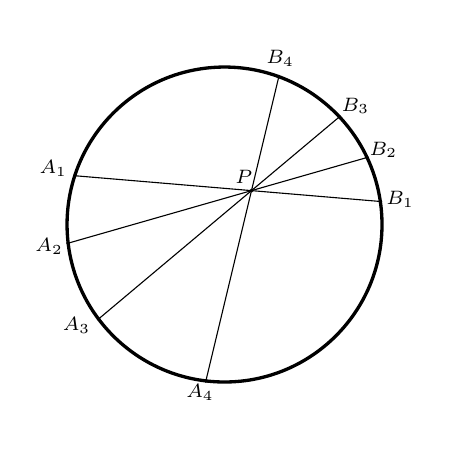
\begin{tikzpicture}[line cap=round,line join=round,>=triangle 45,x=1.0cm,y=1.0cm]
			\clip(-2.5,-2.5) rectangle (2.5,2.5);
			\draw [line width=1.2pt] (0.,0.) circle (2.cm);
			\draw [line width=0.4pt] (-1.9015756067219713,0.6196855750458988)-- (1.9784642520525804,0.2927101012094093);
			\draw [line width=0.4pt] (0.6894312551004229,1.8774143241412258)-- (-0.2369078267071474,-1.9859191024925704);
			\draw [line width=0.4pt] (-1.6,-1.2)-- (1.4591002370249182,1.3678547065802813);
			\draw [line width=0.4pt] (-1.985907734950381,-0.23700309758365465)-- (1.8097964254205239,0.8512560710709176);
			\begin{scriptsize}
				\draw [fill=black] (0.3425119341187099,0.43057370668774975) circle (0.5pt);
				\draw[color=black] (0.2469549176946053,0.6064854869230346) node {$P$};
				\draw [fill=black] (-1.9015756067219713,0.6196855750458988) circle (0.5pt);
				\draw[color=black] (-2.174546748507173,0.7129012552135158) node {$A_1$};
				\draw [fill=black] (-1.985907734950381,-0.23700309758365465) circle (0.5pt);
				\draw[color=black] (-2.2266687574657764,-0.2730734142533917) node {$A_2$};
				\draw [fill=black] (-1.6,-1.2) circle (0.5pt);
				\draw[color=black] (-1.8791886977417542,-1.2764220867065001) node {$A_3$};
				\draw [fill=black] (-0.2369078267071474,-1.9859191024925704) circle (0.5pt);
				\draw[color=black] (-0.31118492823710503,-2.13643523452345) node {$A_4$};
				\draw [fill=black] (1.9784642520525804,0.2927101012094093) circle (0.5pt);
				\draw[color=black] (2.2298624913241495,0.3176426872774427) node {$B_1$};
				\draw [fill=black] (0.6894312551004229,1.8774143241412258) circle (0.5pt);
				\draw[color=black] (0.7051942464556593,2.1115084956026977) node {$B_4$};
				\draw [fill=black] (1.4591002370249182,1.3678547065802813) circle (0.5pt);
				\draw[color=black] (1.6607644106967197,1.5077618918322122) node {$B_3$};
				\draw [fill=black] (1.8097964254205239,0.8512560710709176) circle (0.5pt);
				\draw[color=black] (2.0169314719138423,0.9474502955272295) node {$B_2$};
			\end{scriptsize}
		\end{tikzpicture}
		\centerline{(A)}
	\end{minipage}
	\quad
	\begin{minipage}{0.4\textwidth}
		\centering
		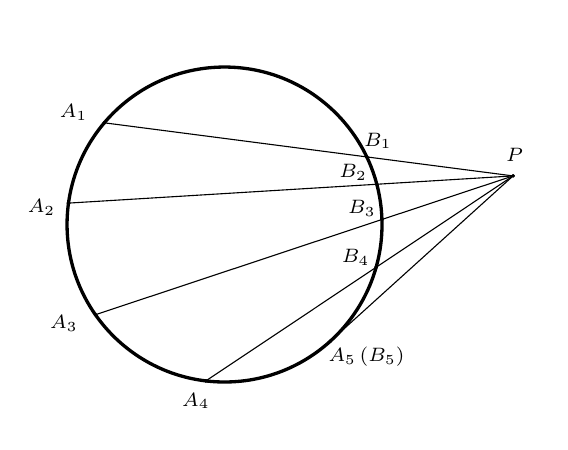
\begin{tikzpicture}[line cap=round,line join=round,>=triangle 45,x=1.0cm,y=1.0cm]
			\clip(-2.5,-2.5) rectangle (4.,2.5);
			\draw [line width=1.2pt] (0.,0.) circle (2.cm);
			\draw [line width=0.4pt] (-1.5269366989453965,1.2916904882415663)-- (1.8062787358143777,0.8586950148596487);
			\draw [line width=0.4pt] (1.9246831936108413,-0.5436861265766981)-- (-0.2369078267071474,-1.9859191024925704);
			\draw [line width=0.4pt] (-1.6394752368055279,-1.145478479894519)-- (1.9989852665200027,0.06370168157869094);
			\draw [line width=0.4pt] (-1.9814216079749924,0.27197134306723375)-- (1.93351203834367,0.5114012099908509);
			\draw [line width=0.4pt] (1.8062787358143777,0.8586950148596487)-- (3.6647142220545463,0.6172782301169876);
			\draw [line width=0.4pt] (3.6647142220545463,0.6172782301169876)-- (1.93351203834367,0.5114012099908509);
			\draw [line width=0.4pt] (3.6647142220545463,0.6172782301169876)-- (1.9989852665200027,0.06370168157869094);
			\draw [line width=0.4pt] (3.6647142220545463,0.6172782301169876)-- (1.9246831936108413,-0.5436861265766981);
			\draw [line width=0.4pt] (1.3413664538001928,-1.4834877945637082)-- (3.6647142220545463,0.6172782301169876);
			\begin{scriptsize}
				\draw [fill=black] (3.6647142220545463,0.6172782301169876) circle (0.5pt);
				\draw[color=black] (3.6832640935210788,0.8800680758928636) node {$P$};
				\draw [fill=black] (-1.5269366989453965,1.2916904882415663) circle (0.5pt);
				\draw[color=black] (-1.915705444127323,1.4211059936667259) node {$A_1$};
				\draw [fill=black] (-1.9814216079749924,0.27197134306723375) circle (0.5pt);
				\draw[color=black] (-2.3238026163910384,0.2215476388309625) node {$A_2$};
				\draw [fill=black] (-1.6394752368055279,-1.145478479894519) circle (0.5pt);
				\draw[color=black] (-2.039371253904206,-1.2562587880027873) node {$A_3$};
				\draw [fill=black] (-0.2369078267071474,-1.9859191024925704) circle (0.5pt);
				\draw[color=black] (-0.36369953142743455,-2.239401975729006) node {$A_4$};
				\draw [fill=black] (1.8062787358143777,0.8586950148596487) circle (0.5pt);
				\draw[color=black] (1.9488511114002873,1.0624751453137657) node {$B_1$};
				\draw [fill=black] (1.9246831936108413,-0.5436861265766981) circle (0.5pt);
				\draw[color=black] (1.6644197489134551,-0.41533128151998405) node {$B_4$};
				\draw [fill=black] (1.9989852665200027,0.06370168157869094) circle (0.5pt);
				\draw[color=black] (1.7448025252684296,0.20918105785327423) node {$B_3$};
				\draw [fill=black] (1.93351203834367,0.5114012099908509) circle (0.5pt);
				\draw[color=black] (1.6335032964692344,0.6605612635388965) node {$B_2$};
				\draw [fill=black] (1.3413664538001928,-1.4834877945637082) circle (0.5pt);
				\draw[color=black] (1.8036541962035066,-1.6767225412441888) node {$A_5\,(B_5)$};
			\end{scriptsize}
		\end{tikzpicture}
		\centerline{(B)}
	\end{minipage}
	\caption{}\label{fig:motion_graph}
\end{figure}

\begin{paracol}{2}
\begin{tcolorbox}
\textbf{例}\quad{\kaishu 如图\ref{fig:example1}, $\triangle ABC$内有一点$P$, 满足$\angle ABP=\angle ACP$. 过$P$作$PE$, $PF$平行于$AB$, $AC$, 交$AC$, $AB$于$E$, $F$. 设$O$为$\triangle ABC$的外接圆的圆心, 求证: $OE=OF$.}
\end{tcolorbox}

\textbf{分析}\quad 首先, 我们可以看看通过条件能得到什么. 条件$\angle ABP=\angle ACP$比较特别, 我们可能需要利用它来导出或构造相似三角形. 另外, $AE\parallel PF$, $AF\parallel PE$这两个条件表明四边形$AEPF$为一个平行四边形, 于是我们有$AE=PF$, $AF=PE$, 并且我们还发现了$\angle BFP=\angle CEP=\angle A$. 结合$\angle FBP=\angle ECP$, 我们可以得到一组相似三角形. 至于如何证明$OE=OF$, 就需要用到圆幂的知识.\par

\textbf{证明}\quad 如图\ref{fig:solution1}, 由题意, 因为$AF\parallel PE$, $AE\parallel PF$, 所以$AFPE$为平行四边形, 于是有
\[AF=PE,\ AE=PF.\]
并且, 还有
\[\angle BFP=\angle CEP=\angle A\]
结合$\angle FBP=\angle ECP$, 有$\triangle FBP\sim\triangle ECP$. 于是, $BF/FP=CE/EP$.
结合$AF=PE, AE=PF$, 有
\[AF\cdot FB=AE\cdot EC.\]\par
现在我们考虑$E$和$F$到$\triangle ABC$的外接圆的幂. 由圆幂的定义, 我们可以得到
\[OF^2-R^2=-AF\cdot FB,\ OE^2-R^2=-AE\cdot EC.\]
式中, $R$为三角形外接圆的半径. 结合$AF\cdot FB=AR\cdot EC$, 即得$OE=OF$.

\switchcolumn
\begin{figure}[H]
	\centering
	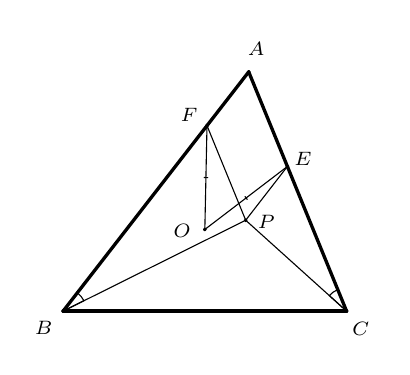
\begin{tikzpicture}[line cap=round,line join=round,>=triangle 45,x=0.9cm,y=0.9cm]
		\clip(-0.5,-0.5) rectangle (4.5,4.);
		\draw [shift={(0.,0.)},line width=0.4pt] (0,0) -- (26.468306316028198:0.3281050635671744) arc (26.468306316028198:52.19981175940985:0.3281050635671744) -- cycle;
		\draw [shift={(4.,0.)},line width=0.4pt] (0,0) -- (112.24407555044822:0.3281050635671744) arc (112.24407555044822:137.97558099382988:0.3281050635671744) -- cycle;
		\draw [line width=1.2pt] (0.,0.)-- (4.,0.);
		\draw [line width=1.2pt] (4.,0.)-- (2.619063817235214,3.37645382191942);
		\draw [line width=1.2pt] (2.619063817235214,3.37645382191942)-- (0.,0.);
		\draw [line width=0.4pt] (2.5765054427828287,1.2828192140218995)-- (0.,0.);
		\draw [line width=0.4pt] (2.5765054427828287,1.2828192140218995)-- (4.,0.);
		\draw [line width=0.4pt] (2.5765054427828287,1.2828192140218995)-- (3.1650314754621176,2.0415372564240712);
		\draw [line width=0.4pt] (2.5765054427828287,1.2828192140218995)-- (2.0305377845559245,2.6177357795172482);
		\draw [line width=0.4pt] (2.0305377845559245,2.6177357795172482)-- (2.,1.1526413260613302);
		\draw [line width=0.4pt] (2.0415115973582023,1.8846415613840493) -- (1.989026187197722,1.8857355441945294);
		\draw [line width=0.4pt] (2.,1.1526413260613302)-- (3.1650314754621176,2.0415372564240712);
		\draw [line width=0.4pt] (2.5665938743368515,1.617957281936155) -- (2.598437601125266,1.5762213005492465);
		\begin{scriptsize}
			\draw [fill=black] (0.,0.) circle (0.5pt);
			\draw[color=black] (-0.27482284342726393,-0.22942082668382288) node {$B$};
			\draw [fill=black] (4.,0.) circle (0.5pt);
			\draw[color=black] (4.200530223628994,-0.25566923176919676) node {$C$};
			\draw [fill=black] (2.619063817235214,3.37645382191942) circle (0.5pt);
			\draw[color=black] (2.7240574375767097,3.701277834850922) node {$A$};
			\draw [fill=black] (2.,1.1526413260613302) circle (0.5pt);
			\draw[color=black] (1.6806833354330954,1.1354962377556213) node {$O$};
			\draw [fill=black] (2.5765054427828287,1.2828192140218995) circle (0.5pt);
			\draw[color=black] (2.8684236655462665,1.2536140606398039) node {$P$};
			\draw [fill=black] (2.0305377845559245,2.6177357795172482) circle (0.5pt);
			\draw[color=black] (1.7791148545032476,2.776021555591491) node {$F$};
			\draw [fill=black] (3.1650314754621176,2.0415372564240712) circle (0.5pt);
			\draw[color=black] (3.386829665982402,2.1526219348138604) node {$E$};
		\end{scriptsize}
	\end{tikzpicture}
	\caption{}\label{fig:example1}
\end{figure}
\begin{figure}[htbp]
	\centering
	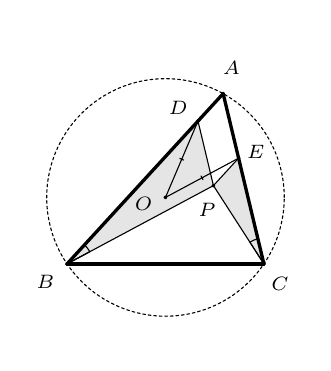
\begin{tikzpicture}[line cap=round,line join=round,>=triangle 45,x=1.0cm,y=1.0cm]
		\clip(-0.5,-1.) rectangle (3.,3.);
		\draw [shift={(0.,0.)},line width=0.4pt] (0,0) -- (28.136212227118488:0.3281050635671744) arc (28.136212227118488:47.48551708735234:0.3281050635671744) -- cycle;
		\draw [shift={(2.5,0.)},line width=0.4pt] (0,0) -- (103.45735625064013:0.3281050635671744) arc (103.45735625064013:122.80666111087397:0.3281050635671744) -- cycle;
		\fill[line width=2.pt,fill=black,fill opacity=0.10000000149011612] (1.8591243597394502,0.9941904769355673) -- (1.6629750989752177,1.8138981320214773) -- (0.,0.) -- cycle;
		\fill[line width=2.pt,fill=black,fill opacity=0.10000000149011612] (1.8591243597394502,0.9941904769355673) -- (2.1786892546791283,1.3427574316349653) -- (2.5,0.) -- cycle;
		\draw [line width=1.2pt] (0.,0.)-- (2.5,0.);
		\draw [line width=1.2pt] (2.5,0.)-- (1.9825399939148958,2.1624650867208755);
		\draw [line width=1.2pt] (1.9825399939148958,2.1624650867208755)-- (0.,0.);
		\draw [line width=0.4pt] (1.8591243597394502,0.9941904769355673)-- (0.,0.);
		\draw [line width=0.4pt] (1.8591243597394502,0.9941904769355673)-- (2.5,0.);
		\draw [line width=0.4pt] (1.8591243597394502,0.9941904769355673)-- (2.1786892546791283,1.3427574316349653);
		\draw [line width=0.4pt] (1.8591243597394502,0.9941904769355673)-- (1.6629750989752177,1.8138981320214773);
		\draw [line width=0.4pt] (1.6629750989752177,1.8138981320214773)-- (1.25,0.8440298334496851);
		\draw [line width=0.4pt] (1.4806377613702573,1.3186806935949875) -- (1.43233733760496,1.3392472718761754);
		\draw [line width=0.4pt] (1.25,0.8440298334496851)-- (2.1786892546791283,1.3427574316349653);
		\draw [line width=0.4pt] (1.7019260575341217,1.116518465374439) -- (1.7267631971450064,1.0702687997102105);
		\draw [line width=0.4pt,dash pattern=on 1pt off 1pt] (1.25,0.8440298334496851) circle (1.5082726410543628cm);
		\begin{scriptsize}
			\draw [fill=black] (0.,0.) circle (0.5pt);
			\draw[color=black] (-0.27482284342726315,-0.22942082668382438) node {$B$};
			\draw [fill=black] (2.5,0.) circle (0.5pt);
			\draw[color=black] (2.70437113376268,-0.2556692317691983) node {$C$};
			\draw [fill=black] (1.9825399939148958,2.1624650867208755) circle (0.5pt);
			\draw[color=black] (2.0875336142563925,2.4872890996523767) node {$A$};
			\draw [fill=black] (1.25,0.8440298334496851) circle (0.5pt);
			\draw[color=black] (0.9719763981279994,0.7614564652890413) node {$O$};
			\draw [fill=black] (1.8591243597394502,0.9941904769355673) circle (0.5pt);
			\draw[color=black] (1.7791148545032485,0.6892733513042629) node {$P$};
			\draw [fill=black] (1.6629750989752177,1.8138981320214773) circle (0.5pt);
			\draw[color=black] (1.411637183308013,1.9754452004875855) node {$D$};
			\draw [fill=black] (2.1786892546791283,1.3427574316349653) circle (0.5pt);
			\draw[color=black] (2.395952374009536,1.4176665924233895) node {$E$};
		\end{scriptsize}
	\end{tikzpicture}
	\caption{}\label{fig:solution1}
\end{figure}



\end{paracol}



\chapter{三角形的五心}
\thispagestyle{empty}
\setcounter{figure}{-1}

三角形的五个“心”就是外心、垂心、内心、重心、旁心.\footnote{事实上, 三角形有三个旁心, 所以有时候会戏称为三角形的“七心”.} 
本章将重点介绍外心、内心与垂心,并且介绍各个心之间的联系. 本章的某些内容很丰富, 但也可能比较难, 可以拓宽同学们的视野, 欣赏一下整个平面几何体系中的冰山一角. 对于中考来说, 本章的某些较难的结构与结论也许不会经常考到, 我们也不要求同学们完全掌握, 但本章内容可以提高同学们思考几何问题的高度, 站在更高的角度往往很利于解题. 应当指出的是, 三角形绝非只有这几个“心”,\footnote{事实上, 截止2023年1月19日, 三角形的“心”的数量已经达到了惊人的52802. 相关资料可以查询:https://faculty.evansville.edu/ck6/en\-cyclo\-pedia/ETC.html (不含连字符)}平面几何的内容也不只有三角形(但三角形仍然占大多数), 如果想了解更多的内容, 可以参考相关的数学竞赛书籍.

\section{外心与外接圆}\label{sec:circumcenter}


\begin{paracol}{2}
外心与外接圆是一个三角形很重要的几何结构. 前面提到了, 每个三角形都存在一个外接圆(这一点将会稍后证明), 而这个圆的圆心就称为外心.\par
\switchcolumn[0]*
首先我们要说明外心的存在性, 即此三角形所在的平面上存在一个点, 到三个顶点的距离相等. 如图\ref{fig:circumcenter}所示, 这是不难证明的: 考虑任意两条边的中垂线的交点(容易知道这两个中垂线不平行, 故交点存在), 则由中垂线的性质, 这个点到三个顶点的距离都相等. 于是, 这个点满足要求, 我们便证明了存在性. 顺便指出, 这个点也在第三条边的中垂线上. 以这个点为圆心, 过任意一个顶点画圆, 这个圆就是三角形的外接圆.
\par
将上面这段话总结一下就是: \textbf{三角形三条边的中垂线交于一点, 这个点被称为外心; 三角形所在平面上存在唯一一个圆同时过三角形的三个顶点, 这个圆的圆心即为外心.}\par
所以, 我们可以看到, 外心最基本的性质就是到三个顶点的距离相等.\par
作为三角形最重要的一个心之一, 外心单独的性质反而不是很多. 相反地, 它更多的是和其他几何结构融为一体, 作为外接圆的圆心使用. 不过, 外心的一些关于角度的结论是必须熟知的:\par
\begin{theorem}
\textbf{1. }$\angle AOB=2\angle ACB$, $\angle BOC=2\angle BAC$, $\angle COA=2\angle CBA$;\\
\textbf{2. }$\angle OAB=\angle OBA=90^\circ-\angle ACB$, $\angle OBC=\angle OCB=90^\circ-\angle BAC$, $\angle OCA=\angle OAC=90^\circ-\angle CBA$.
\end{theorem}\par
\switchcolumn[0]

这些结论都不难证明: 第一条即为“同弧所对的圆心角是圆周角的2倍”, 第二条注意到$\triangle AOB$, $\triangle BOC$, $\triangle COA$均为等腰三角形即可. 应当注意的是, 这两条定理虽然简单, 但将其熟记会在一些题中起到很大的作用. \par
必须要强调的是, 以上的有关角度的性质都是在$\triangle ABC$为锐角三角形的假设下推出的. 即, 以上有关角度的定理对于直角三角形和钝角三角形可能不成立. 至于哪些成立, 哪些不成立, 不成立的要怎么修改, 三种情况(锐角三角形, 直角三角形, 钝角三角形)下的定理有哪些相通之处, 留给大家探索. \par
我们将给出一个例题, 来介绍外心的性质是如何运用的:

\switchcolumn
\stepcounter{figure}
\begin{figure}[htbp]
	\centering
	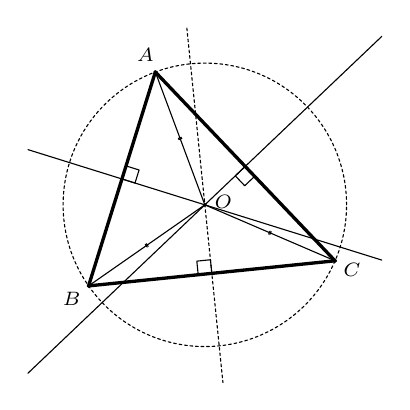
\begin{tikzpicture}[line cap=round,line join=round,>=triangle 45,x=0.9cm,y=0.9cm]
		\clip(-2.5,-2.5) rectangle (2.5,2.5);
		\draw[line width=0.4pt] (-0.9852618740186195,0.3075916848773176) --(-0.9277446389143748,0.49182793583377715) -- (-1.1119808898708343,0.5493451709380219) --(-1.169498124975079,0.36510891998156236) -- cycle;
		\draw[line width=0.4pt] (0.42971263398073484,0.40904399693268023) --(0.5627848952222337,0.2692477101844164) -- (0.7025811819704976,0.4023199714259152) --
		(0.5695089207289987,0.5421162581741791) -- cycle;
		\draw[line width=0.4pt] (0.07886986583271119,-0.7748563069603908) --(-0.11314379367042778,-0.7944006939996701) -- (-0.0935994066311485,-0.986414353502809) --(0.09841425287199045,-0.9668699664635297) -- cycle;
		\draw [line width=0.4pt,dash pattern=on 1pt off 1pt] (0.,0.) circle (2.);
		\draw [line width=1.2pt] (-0.6984034571180708,1.8740951446192713)--(-1.6405927928320876,-1.1438773046561466);
		\draw [line width=1.2pt] (-1.6405927928320876,-1.1438773046561466)--(1.8374212985760685,-0.7898626282709129);
		\draw [line width=1.2pt] (1.8374212985760685,-0.7898626282709129)--(-0.6984034571180708,1.8740951446192713);
		\draw [line width=0.4pt,dash pattern=on 1pt off 1pt,domain=-2.5:2.5]plot(\x,{(-0.--3.478014091408156*\x)/-0.35401467638523365});
		\draw [line width=0.4pt,domain=-2.5:2.5]plot(\x,{(-0.-2.535824755694139*\x)/-2.663957772890184});
		\draw [line width=0.4pt,domain=-2.5:2.5]plot(\x,{(-0.--0.9421893357140168*\x)/-3.017972449275418});
		\draw [line width=0.4pt] (0.,0.)-- (-0.6984034571180708,1.8740951446192713);
		\draw [line width=0.4pt] (-0.3679272834148256,0.9207728271446176) --(-0.3243922315043865,0.9369966730082389);
		\draw [line width=0.4pt] (-0.3740112256136843,0.9370984716110327) --(-0.3304761737032452,0.953322317474654);
		\draw [line width=0.4pt] (0.,0.)-- (-1.6405927928320876,-1.1438773046561466);
		\draw [line width=0.4pt] (-0.7998645382184507,-0.5860117793948251) --(-0.8264366991785577,-0.5479009649012812);
		\draw [line width=0.4pt] (-0.8141560936535294,-0.5959763397548652) --(-0.8407282546136363,-0.5578655252613213);
		\draw [line width=0.4pt] (0.,0.)-- (1.8374212985760685,-0.7898626282709129);
		\draw [line width=0.4pt] (0.9198817807753876,-0.37014942183719063) --(0.9015333470671967,-0.41283254379315015);
		\draw [line width=0.4pt] (0.9358879515088724,-0.3770300844777617) --(0.9175395178006814,-0.41971320643372123);
		\begin{scriptsize}
			\draw [fill=black] (-0.6984034571180708,1.8740951446192713) circle (0.5pt);
			\draw[color=black] (-0.8385544793470171,2.1136066961617024) node {$A$};
			\draw [fill=black] (-1.6405927928320876,-1.1438773046561466) circle (0.5pt);
			\draw[color=black] (-1.8780927218880201,-1.3302266995188172) node {$B$};
			\draw [fill=black] (1.8374212985760685,-0.7898626282709129) circle (0.5pt);
			\draw[color=black] (2.076798580740042,-0.9178958882316051) node {$C$};
			\draw[color=black] (-0.3681489059066748,4.088148609368072) node {$i$};
			\draw [fill=black] (0.,0.) circle (0.5pt);
			\draw[color=black] (0.26033142968679595,0.04614516351032809) node {$O$};
		\end{scriptsize}
	\end{tikzpicture}
	\caption{}\label{fig:circumcenter}
\end{figure}

\switchcolumn*
\begin{tcolorbox}
\textbf{例}\quad {\kaishu 如图\ref{fig:example2}, $\triangle ABC$的外心为$O$, $\angle BAC=60^\circ$. $AB$上有一点$D$, $AC$上有一点$E$, 使得$D$, $O$, $E$共线, 且$AD=AE$. 求证: $AB+AC=3DE$.}
\end{tcolorbox}\par
\textbf{分析}\quad 这道题中出现了一个外心, 我们要立刻想到上述所有性质.\par
首先我们要立刻注意到$\triangle ADE$为一个等边三角形, 并且$\triangle BOC$为一个顶角为$120^\circ$的等腰三角形. 于是$\angle BDO=\angle BOC=\angle OEC$, 这就是一线三等角模型. 于是我们便揭露了这个题的本质.\par


\switchcolumn
\begin{figure}[htbp]
	\centering
	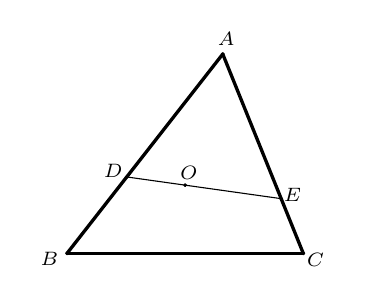
\begin{tikzpicture}[line cap=round,line join=round,>=triangle 45,x=1.0cm,y=1.0cm]
		\clip(-2.,-1.2) rectangle (2.,2.);
		\draw [line width=1.2pt] (0.4775653376155419,1.6649118139733867)-- (-1.5,-0.8660254037844386);
		\draw [line width=1.2pt] (-1.5,-0.8660254037844386)-- (1.5,-0.8660254037844386);
		\draw [line width=1.2pt] (1.5,-0.8660254037844386)-- (0.4775653376155419,1.6649118139733867);
		\draw [line width=0.4pt] (-0.7418359731794906,0.10429174131623863)-- (1.2194013107950328,-0.1714307349117291);
		\begin{scriptsize}
			\draw [fill=black] (0.,0.) circle (0.5pt);
			\draw[color=black] (0.04575970924203199,0.1558408888957056) node {$O$};
			\draw [fill=black] (0.4775653376155419,1.6649118139733867) circle (0.5pt);
			\draw[color=black] (0.5205004073536457,1.859322217413171) node {$A$};
			\draw [fill=black] (-1.5,-0.8660254037844386) circle (0.5pt);
			\draw[color=black] (-1.7228821072522154,-0.9332701244187394) node {$B$};
			\draw [fill=black] (1.5,-0.8660254037844386) circle (0.5pt);
			\draw[color=black] (1.6561546263657412,-0.9472330861278988) node {$C$};
			\draw [fill=black] (1.2194013107950328,-0.1714307349117291) circle (0.5pt);
			\draw[color=black] (1.3629324304732737,-0.11876402471776557) node {$E$};
			\draw [fill=black] (-0.7418359731794906,0.10429174131623863) circle (0.5pt);
			\draw[color=black] (-0.9130303281206388,0.17911249174430485) node {$D$};
		\end{scriptsize}
	\end{tikzpicture}
	\caption{}\label{fig:example2}
\end{figure}

\switchcolumn*
\textbf{证明}\quad 如图\ref{fig:solution2}, 连接$OB$, $OC$. \par
因为$O$为$\triangle ABC$的外心, 所以$BO=CO$, $\angle BOC=2\angle A=120^\circ$. 因为$AD=AE$, $\angle A=60^\circ$, 所以$\triangle ADE$为等边三角形, 所以$AD=DE=EA$. 所以, $\angle BDO=\angle BOC=\angle OEC=120^\circ.$
所以, 
\begin{align*}
	\angle DBO&=60^\circ-\angle DOB=\angle EOC,\\
	\angle DOB&=60^\circ-\angle EOC=\angle ECO.
\end{align*}
又因为$BO=CO$, 于是, 在$\triangle BDO$与$\triangle OEC$中,
\[\angle DBO=\angle EOC,\ BO=OC,\ \angle DOB=\angle ECO,\]
所以$\triangle BDO\cong\triangle OEC$(ASA). 于是我们有
\[BD=OE,\ DO=EC.\]
又因为$AD=AE=DE$, 所以
\begin{align*}
	AB+AC&=AD+AE+BD+EC\\
	&=DE+DE+OE+DO=3DE.
\end{align*}\par

\switchcolumn
\begin{figure}[htbp]
	\centering
	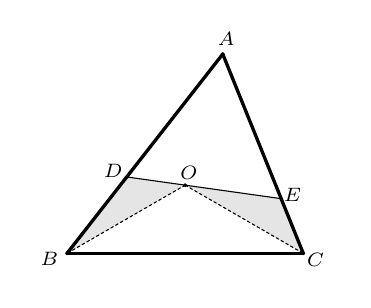
\begin{tikzpicture}[line cap=round,line join=round,>=triangle 45,x=1.0cm,y=1.0cm]
		\clip(-2.,-1.2) rectangle (2.,2.);
		\fill[line width=2.pt,fill=black,fill opacity=0.10000000149011612] (-1.5,-0.8660254037844386) -- (-0.7418359731794906,0.10429174131623863) -- (0.,0.) -- cycle;
		\fill[line width=2.pt,fill=black,fill opacity=0.10000000149011612] (0.,0.) -- (1.2194013107950328,-0.1714307349117291) -- (1.5,-0.8660254037844386) -- cycle;
		\draw [line width=1.2pt] (0.4775653376155419,1.6649118139733867)-- (-1.5,-0.8660254037844386);
		\draw [line width=1.2pt] (-1.5,-0.8660254037844386)-- (1.5,-0.8660254037844386);
		\draw [line width=1.2pt] (1.5,-0.8660254037844386)-- (0.4775653376155419,1.6649118139733867);
		\draw [line width=0.4pt] (-0.7418359731794906,0.10429174131623863)-- (1.2194013107950328,-0.1714307349117291);
		\draw [line width=0.4pt,dash pattern=on 1pt off 1pt] (0.,0.)-- (-1.5,-0.8660254037844386);
		\draw [line width=0.4pt,dash pattern=on 1pt off 1pt] (0.,0.)-- (1.5,-0.8660254037844386);
		\begin{scriptsize}
			\draw [fill=black] (0.,0.) circle (0.5pt);
			\draw[color=black] (0.04575970924203199,0.1558408888957056) node {$O$};
			\draw [fill=black] (0.4775653376155419,1.6649118139733867) circle (0.5pt);
			\draw[color=black] (0.5205004073536457,1.859322217413171) node {$A$};
			\draw [fill=black] (-1.5,-0.8660254037844386) circle (0.5pt);
			\draw[color=black] (-1.7228821072522154,-0.9332701244187394) node {$B$};
			\draw [fill=black] (1.5,-0.8660254037844386) circle (0.5pt);
			\draw[color=black] (1.6561546263657412,-0.9472330861278988) node {$C$};
			\draw [fill=black] (1.2194013107950328,-0.1714307349117291) circle (0.5pt);
			\draw[color=black] (1.3629324304732737,-0.11876402471776557) node {$E$};
			\draw [fill=black] (-0.7418359731794906,0.10429174131623863) circle (0.5pt);
			\draw[color=black] (-0.9130303281206388,0.17911249174430485) node {$D$};
		\end{scriptsize}
	\end{tikzpicture}
	\caption{}\label{fig:solution2}
\end{figure}

\switchcolumn*
\textbf{注1}\quad 这道题是笔者自己出的, 自我感觉不错, 因为这道题很好地隐藏了一线三等角的结构, 充分利用了外心的性质. \par
\textbf{注2}\quad 我们在此想要特别强调一点: 在平面几何中, 我们非常注重对于点的“刻画”.\par
\switchcolumn[0]*
事实上, 所谓刻画, 就是指约束这个点的条件. 一般来说, 平面上的一个定点至少有两个刻画条件, 一个完全自由的动点没有刻画条件, 一个“不太自由”(相对于“完全自由”)的动点(例如在一条直线上的动点)有一个刻画条件. 如果一个点有三个或以上的刻画方式, 那么这个点可能就是解题的重要线索, 沟通各个关系的桥梁. 当然, 这里的刻画条件一般是指基本的数量关系或其他(例如点在直线上), 而不是类似于“$O$为$\triangle ABC$的外心”的(对于$O$的)刻画. 如果我们想利用这个点的性质, 我们就需要好好理解对于这个点的刻画是什么. 即, 对于这个点的约束条件是什么. 如果做题做到一半发现无路可走, 那么有时候就是漏掉了某个点的某个刻画条件. 顺便指出, 如果在一个证明题中没有用到某个点的所有性质(即对这个点的刻画不充分), 但依然证了出来, 那很可能是证明的过程出了点问题(例如“循环论证”), 即“伪证”.\par
例如, 在这道题中, 我们对于$O$运用了它的两个刻画条件: $BO=OC$ 与 $\angle BOC=120^\circ$. 注意, 这两个条件可以刻画, 也恰好可以刻画点$O$(当然, 并不是所有的题对每个点需要的刻画是恰好足够的, 即, 一个刻画可能需要反复利用, 并不是说某一个刻画已经用过就不会再使用了). $BO=OC$说明了$O$在 $BC$ 的中垂线上, $\angle BOC=120^\circ$说明了$O$在某个圆弧上(因为此时$\angle BOC$为一个定值). 这两个条件缺一不可, 否则就无法充分刻画点$O$. 当然, 也可以从另外的角度刻画$O$, 例如$OA=OB$并且$OB=OC$. 对一个点的刻画也许有许多方式, 我们要选择足够的并且尽量简单的、有利于解题的条件来刻画一个点, 帮助我们解题.\par
以上的说明可能对于某些同学有些难以理解, 相信多做些难题就会有所体会.
\switchcolumn
{\kaishu 这里的文字解释可能比较多, 也比较抽象, 但请大家务必理解, 这对解题有很大的帮助.}

\end{paracol}

\section{内心与内切圆}

\begin{paracol}{2}
内心与内切圆是一个三角形又一个重要的结构. 每个三角形都存在一个唯一的与三条边(线段)相切的圆, 被称为内切圆, 这个圆的圆心就是内心.\par
我们知道, 直线与圆相切的充分必要条件是直线与圆心的距离等于圆的半径, 所以一个三角形的内心到三条边的距离都等于内切圆的半径, 且在三角形内部. \par

\switchcolumn*
\begin{figure}[htbp]
	\centering
	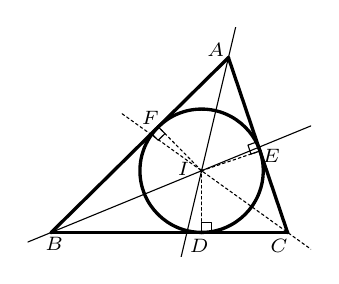
\begin{tikzpicture}[line cap=round,line join=round,>=triangle 45,x=1.0cm,y=1.0cm]
		\clip(-0.3,-0.3) rectangle (3.3,2.6);
		\draw[line width=0.4pt] (2.029241830851238,0.) -- (2.029241830851238,0.12062565976196463) -- (1.9086161710892733,0.12062565976196463) -- (1.9086161710892733,0.) -- cycle; 
		\draw[line width=0.4pt] (2.6117772488882682,1.1481507288469917) -- (2.497507154084786,1.1095127264838731) -- (2.5361451564479043,0.9952426316803906) -- (2.650415251251387,1.0338806340435092) -- cycle; 
		\draw[line width=0.4pt] (1.272784402400568,1.2557587083521742) -- (1.3575033769908555,1.1698911059786397) -- (1.4433709793643903,1.254610080568927) -- (1.3586520047741026,1.3404776829424618) -- cycle; 
		\draw [line width=1.2pt] (2.2495405157280497,2.2194490183008226)-- (0.,0.);
		\draw [line width=1.2pt] (0.,0.)-- (3.,0.);
		\draw [line width=1.2pt] (2.2495405157280497,2.2194490183008226)-- (3.,0.);
		\draw [line width=0.4pt,domain=-0.3:3.3] plot(\x,{(--1.676192933386476-0.972969852735326*\x)/-0.23093216681137763});
		\draw [line width=0.4pt,domain=-0.3:3.3] plot(\x,{(-0.--0.3795708909560573*\x)/0.9251626552876121});
		\draw [line width=0.4pt,dash pattern=on 1pt off 1pt,domain=0.9:3.3] plot(\x,{(-1.748882551544003--0.5829608505146676*\x)/-0.8125002441644036});
		\draw [line width=0.4pt,dash pattern=on 1pt off 1pt] (1.9086161710892733,0.)-- (1.9086161710892735,0.7830570510093465);
		\draw [line width=0.4pt,dash pattern=on 1pt off 1pt] (1.9086161710892735,0.7830570510093465)-- (2.650415251251387,1.0338806340435092);
		\draw [line width=0.4pt,dash pattern=on 1pt off 1pt] (1.9086161710892735,0.7830570510093465)-- (1.3586520047741026,1.3404776829424618);
		\draw [line width=1.2pt] (1.9086161710892735,0.7830570510093465) circle (0.7830570510093465cm);
		\begin{scriptsize}
			\draw [fill=black] (0.,0.) circle (0.5pt);
			\draw[color=black] (0.03647692921372073,-0.14833426016755447) node {$B$};
			\draw [fill=black] (3.,0.) circle (0.5pt);
			\draw[color=black] (2.8926483631355993,-0.172704323596922) node {$C$};
			\draw [fill=black] (2.2495405157280497,2.2194490183008226) circle (0.5pt);
			\draw[color=black] (2.08843626996647,2.3179161588844406) node {$A$};
			\draw [fill=black] (1.9086161710892735,0.7830570510093465) circle (0.5pt);
			\draw[color=black] (1.6790192043530945,0.8020982135777796) node {$I$};
			\draw [fill=black] (1.9086161710892733,0.) circle (0.5pt);
			\draw[color=black] (1.8788537244739085,-0.1678303109110485) node {$D$};
			\draw [fill=black] (2.650415251251387,1.0338806340435092) circle (0.5pt);
			\draw[color=black] (2.795168109418129,0.9678146448974788) node {$E$};
			\draw [fill=black] (1.3586520047741026,1.3404776829424618) circle (0.5pt);
			\draw[color=black] (1.2598541133679722,1.4600899261707032) node {$F$};
		\end{scriptsize}
	\end{tikzpicture}
	\caption{}\label{fig:incenter1}
\end{figure}

\switchcolumn
首先我们要说明内心的存在性, 即此三角形内部存在一点, 到三条边的距离相等. 如图\ref{fig:incenter1}所示, 这是不难证明的:考虑任意两个三角形的内角的内角平分线(所在直线)的交点(容易知道这两个角平分线不平行, 故交点存在), 则由角平分线的性质, 这个点到三个顶点的距离相等.于是, 这个点满足要求, 我们便证明了存在性. 顺便指出, 这个点也在第三个三角形的内角的内角平分线上. 以这个点为圆心, 做一个与任意一条边相切的圆, 这个圆就是三角形的内切圆.\par
将上面这段话总结一下就是: \textbf{三角形三个内角的角平分线交于一点, 这个点被称为内心; 三角形所在平面上存在唯一一个圆同时与三条边(线段)相切, 这个圆的圆心即为内心.}\par
内心与内切圆本身有一些有趣的性质, 下面为大家一一列出.\par
首先是关于角度的一些结论, 这是必须熟记的:
\begin{theorem}
	{\kaishu 如图\ref{fig:incenter1}, $\angle BIC=90^\circ+\angle BAC/2$, $\angle CIA=90^\circ+\angle CBA/2$, $\angle AIB=90^\circ+\angle ACB/2$.}
\end{theorem}\par
这些定理的证明都很容易, 例如:
\begin{align*}
	\angle BIC&=180^\circ-\angle IBC-\angle ICB=180^\circ-B/2-C/2\\
	&=90^\circ+\frac{180^\circ-B-C}{2}=90^\circ+A/2.
\end{align*}
其中, $A$, $B$, $C$分别为$\triangle ABC$的三个内角, 以后都采用这种记法. 顺便指出, 也一般用$a$, $b$, $c$表示$A$, $B$, $C$的对边.\par
还有一些关于边长与面积的定理:
\begin{theorem}
	{\kaishu 如图\ref{fig:incenter1}, 记周长$l=a+b+c$, 半周长$p=l/2$, 内切圆半径为$r$, 则有
	\begin{align*}
		AE&=AF=p-a=\frac{-a+b+c}{2},\\
		BF&=BD=p-b=\frac{a-b+c}{2},\\
		CD&=CE=p-c=\frac{a+b-c}{2}.
	\end{align*}
	另外, 还有$S_{\triangle ABC}=pr$.}
\end{theorem}\par
这些定理也不难证明, 利用三元一次方程组即可.\par
还有一个与角平分线定理有关的定理:\par

\switchcolumn*
\begin{figure}[htbp]
	\centering
	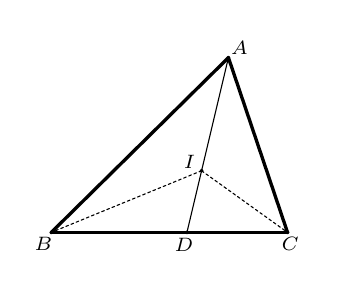
\begin{tikzpicture}[line cap=round,line join=round,>=triangle 45,x=1.0cm,y=1.0cm]
		\clip(-0.3,-0.3) rectangle (3.3,2.6);
		\draw [line width=1.2pt] (2.2495405157280497,2.2194490183008226)-- (0.,0.);
		\draw [line width=1.2pt] (0.,0.)-- (3.,0.);
		\draw [line width=1.2pt] (2.2495405157280497,2.2194490183008226)-- (3.,0.);
		\draw [line width=0.4pt,dash pattern=on 1pt off 1pt] (1.9086161710892735,0.7830570510093465)-- (0.,0.);
		\draw [line width=0.4pt,dash pattern=on 1pt off 1pt] (1.9086161710892735,0.7830570510093465)-- (3.,0.);
		\draw [line width=0.4pt] (2.2495405157280497,2.2194490183008226)-- (1.722759372938604,0.);
		\begin{scriptsize}
			\draw [fill=black] (0.,0.) circle (0.5pt);
			\draw[color=black] (-0.09835367918963826,-0.15157719527634655) node {$B$};
			\draw [fill=black] (3.,0.) circle (0.5pt);
			\draw[color=black] (3.0346189132956343,-0.14671987342753218) node {$C$};
			\draw [fill=black] (2.2495405157280497,2.2194490183008226) circle (0.5pt);
			\draw[color=black] (2.388595107403322,2.3402289131654275) node {$A$};
			\draw [fill=black] (1.9086161710892735,0.7830570510093465) circle (0.5pt);
			\draw[color=black] (1.7571432670574534,0.8976043240675583) node {$I$};
			\draw [fill=black] (1.722759372938604,0.) circle (0.5pt);
			\draw[color=black] (1.6842834393252377,-0.15643451712516093) node {$D$};
		\end{scriptsize}
	\end{tikzpicture}
	\caption{}\label{fig:incenter2}
\end{figure}

\switchcolumn
\begin{theorem}
	{\kaishu 如图\ref{fig:incenter2}, 
	\[\frac{AI}{ID}=\frac{AB+AC}{BC}.\]}
\end{theorem}\par
证明也不难: 因为$BI$, $CI$平分$\angle ABD$, $\angle ACD$, 所以
\[\frac{AB}{BD}=\frac{AI}{ID}=\frac{AC}{CD}.\]
由比例的性质, 有
\[\frac{AI}{ID}=\frac{AB+AC}{BD+CD}=\frac{AB+AC}{BC}.\]
这个定理能帮助我们在已知边长的情况下方便地计算出比例$AI/ID$.\par
以下的定理不太常用, 可以作为兴趣了解:
\begin{theorem}
	{\kaishu 如图\ref{fig:incenter1}, $AD$, $BE$, $CF$三线共点(图中未画出三条线段). }
\end{theorem}\par
这个定理的证明并不困难: 注意到$AE=AF$, $BD=BF$, $CD=CE$, 所以
\[\frac{AF}{FB}\cdot\frac{BD}{DC}\cdot\frac{CE}{EA}=1.\]
由塞瓦定理的逆定理, 知此三线共点.\par
另外还有著名的“鸡爪定理”:

\switchcolumn*
\begin{figure}[htbp]
	\centering
	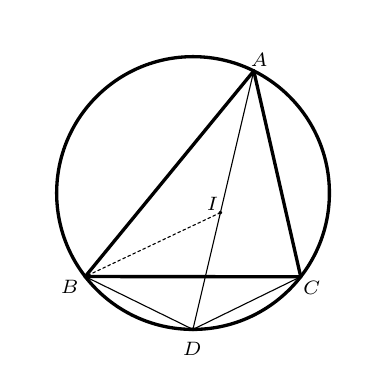
\begin{tikzpicture}[line cap=round,line join=round,>=triangle 45,x=1.0cm,y=1.0cm]
		\clip(-2.1,-2.1) rectangle (2.1,2.1);
		\draw [line width=1.2pt] (0.,0.) circle (1.7320508075688772cm);
		\draw [line width=1.2pt] (0.7715590901779906,1.5507084092000376)-- (-1.3691625576260107,-1.0608458374311511);
		\draw [line width=1.2pt] (-1.3691625576260107,-1.0608458374311511)-- (1.367571200284572,-1.062896519964298);
		\draw [line width=1.2pt] (1.367571200284572,-1.062896519964298)-- (0.7715590901779906,1.5507084092000376);
		\draw [line width=0.4pt] (-0.0012978556391126106,-1.732050321315966)-- (-1.3691625576260107,-1.0608458374311511);
		\draw [line width=0.4pt] (-0.0012978556391126106,-1.732050321315966)-- (1.367571200284572,-1.062896519964298);
		\draw [line width=0.4pt] (0.3478721289538606,-0.24892874032938647)-- (0.7715590901779906,1.5507084092000376);
		\draw [line width=0.4pt] (0.3478721289538606,-0.24892874032938647)-- (-0.0012978556391126106,-1.732050321315966);
		\draw [line width=0.4pt,dash pattern=on 1pt off 1pt] (0.3478721289538606,-0.24892874032938647)-- (-1.3691625576260107,-1.0608458374311511);
		\begin{scriptsize}
			\draw [fill=black] (0.7715590901779906,1.5507084092000376) circle (0.5pt);
			\draw[color=black] (0.8398671866323044,1.6923783489673068) node {$A$};
			\draw [fill=black] (-1.3691625576260107,-1.0608458374311511) circle (0.5pt);
			\draw[color=black] (-1.5666208062095253,-1.1897162235408927) node {$B$};
			\draw [fill=black] (1.367571200284572,-1.062896519964298) circle (0.5pt);
			\draw[color=black] (1.5065294008655141,-1.2019112640451586) node {$C$};
			\draw [fill=black] (0.3478721289538606,-0.24892874032938647) circle (0.5pt);
			\draw[color=black] (0.24637521542469104,-0.13687772667259404) node {$I$};
			\draw [fill=black] (-0.0012978556391126106,-1.732050321315966) circle (0.5pt);
			\draw[color=black] (-0.009720635164895606,-1.974263829315339) node {$D$};
		\end{scriptsize}
	\end{tikzpicture}
	\caption{}\label{fig:incenter2}
\end{figure}

\switchcolumn
\begin{theorem}
	\textbf{鸡爪定理}\quad {\kaishu 如图\ref{fig:incenter2}, $\triangle ABC$中$\angle BAC$的平分线交其外接圆于另一点$D$, 内心$I$在$AD$上, 则\[BD=ID=CD.\]}
\end{theorem}\par
这个定理的证明只需要计算角度: 显然$BD=CD$(因为$\angle BAD=\angle CAD$), 下面通过证明$\angle BID=\angle IBD$来证明$BD=ID$.\par
如图, 连接$BI$, 我们有

\begin{align*}
	\angle BID&=\angle ABI+\angle BAI=\frac{A+C}{2};\\
	\angle IBD&=\angle IBC+\angle CBD=\angle IBC+\angle CAI\\
	&=\frac{A+C}{2}.
\end{align*}
所以, $\angle BID=\angle IBD$, 即得$BD=ID$.\par
易知$D$是(不含$A$的)弧$\wideparen{BC}$的中点, 所以这条定理说明了$\triangle BIC$的外心就是弧 $BC$ 的中点.\par
下面我们举一道例题:

\switchcolumn*
\begin{figure}[htbp]
	\centering
	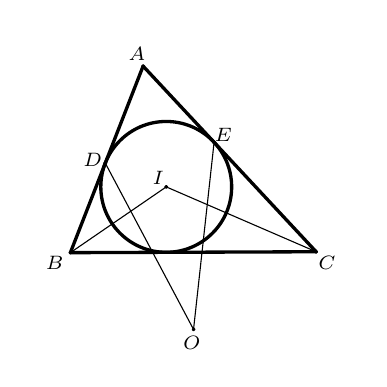
\begin{tikzpicture}[line cap=round,line join=round,>=triangle 45,x=1.0cm,y=1.0cm]
		\clip(-2.1,-2.1) rectangle (2.1,2.1);
		\draw [line width=1.2pt] (-0.6340158510493051,1.6118386707788794)-- (-1.5576981968828558,-0.7573482207200986);
		\draw [line width=1.2pt] (-1.5576981968828558,-0.7573482207200986)-- (1.5633062367195063,-0.7457034331648841);
		\draw [line width=1.2pt] (1.5633062367195063,-0.7457034331648841)-- (-0.6340158510493051,1.6118386707788794);
		\draw [line width=0.4pt] (-0.3402375351289607,0.07804942118450325)-- (-1.5576981968828558,-0.7573482207200986);
		\draw [line width=0.4pt] (-0.3402375351289607,0.07804942118450325)-- (1.5633062367195063,-0.7457034331648841);
		\draw [line width=0.4pt] (0.006462414177680453,-1.7320387516458733)-- (0.2675514321616571,0.6445326752039305);
		\draw [line width=0.4pt] (0.006462414177680453,-1.7320387516458733)-- (-1.1143353886865677,0.3798493863305266);
		\draw [line width=1.2pt] (-0.3402375351289607,0.07804942118450325) circle (0.830849388183343cm);
		\begin{scriptsize}
			\draw [fill=black] (-0.6340158510493051,1.6118386707788794) circle (0.5pt);
			\draw[color=black] (-0.7129679709109034,1.7696136054943248) node {$A$};
			\draw [fill=black] (-1.5576981968828558,-0.7573482207200986) circle (0.5pt);
			\draw[color=black] (-1.7576764407763599,-0.8848402109342424) node {$B$};
			\draw [fill=black] (1.5633062367195063,-0.7457034331648841) circle (0.5pt);
			\draw[color=black] (1.7016500489337707,-0.8848402109342424) node {$C$};
			\draw [fill=black] (-0.3402375351289607,0.07804942118450325) circle (0.5pt);
			\draw[color=black] (-0.44061206631562866,0.18832335344116613) node {$I$};
			\draw [fill=black] (0.006462414177680453,-1.7320387516458733) circle (0.5pt);
			\draw[color=black] (-0.013785648666317617,-1.909223613292587) node {$O$};
			\draw [fill=black] (0.2675514321616571,0.6445326752039305) circle (0.5pt);
			\draw[color=black] (0.3845856744730393,0.7411651896345585) node {$E$};
			\draw [fill=black] (-1.1143353886865677,0.3798493863305266) circle (0.5pt);
			\draw[color=black] (-1.2739398341071406,0.4200291230222203) node {$D$};
		\end{scriptsize}
	\end{tikzpicture}
	\caption{}\label{fig:example3}
\end{figure}

\switchcolumn
\begin{tcolorbox}
	\textbf{例}\quad {\kaishu 如图\ref{fig:example3}, $\triangle ABC$的内切圆$\odot I$与边$AB$, $AC$分别相切于$D$, $E$, $\triangle BCI$ 的外心为 $O$. 求证:
	\[\angle ODB=\angle OEC.\]}
\end{tcolorbox}\par
\textbf{分析}\quad 原题想要证明$\angle BDO=\angle CEO$, 我们可以立马想到这等价于$\angle ADO=\angle AEO$. 而且, $O$为$\triangle BIC$的外心, 由鸡爪定理的推论我们可以得到$O$为$\triangle ABC$外接圆上不含$A$的弧$\wideparen{BC}$的中点. 于是$A$, $I$, $O$三点共线, $\angle DAO=\angle EAO$. 又注意到$AD=AE$, 那么证明的方法也就呼之欲出了.\par
不过, 对于鸡爪定理的推论的使用, 我们一般不会直接这么写. 更明确的证明方法如下:\par

\switchcolumn*
\begin{figure}[htbp]
	\centering
	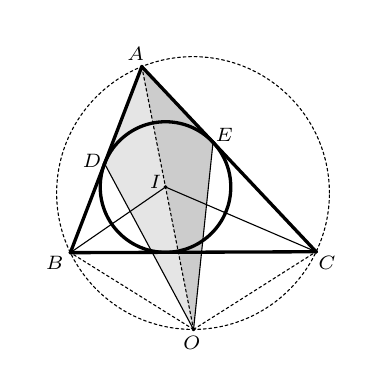
\begin{tikzpicture}[line cap=round,line join=round,>=triangle 45,x=1.0cm,y=1.0cm]
		\clip(-2.1,-2.1) rectangle (2.1,2.1);
		\fill[line width=2.pt,fill=black,fill opacity=0.10000000149011612] (-0.6504635672836612,1.605271674090281) -- (-1.1234732259855378,0.3734601959721691) -- (0.006462414177680287,-1.7320387516458735) -- cycle;
		\fill[line width=2.pt,fill=black,fill opacity=0.20000000298023224] (-0.6504635672836612,1.605271674090281) -- (0.2541152511105101,0.6446287559560773) -- (0.006462414177680287,-1.7320387516458735) -- cycle;
		\draw [line width=0.4pt,dash pattern=on 1pt off 1pt] (0.,0.) circle (1.7320508075688772cm);
		\draw [line width=1.2pt] (-0.6504635672836612,1.605271674090281)-- (-1.5576981968828558,-0.7573482207200986);
		\draw [line width=1.2pt] (-1.5576981968828558,-0.7573482207200986)-- (1.5633062367195063,-0.7457034331648841);
		\draw [line width=1.2pt] (1.5633062367195063,-0.7457034331648841)-- (-0.6504635672836612,1.605271674090281);
		\draw [line width=0.4pt] (-0.34948709377187953,0.07625325908140525)-- (-1.5576981968828558,-0.7573482207200986);
		\draw [line width=0.4pt] (-0.34948709377187953,0.07625325908140525)-- (1.5633062367195063,-0.7457034331648841);
		\draw [line width=0.4pt] (0.006462414177680287,-1.7320387516458735)-- (0.2541152511105101,0.6446287559560773);
		\draw [line width=0.4pt] (0.006462414177680287,-1.7320387516458735)-- (-1.1234732259855378,0.3734601959721691);
		\draw [line width=1.2pt] (-0.34948709377187953,0.07625325908140525) circle (0.8290877493939042cm);
		\draw [line width=0.4pt,dash pattern=on 1pt off 1pt] (-0.6504635672836612,1.605271674090281)-- (0.006462414177680287,-1.7320387516458735);
		\draw [line width=0.4pt,dash pattern=on 1pt off 1pt] (0.006462414177680287,-1.7320387516458735)-- (-1.5576981968828558,-0.7573482207200986);
		\draw [line width=0.4pt,dash pattern=on 1pt off 1pt] (0.006462414177680287,-1.7320387516458735)-- (1.5633062367195063,-0.7457034331648841);
		\begin{scriptsize}
			\draw [fill=black] (-0.6504635672836612,1.605271674090281) circle (0.5pt);
			\draw[color=black] (-0.7292280249165909,1.7614835784914809) node {$A$};
			\draw [fill=black] (-1.5576981968828558,-0.7573482207200986) circle (0.5pt);
			\draw[color=black] (-1.7576764407763594,-0.8848402109342424) node {$B$};
			\draw [fill=black] (1.5633062367195063,-0.7457034331648841) circle (0.5pt);
			\draw[color=black] (1.7016500489337711,-0.8848402109342424) node {$C$};
			\draw [fill=black] (-0.34948709377187953,0.07625325908140525) circle (0.5pt);
			\draw[color=black] (-0.4771971878284263,0.13954319142410213) node {$I$};
			\draw [fill=black] (0.006462414177680287,-1.7320387516458735) circle (0.5pt);
			\draw[color=black] (-0.013785648666317155,-1.909223613292587) node {$O$};
			\draw [fill=black] (0.2541152511105101,0.6446287559560773) circle (0.5pt);
			\draw[color=black] (0.3967807149773058,0.7371001761331365) node {$E$};
			\draw [fill=black] (-1.1234732259855378,0.3734601959721691) circle (0.5pt);
			\draw[color=black] (-1.282069861109984,0.4118990960193763) node {$D$};
		\end{scriptsize}
	\end{tikzpicture}
	\caption{}\label{fig:solution3}
\end{figure}

\switchcolumn
\textbf{证明}\quad 如图\ref{fig:solution3}所示, 因为$\angle BIC=90^\circ+\angle A/2>90^\circ$, 所以$\triangle BIC$为钝角三角形. 所以(以下结论就是\S\ref{sec:circumcenter}中“留给大家探索”的部分)
\begin{align*}
	\angle BOC&=360^\circ-2\angle BIC=360^\circ-2\left(90^\circ+\frac{\angle A}{2}\right)\\
	&=180^\circ-\angle A
\end{align*}\par
即, $\angle BOC$与$\angle BAC$互补, 我们便有$A$, $B$, $O$, $C$四点共圆. 又$BO=CO$, 所以$O$为弧$\wideparen{BC}$的中点. 所以, $AO$平分$\angle BAC$, $A, I, O$共线. 又由切线长定理, 有$AD=AE$.\par
于是, 在$\triangle DAO$与$\triangle EAO$中, 
\[DA=EA,\ \angle DAO=\angle EAO, AO=AO,\]
所以, $\triangle DAO\cong\triangle EAO$(SAS). 于是, $\angle ADO=\angle AEO$, 即$\angle ODB=\angle OEC$.\par
\textbf{注}\quad 此题为2012年中国女子数学奥林匹克试题.
\end{paracol}

\section{重心}

\begin{paracol}{2}
重心在平面几何中出现的次数少于前面介绍的内心和外心, 也少于即将介绍的垂心, 但我们先讨论重心的目的是为后面关于垂心的讨论作铺垫.\par
三角形的三条中线交于一点, 这个点就是重心. 重心最常用, 并且需要牢记的性质如下:\par

\switchcolumn*
\begin{figure}[htbp]
	\centering
	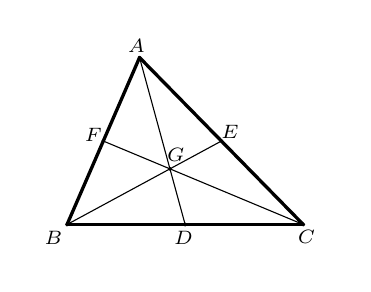
\begin{tikzpicture}[line cap=round,line join=round,>=triangle 45,x=1.0cm,y=1.0cm]
		\clip(-0.5,-0.5) rectangle (3.5,2.5);
		\draw [line width=1.2pt] (0.9207809144710447,2.1206286742151415)-- (0.,0.);
		\draw [line width=1.2pt] (0.,0.)-- (3.,0.);
		\draw [line width=1.2pt] (3.,0.)-- (0.9207809144710447,2.1206286742151415);
		\draw [line width=0.4pt] (1.5,0.)-- (0.9207809144710447,2.1206286742151415);
		\draw [line width=0.4pt] (0.,0.)-- (1.9603904572355224,1.0603143371075707);
		\draw [line width=0.4pt] (0.46039045723552235,1.0603143371075707)-- (3.,0.);
		\begin{scriptsize}
			\draw [fill=black] (0.,0.) circle (0.5pt);
			\draw[color=black] (-0.17313002507121544,-0.16392166415365703) node {$B$};
			\draw [fill=black] (3.,0.) circle (0.5pt);
			\draw[color=black] (3.041772221686424,-0.16040426563422855) node {$C$};
			\draw [fill=black] (0.9207809144710447,2.1206286742151415) circle (0.5pt);
			\draw[color=black] (0.8820895307573313,2.2701181112908517) node {$A$};
			\draw [fill=black] (0.46039045723552235,1.0603143371075707) circle (0.5pt);
			\draw[color=black] (0.33337536172648696,1.1339983895154526) node {$F$};
			\draw [fill=black] (1.9603904572355224,1.0603143371075707) circle (0.5pt);
			\draw[color=black] (2.0709702303241606,1.1762071717485942) node {$E$};
			\draw [fill=black] (1.5,0.) circle (0.5pt);
			\draw[color=black] (1.4800472790601744,-0.16392166415365703) node {$D$};
			\draw [fill=black] (1.3069269714903482,0.7068762247383804) circle (0.5pt);
			\draw[color=black] (1.3815601205161767,0.8877804931554588) node {$G$};
		\end{scriptsize}
	\end{tikzpicture}
	\caption{}\label{fig:centerofgravity}
\end{figure}

\switchcolumn
\begin{theorem}
	{\kaishu 如图\ref{fig:centerofgravity}, $\triangle ABC$的三条中线为$AD$, $BE$, $CF$, 重心为$G$, 则有
	\begin{enumerate}[(1)]
		\item $S_{\triangle AGF}=S_{\triangle FGB}=S_{\triangle BGD}=S_{\triangle GDC}=S_{\triangle EGC}=S_{\triangle AGE}$;
		\item 
		\[\frac{AG}{GD}=\frac{BG}{GE}=\frac{CG}{GF}=2.\]
	\end{enumerate}}
\end{theorem}
重心单独的性质并不丰富, 除了上述之外, 还有一些关于线段长的平方的结论, 如“重心是三角形所在平面上的到三个顶点的距离的平方和最小的点”, 我们在此就不再展开讨论, 有兴趣的同学可以自行了解.
\end{paracol}

\section{垂心}

\begin{paracol}{2}
三角形的三条高(所在直线)交于一点, 这个点被称为垂心.\par
垂心的几何结构非常丰富, 因为三条高就意味着三个垂直, 就能产生很多的四点共圆与相似三角形, 于是就有非常多的比例关系和角度关系, 下面将为大家一一介绍.\par

\switchcolumn*
\begin{figure}[htbp]
	\centering
	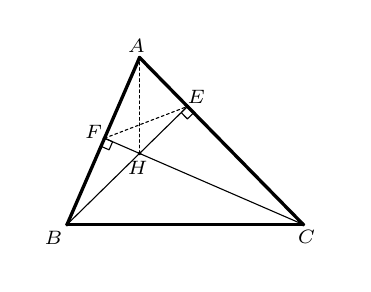
\begin{tikzpicture}[line cap=round,line join=round,>=triangle 45,x=1.0cm,y=1.0cm]
		\clip(-0.5,-0.5) rectangle (3.5,2.5);
		\draw[line width=0.4pt] (0.4312997747486718,0.9933162765867981) -- (0.5339627364331319,0.9487398276820368) -- (0.5785391853378932,1.0514027893664968) -- (0.47587622365343313,1.095979238271258) -- cycle; 
		\draw[line width=0.4pt] (1.4496585746606239,1.4213510420680464) -- (1.5280159149637722,1.3414331421994918) -- (1.6079338148323266,1.4197904825026404) -- (1.5295764745291782,1.4997083823711947) -- cycle; 
		\draw [line width=1.2pt] (0.9207809144710447,2.1206286742151415)-- (0.,0.);
		\draw [line width=1.2pt] (0.,0.)-- (3.,0.);
		\draw [line width=1.2pt] (3.,0.)-- (0.9207809144710447,2.1206286742151415);
		\draw [line width=0.4pt] (0.47587622365343313,1.095979238271258)-- (3.,0.);
		\draw [line width=0.4pt] (1.5295764745291782,1.4997083823711947)-- (0.,0.);
		\draw [line width=0.4pt,dash pattern=on 1pt off 1pt] (0.9207809144710447,0.902800794046403)-- (0.9207809144710447,2.1206286742151415);
		\draw [line width=0.4pt,dash pattern=on 1pt off 1pt] (0.47587622365343313,1.095979238271258)-- (1.5295764745291782,1.4997083823711947);
		\begin{scriptsize}
			\draw [fill=black] (0.,0.) circle (0.5pt);
			\draw[color=black] (-0.17313002507121505,-0.16392166415365864) node {$B$};
			\draw [fill=black] (3.,0.) circle (0.5pt);
			\draw[color=black] (3.0417722216864242,-0.16040426563423016) node {$C$};
			\draw [fill=black] (0.9207809144710447,2.1206286742151415) circle (0.5pt);
			\draw[color=black] (0.8820895307573317,2.2701181112908504) node {$A$};
			\draw [fill=black] (0.47587622365343313,1.095979238271258) circle (0.5pt);
			\draw[color=black] (0.33689276024591586,1.1797245702680212) node {$F$};
			\draw [fill=black] (1.5295764745291782,1.4997083823711947) circle (0.5pt);
			\draw[color=black] (1.6418476109538853,1.62291678371601) node {$E$};
			\draw [fill=black] (0.9207809144710447,0.902800794046403) circle (0.5pt);
			\draw[color=black] (0.8961591248350457,0.7224627627423187) node {$H$};
		\end{scriptsize}
	\end{tikzpicture}
	\caption{}\label{fig:orthocenter1}
\end{figure}

\switchcolumn
首先我们要证明垂心的存在性, 即三角形的三条高交于一点. 我们介绍两种证明方法. 首先是最直接的方法, 如图\ref{fig:orthocenter1}所示, 作$\triangle ABC$的两条高$BE$, $CF$, 设它们交于$H$. 我们想证明过顶点$A$的高也过$H$, 就只需证明$AH\perp BC$. 这等价于$\angle HAC+\angle ABC=90^\circ$. 又因为$\angle AFH+\angle AEH=90^\circ+90^\circ=180^\circ$, $\angle BFC=90^\circ=\angle BEC$, 所以$A$, $F$, $H$, $E$共圆, $B$, $F$, $E$, $C$共圆. 所以, $\angle CAH=\angle EFC=\angle EBC$. 又因为$\angle EBC+\angle ABC=90^\circ$, 所以$\angle CAH+\angle ABC=90^\circ$, 我们便证明了结论.\par
另一种方法则是考虑塞瓦定理. 设$\triangle ABC$的三条高为$AD$, $BE$, $CF$, 则
\begin{align*}
AE=AB\cos{A},\ AF=AC\cos{A},\ BD=BA\cos{B},\\
BF=BC\cos{B},\ CD=CA\cos{C},\ CE=CB\cos{C}.
\end{align*}
于是, 
\begin{align*}
\frac{AF}{FB}\cdot\frac{BD}{DC}\cdot\frac{CE}{EA}=&\frac{AC\cos{A}}{BC\cos{B}}\cdot\frac{BA\cos{B}}{CA\cos{C}}\\
\cdot&\frac{CB\cos{C}}{AB\cos{A}}=1.
\end{align*}\par
于是, 我们便证明了三角形的三条高交于一点.\par
还有一件值得注意的事情: 如果$ H $为$ \triangle ABC $的垂心, 那么我们可以得到$ A $ 为 $ \triangle BHC $的垂心, $ B $为$ \triangle CHA $的垂心, $ C $为$ \triangle AHB $的垂心. 即, $ A $, $ B $, $ C $, $ H $四个点, 任意一个点都是余下三点组成的三角形的垂心. 我们一般称这样的四个点为“垂心组”.\par
下面我们分类介绍垂心的性质.

\subsection{有关角度的性质}\label{subsec:angle}
对于垂心, 我们有如下角度结论:

\switchcolumn*
\begin{figure}[htbp]
	\centering
	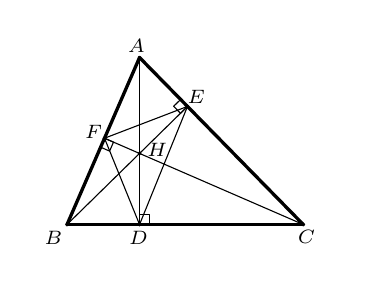
\begin{tikzpicture}[line cap=round,line join=round,>=triangle 45,x=1.0cm,y=1.0cm]
		\clip(-0.5,-0.5) rectangle (3.5,2.5);
		\draw[line width=0.4pt] (0.42634683598147616,0.9819092808440804) -- (0.5404167934086539,0.9323798931721233) -- (0.5899461810806109,1.0464498505993012) -- (0.47587622365343313,1.095979238271258) -- cycle; 
		\draw[line width=0.4pt] (1.4425127630812355,1.5885060488918108) -- (1.3537150965606195,1.501442337443868) -- (1.4407788080085622,1.412644670923252) -- (1.5295764745291782,1.4997083823711947) -- cycle; 
		\draw[line width=0.4pt] (1.045139731732215,0.) -- (1.045139731732215,0.12435881726117033) -- (0.9207809144710447,0.12435881726117033) -- (0.9207809144710447,0.) -- cycle; 
		\draw [line width=1.2pt] (0.9207809144710447,2.1206286742151415)-- (0.,0.);
		\draw [line width=1.2pt] (0.,0.)-- (3.,0.);
		\draw [line width=1.2pt] (3.,0.)-- (0.9207809144710447,2.1206286742151415);
		\draw [line width=0.4pt] (0.47587622365343313,1.095979238271258)-- (3.,0.);
		\draw [line width=0.4pt] (1.5295764745291782,1.4997083823711947)-- (0.,0.);
		\draw [line width=0.4pt] (0.47587622365343313,1.095979238271258)-- (1.5295764745291782,1.4997083823711947);
		\draw [line width=0.4pt] (0.9207809144710447,2.1206286742151415)-- (0.9207809144710447,0.);
		\draw [line width=0.4pt] (1.5295764745291782,1.4997083823711947)-- (0.9207809144710447,0.);
		\draw [line width=0.4pt] (0.9207809144710447,0.)-- (0.47587622365343313,1.095979238271258);
		\begin{scriptsize}
			\draw [fill=black] (0.,0.) circle (0.5pt);
			\draw[color=black] (-0.17313002507121464,-0.16392166415365902) node {$B$};
			\draw [fill=black] (3.,0.) circle (0.5pt);
			\draw[color=black] (3.0417722216864247,-0.16040426563423055) node {$C$};
			\draw [fill=black] (0.9207809144710447,2.1206286742151415) circle (0.5pt);
			\draw[color=black] (0.8820895307573321,2.27011811129085) node {$A$};
			\draw [fill=black] (0.47587622365343313,1.095979238271258) circle (0.5pt);
			\draw[color=black] (0.33689276024591625,1.1797245702680208) node {$F$};
			\draw [fill=black] (1.5295764745291782,1.4997083823711947) circle (0.5pt);
			\draw[color=black] (1.6418476109538858,1.6229167837160094) node {$E$};
			\draw [fill=black] (0.9207809144710447,0.902800794046403) circle (0.5pt);
			\draw[color=black] (1.1458944197144687,0.947576267985741) node {$H$};
			\draw [fill=black] (0.9207809144710447,0.) circle (0.5pt);
			\draw[color=black] (0.9067113203933315,-0.17095646119251598) node {$D$};
		\end{scriptsize}
	\end{tikzpicture}
	\caption{}\label{fig:orthocenter2}
\end{figure}

\switchcolumn
\begin{theorem}
	\kaishu 如图\ref{fig:orthocenter2}, 我们有:
	\begin{enumerate}[(1)]
		\item $\angle BHC=180^\circ-\angle BAC$, $\angle CHA=180^\circ-\angle CBA$, $\angle AHB=180^\circ-\angle ACB$.
		\item $\angle FBH=\angle FDH=\angle EDH=\angle ECH=90^\circ-\angle A$, 其余类似; 特别地, $DH$平分$\angle EDF$, 结合其它两个类似结论可知$H$为$\triangle DEF$的内心;
		\item $\angle FDB=\angle EDC=\angle FHB=\angle EHC=\angle A$, 其余类似; 特别地, $BC$为$\angle EDF$的外角平分线, 结合其它两个类似结论可知$A$, $B$, $C$为$\triangle DEF$的三个旁心(将会在后面介绍).
	\end{enumerate}
\end{theorem}
以上结论均可由六个圆内接四边形$AEHF$, $BFHD$, $CDHE$, $BCEF$, $CAFD$, $ABDE$的角度性质得到.\par
由此, 我们会发现非常多组相似三角形, 除了六组四点共圆而产生的, 还有六组相似三角形: $\triangle ABD$ 与 $\triangle CHD$, $\triangle ACD$ 与 $\triangle BHD$, $\triangle BCE$ 与 $\triangle AHE$, $\triangle BAE$ 与 $\triangle CHE$, $\triangle CAF$ 与 $\triangle BHF$, $\triangle CBF$ 与 $\triangle AHF$.\par
以上结论不必死记硬背, 我们要做到的是, 我们知道以上列出来的角度都是可以通过$\triangle ABC$的三个内角表示和计算出来的.\par
以上结论要求大家全部掌握.

\subsection{有关边长的结论}
由\S\ref{subsec:angle}中的结论, 我们不难得到以下有关边长的结论.\par
首先是关于线段乘积的:
\begin{theorem}
\kaishu 如图\ref{fig:orthocenter2}, 
\begin{enumerate}[(1)]
	\item $AF\cdot AB=AE\cdot AC$, $BF\cdot BA=AD\cdot BC$, $CD\cdot CB=CE\cdot CA$;
	\item $AH\cdot HD=BH\cdot HE=CH\cdot HF$;
	\item $DH\cdot DA=DB\cdot BC$, $EH\cdot EB=EA\cdot EC$, $FH\cdot FC=FA\cdot FB$.
\end{enumerate}
\end{theorem}\par
(1)与(2)都可以由四点共圆直接得到, (3)只需注意到\S\ref{subsec:angle}中单独列出的六组相似三角形.\par
另外还有还有一组关系:
\begin{theorem}
\kaishu 如图\ref{fig:orthocenter2}, 
\[BC=AH\tan{A},\ CA=BH\tan{B},\ AB=CH\tan{C}.\]
\end{theorem}\par
只需注意到$\triangle AEH\sim\triangle BEC$, 所以
\[\frac{BC}{AH}=\frac{BE}{AE}=\tan{A}.\]\par
同样, 同学们不必死记硬背这些结论, 思考与理解其本质在任何时候都是最重要的.\par
以上结论, 由四点共圆可以直接导出的要求大家全部掌握, 余下的两个结论也很有用, 希望大家熟记.

\subsection{垂心的对称性质}
以下内容大家可以作为兴趣了解, 对此不做要求.\par
本小节我们会重点探讨垂心关于三边的对称点, 与垂心关于三边中点的中心对称点. 这些结论大多都与外心有关. 这几个结构中都有着极为丰富的几何性质.\par
首先我们了解一下垂心关于三边的对称点.\par

\switchcolumn*
\begin{figure}[htbp]
	\centering
	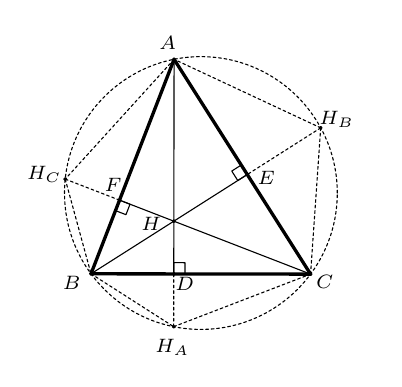
\begin{tikzpicture}[line cap=round,line join=round,>=triangle 45,x=1.0cm,y=1.0cm]
		\clip(-2.2,-2.1) rectangle (2.2,2.1);
		\draw[line width=0.4pt] (0.5123693251943633,0.35561363795704093) -- (0.39188840134350045,0.2790638594620835) -- (0.46843817983845787,0.15858293561122075) -- (0.5889191036893207,0.23513271410617814) -- cycle; 
		\draw[line width=0.4pt] (-0.2018940889794766,-1.02751756513209) -- (-0.20168675882034717,-0.8847748643947508) -- (-0.3444294595576863,-0.8845675342356215) -- (-0.3446367897168157,-1.0273102349729606) -- cycle; 
		\draw[line width=0.4pt] (-1.0848847026880362,-0.2234157541125335) -- (-0.9517754161618235,-0.2749661124048584) -- (-0.9002250578694986,-0.14185682587864576) -- (-1.0333343443957113,-0.09030646758632088) -- cycle; 
		\draw [line width=0.4pt,dash pattern=on 1pt off 1pt] (0.,0.) circle (1.7320508075688772cm);
		\draw [line width=1.2pt] (-0.3406780314770083,1.6982162638689309)-- (-1.3956245185968719,-1.0257837019036955);
		\draw [line width=1.2pt] (-1.3956245185968719,-1.0257837019036955)-- (1.3926387865296932,-1.0298335837663788);
		\draw [line width=1.2pt] (1.3926387865296932,-1.0298335837663788)-- (-0.3406780314770083,1.6982162638689309);
		\draw [line width=0.4pt] (-0.3406780314770083,1.6982162638689309)-- (-0.3446367897168157,-1.0273102349729606);
		\draw [line width=0.4pt] (-1.3956245185968719,-1.0257837019036955)-- (0.5889191036893207,0.23513271410617814);
		\draw [line width=0.4pt] (1.3926387865296932,-1.0298335837663788)-- (-1.0333343443957113,-0.09030646758632088);
		\draw [line width=0.4pt,dash pattern=on 1pt off 1pt] (-1.0333343443957113,-0.09030646758632088)-- (-1.7230049252472361,0.17678808662850182);
		\draw [line width=0.4pt,dash pattern=on 1pt off 1pt] (-1.7230049252472361,0.17678808662850182)-- (-1.3956245185968719,-1.0257837019036955);
		\draw [line width=0.4pt,dash pattern=on 1pt off 1pt] (-1.3956245185968719,-1.0257837019036955)-- (-0.3456098158894446,-1.697219448144778);
		\draw [line width=0.4pt,dash pattern=on 1pt off 1pt] (-0.3456098158894446,-1.697219448144778)-- (-0.3446367897168157,-1.0273102349729606);
		\draw [line width=0.4pt,dash pattern=on 1pt off 1pt] (-0.3456098158894446,-1.697219448144778)-- (1.3926387865296932,-1.0298335837663788);
		\draw [line width=0.4pt,dash pattern=on 1pt off 1pt] (1.5215019709228281,0.8276664500134996)-- (0.5889191036893207,0.23513271410617814);
		\draw [line width=0.4pt,dash pattern=on 1pt off 1pt] (1.5215019709228281,0.8276664500134996)-- (-0.3406780314770083,1.6982162638689309);
		\draw [line width=0.4pt,dash pattern=on 1pt off 1pt] (1.5215019709228281,0.8276664500134996)-- (1.3926387865296932,-1.0298335837663788);
		\draw [line width=0.4pt,dash pattern=on 1pt off 1pt] (-0.3406780314770083,1.6982162638689309)-- (-1.7230049252472361,0.17678808662850182);
		\begin{scriptsize}
			\draw [fill=black] (-0.3406780314770083,1.6982162638689309) circle (0.5pt);
			\draw[color=black] (-0.42091330105353886,1.90558249921057) node {$A$};
			\draw [fill=black] (-1.3956245185968719,-1.0257837019036955) circle (0.5pt);
			\draw[color=black] (-1.6402013136144757,-1.142637532191769) node {$B$};
			\draw [fill=black] (1.3926387865296932,-1.0298335837663788) circle (0.5pt);
			\draw[color=black] (1.5735511963143514,-1.126488022091624) node {$C$};
			\draw [fill=black] (-0.3446367897168157,-1.0273102349729606) circle (0.5pt);
			\draw[color=black] (-0.2069322922266194,-1.1547496647668776) node {$D$};
			\draw [fill=black] (0.5889191036893207,0.23513271410617814) circle (0.5pt);
			\draw[color=black] (0.8306737317076879,0.18969705107018064) node {$E$};
			\draw [fill=black] (-1.0333343443957113,-0.09030646758632088) circle (0.5pt);
			\draw[color=black] (-1.115342235359768,0.10087474551938398) node {$F$};
			\draw [fill=black] (-0.3456098158894446,-1.697219448144778) circle (0.5pt);
			\draw[color=black] (-0.36237132694051366,-1.964243858536638) node {$H_A$};
			\draw [fill=black] (1.5215019709228281,0.8276664500134996) circle (0.5pt);
			\draw[color=black] (1.7249528535032095,0.9305558269143253) node {$H_B$};
			\draw [fill=black] (-0.34366376354418676,-0.3574010218011434) circle (0.5pt);
			\draw[color=black] (-0.630856932355422,-0.3876479350099975) node {$H$};
			\draw [fill=black] (-1.7230049252472361,0.17678808662850182) circle (0.5pt);
			\draw[color=black] (-1.9894344695301085,0.24016427013313324) node {$H_C$};
		\end{scriptsize}
	\end{tikzpicture}
	\caption{}\label{fig:orthocenter3}
\end{figure}

\switchcolumn
如图\ref{fig:orthocenter3}, 作$H$关于$BC$, $CA$, $AB$的对称点$H_A$, $H_B$, $H_C$. 我们先来研究$H_A$. 由于对称, 我们有
\[\angle B H_A C=\angle BHC.\]
于是,
\[\angle BAC+\angle B H_A C=\angle BAC+\angle BHC=180^\circ.\]\par
所以, $H_A$就在$\triangle ABC$的外接圆上.\par
同理, $H_B$, $H_C$也在$\triangle ABC$的外接圆上.\par
我们又注意到, 由于对称, 我们有
\[AH_C=AH=AH_B,\ BH_A=BH=BH_C,\ CH_A=CH=CH_B,\]
所以, 三条直线$BC$, $CA$, $AB$分别是$HH_A$, $HH_B$, $HH_C$的垂直平分线. 而且, 我们还会注意到$H$为$\triangle H_AH_BH_C$的内心(想一想为什么), 所以这里的三组线段相等也可以看做鸡爪定理.\par
由上面的讨论, 我们可以发现, 由于$ \triangle BHC $和$ \triangle BH_AC $关于$ BC $对称, 所以它们全等, 那么它们的外接圆是等圆(半径相等的圆). 又$ \triangle BH_AC $的外接圆就是$ \triangle ABC $的外接圆, 所以我们可以说, $ \triangle ABC $的外接圆与$ \triangle BHC $的外接圆为等圆. 同理, 我们可以说, $ \triangle ABC $, $ \triangle BHC $, $ \triangle CHA $与$ \triangle AHB $的外接圆均为等圆. 我们也可以说: 过一个垂心组的任意三点所形成的四个圆都为等圆.\par 
我们再来看看垂心关于三边中点的对称点. 这次我们只画出一组.

\switchcolumn*
\begin{figure}[htbp]
	\centering
	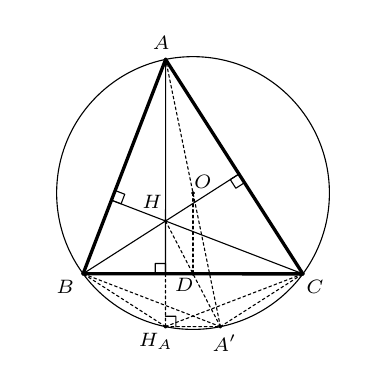
\begin{tikzpicture}[line cap=round,line join=round,>=triangle 45,x=1.0cm,y=1.0cm]
		\clip(-2.1,-2.1) rectangle (2.1,2.1);
		\draw[line width=0.4pt] (-0.3492620574632669,-0.8948266436918455) -- (-0.48022561785062234,-0.8947622870787547) -- (-0.480289974463713,-1.0257258474661102) -- (-0.3493264140763576,-1.0257902040792009) -- cycle; 
		\draw[line width=0.4pt] (-0.9139281911010141,-0.13768397541842375) -- (-0.8668726696897802,-0.015465989034164268) -- (-0.9890906560740397,0.03158953237706967) -- (-1.0361461774852736,-0.09062845400718983) -- cycle; 
		\draw[line width=0.4pt] (0.4730487250354263,0.17092355867681458) -- (0.543645532946237,0.06061694507676682) -- (0.6539521465462846,0.13121375298757743) -- (0.5833553386354741,0.2415203665876252) -- cycle; 
		\draw[line width=0.4pt] (-0.2186923924049125,-1.6964548525417054) -- (-0.21862803579182166,-1.5654912921543498) -- (-0.34959159617917707,-1.5654269355412591) ; 
		\draw [line width=0.4pt] (0.,0.) circle (1.7320508075688772cm);
		\draw [line width=1.2pt] (-0.347988542741504,1.6967333243973974)-- (-1.3959976393506197,-1.0252758608918366);
		\draw [line width=1.2pt] (-1.3959976393506197,-1.0252758608918366)-- (1.3949893067316765,-1.0266473757353478);
		\draw [line width=1.2pt] (1.3949893067316765,-1.0266473757353478)-- (-0.347988542741504,1.6967333243973974);
		\draw [line width=0.4pt,dash pattern=on 1pt off 1pt] (0.34798854274150415,-1.6967333243973979)-- (-0.3489968753604472,-0.35518991222978685);
		\draw [line width=0.4pt,dash pattern=on 1pt off 1pt] (0.34798854274150415,-1.6967333243973979)-- (-0.347988542741504,1.6967333243973974);
		\draw [line width=0.4pt,dash pattern=on 1pt off 1pt] (-0.3496559527922679,-1.6963904959286145)-- (0.34798854274150415,-1.6967333243973979);
		\draw [line width=0.4pt] (-1.0361461774852736,-0.09062845400718983)-- (1.3949893067316765,-1.0266473757353478);
		\draw [line width=0.4pt] (-1.3959976393506197,-1.0252758608918366)-- (0.5833553386354741,0.2415203665876252);
		\draw [line width=0.4pt] (-0.347988542741504,1.6967333243973974)-- (-0.3493264140763576,-1.0257902040792009);
		\draw [line width=0.4pt,dash pattern=on 1pt off 1pt] (-0.3493264140763576,-1.0257902040792009)-- (-0.3496559527922679,-1.6963904959286145);
		\draw [line width=0.4pt,dash pattern=on 1pt off 1pt] (-0.3496559527922679,-1.6963904959286145)-- (-1.3959976393506197,-1.0252758608918366);
		\draw [line width=0.4pt,dash pattern=on 1pt off 1pt] (-0.3496559527922679,-1.6963904959286145)-- (1.3949893067316765,-1.0266473757353478);
		\draw [line width=0.4pt,dash pattern=on 1pt off 1pt] (0.34798854274150415,-1.6967333243973979)-- (1.3949893067316765,-1.0266473757353478);
		\draw [line width=0.4pt,dash pattern=on 1pt off 1pt] (0.34798854274150415,-1.6967333243973979)-- (-1.3959976393506197,-1.0252758608918366);
		\begin{scriptsize}
			\draw [fill=black] (-0.347988542741504,1.6967333243973974) circle (0.5pt);
			\draw[color=black] (-0.40486208050308337,1.9090476853928322) node {$A$};
			\draw [fill=black] (-1.3959976393506197,-1.0252758608918366) circle (0.5pt);
			\draw[color=black] (-1.6231353655951204,-1.1901407729663631) node {$B$};
			\draw [fill=black] (1.3949893067316765,-1.0266473757353478) circle (0.5pt);
			\draw[color=black] (1.550137279019611,-1.1942565610916742) node {$C$};
			\draw [fill=black] (-0.3489968753604472,-0.35518991222978685) circle (0.5pt);
			\draw[color=black] (-0.5201041480117896,-0.11180428413487681) node {$H$};
			\draw [fill=black] (0.,0.) circle (0.5pt);
			\draw[color=black] (0.1260745876620273,0.1392587915090952) node {$O$};
			\draw [fill=black] (-5.041663094715876E-4,-1.0259616183135922) circle (0.5pt);
			\draw[color=black] (-0.11264112360600695,-1.169561832339808) node {$D$};
			\draw [fill=black] (0.34798854274150415,-1.6967333243973979) circle (0.5pt);
			\draw[color=black] (0.40183239205786003,-1.9062879067704799) node {$A'$};
			\draw [fill=black] (-0.3496559527922679,-1.6963904959286145) circle (0.5pt);
			\draw[color=black] (-0.47277258457071386,-1.8877668602065802) node {$H_A$};
			\draw [line width=0.4pt,dash pattern=on 1pt off 1pt] (0.,0.)-- (0.,-1.026);
		\end{scriptsize}
	\end{tikzpicture}
	\caption{}\label{fig:orthocenter4}
\end{figure}

\switchcolumn
如图\ref{fig:orthocenter4}, 设$BC$的中点为$D$, 作$H$关于$D$的对称点$A'$, 则四边形$HBA'C$为平行四边形. 于是, $\angle CA'B=\angle BHC$, 类似于垂心关于边的对称点的性质, $A'$也在$\triangle ABC$的外接圆上.\par
而且, 如果我们把$H$关于$BC$对称点$H_A$画出来, 那么$\triangle H_A BC\cong\triangle HBC\cong\triangle A'CB$, 于是$BH_AA'C$为等腰梯形. 又由于$BC\perp AH_A$, 所以$\angle AH_AA'=90^\circ$, 即$AA'$为$\triangle ABC$的外接圆的直径.\footnote{此时, 我们会说$A'$为$A$的对径点. 这也是为什么要把这个点记为$A'$的原因之一.} 于是我们得到了一个很重要的结论:
\[\angle ABH=\angle CAO.\]\par
此时, 我们可以说, (射线)$AH$和(射线)$AO$是$\angle BAC$的一组等角线, 也可以说(射线)$AH$和(射线)$AO$关于$\angle BAC$的内角平分线对称. 当然, 我们也可以通过
\[\angle BAH=90^\circ-\angle ABC=\angle OAC\]
来证明这一点.\par
并且, 我们也能发现, $O$, $D$分别是$A'A$, $A'H$的中点, 所以$OD$为$\triangle AHA'$的中位线, 于是
\[AH=2OD.\]
用一句话概括, 就是\textbf{顶点到垂心的距离, 等于外心到对边的距离的二倍.}\par
总的来说, 我们上面介绍的两个结果, 即$H_A$和$A'$及其相关结构, 是两个非常对称的结构.\par
我们列举一道例题来加深大家对这种对称性的感觉:

\switchcolumn*
\begin{figure}[htbp]
	\centering
	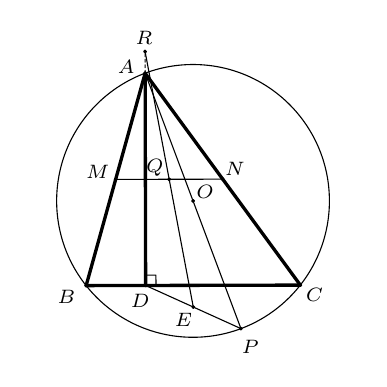
\begin{tikzpicture}[line cap=round,line join=round,>=triangle 45,x=1.0cm,y=1.0cm]
	\clip(-2.1,-2.) rectangle (2.1,2.2);
		\draw[line width=0.4pt] (-0.47075444299543057,-1.0736884430639855) -- (-0.47106531783172745,-0.9426759383699816) -- (-0.6020778225257314,-0.9429868132062785) -- (-0.6017669476894345,-1.0739993179002825) -- cycle; 
		\draw [line width=0.4pt] (0.,0.) circle (1.7320508075688772cm);
		\draw [line width=1.2pt] (-0.6081636405595375,1.621769708158766)-- (-1.3574500367986515,-1.0757924509845471);
		\draw [line width=1.2pt] (-1.3574500367986515,-1.0757924509845471)-- (1.3625401399748682,-1.0693382846215065);
		\draw [line width=1.2pt] (1.3625401399748682,-1.0693382846215065)-- (-0.6081636405595375,1.621769708158766);
		\draw [line width=1.2pt] (-0.6017669476894345,-1.0739993179002825)-- (-0.6081636405595375,1.621769708158766);
		\draw [line width=0.4pt] (-0.6081636405595375,1.621769708158766)-- (0.6081636405595375,-1.621769708158766);
		\draw [line width=0.4pt] (0.6081636405595375,-1.621769708158766)-- (-0.6017669476894345,-1.0739993179002825);
		\draw [line width=0.4pt] (-0.9828068386790945,0.2729886285871095)-- (0.37718824970766535,0.2762157117686298);
		\draw [line width=0.4pt,dash pattern=on 1pt off 1pt] (-0.6081636405595375,1.621769708158766)-- (-0.6088169354064807,1.8970888533852637);
		\draw [line width=0.4pt] (0.0031983464350515134,-1.3478845130295243)-- (-0.6088169354064807,1.8970888533852637);
		\begin{scriptsize}
			\draw [fill=black] (-0.6081636405595375,1.621769708158766) circle (0.5pt);
			\draw[color=black] (-0.8487411222917558,1.6999102252192304) node {$A$};
			\draw [fill=black] (-1.3574500367986515,-1.0757924509845471) circle (0.5pt);
			\draw[color=black] (-1.6063312021947518,-1.2151646474509985) node {$B$};
			\draw [fill=black] (1.3625401399748682,-1.0693382846215065) circle (0.5pt);
			\draw[color=black] (1.5434319017497697,-1.1986952978878898) node {$C$};
			\draw [fill=black] (-0.6017669476894345,-1.0739993179002825) circle (0.5pt);
			\draw[color=black] (-0.6716956144883383,-1.2645726961403243) node {$D$};
			\draw [fill=black] (0.,0.) circle (0.5pt);
			\draw[color=black] (0.15177186366709217,0.11885266716080127) node {$O$};
			\draw [fill=black] (0.6081636405595375,-1.621769708158766) circle (0.5pt);
			\draw[color=black] (0.7281990983758936,-1.8574692804122352) node {$P$};
			\draw [fill=black] (-0.9828068386790945,0.2729886285871095) circle (0.5pt);
			\draw[color=black] (-1.2110668126801452,0.370010247998208) node {$M$};
			\draw [fill=black] (0.37718824970766535,0.2762157117686298) circle (0.5pt);
			\draw[color=black] (0.5305669036185903,0.40294894712442525) node {$N$};
			\draw [fill=black] (-0.3028092944857146,0.27460217017786964) circle (0.5pt);
			\draw[color=black] (-0.48641543190336645,0.41530095929675676) node {$Q$};
			\draw [fill=black] (0.0031983464350515134,-1.3478845130295243) circle (0.5pt);
			\draw[color=black] (-0.11997240412419988,-1.511612939586954) node {$E$};
			\draw [fill=black] (-0.6088169354064807,1.8970888533852637) circle (0.5pt);
			\draw[color=black] (-0.6222875657990125,2.0663532529983977) node {$R$};
		\end{scriptsize}
	\end{tikzpicture}
	\caption{}\label{fig:example4}
\end{figure}

\switchcolumn
\begin{tcolorbox}
	\textbf{例}\quad {\kaishu 如图\ref{fig:example4}, $\triangle ABC$的外接圆为$\odot O$, 其中一条高为$AD$. 延长 $AO$ 交 $\odot O$ 于$P$, 连接$DE$, 取其中点$E$. $M$, $N$分别为$AB$, $AC$的中点, 连接$MN$, 取其中点$Q$. 连接并延长$EQ$至$R$使得$RQ=EQ$. 求证: $R$在直线$AD$上.}
\end{tcolorbox}\par
\textbf{分析}\quad 首先, 我们一眼就能发现$P$为$A$的对径点, 所以我们可以联想到上面说的对称性. 根据前面的讨论, 我们可以知道$D$和$P$在“水平方向上”(此处指沿$BC$的方向)是关于$BC$中点对称的. 而$E$为$DP$的中点, 所以我们可以得到$E$与 $BC$ 中点在水平方向上是一样的. 而$Q$为$MN$中点, 我们也能比较方便地刻画 $M$ 和 $N$ 的水平位置(分别为$B$和$A$的水平位置的中点, 和$C$和$A$的水平位置的中点), 也能比较好地刻画$Q$在水平位置上的位置. 加上$Q$为$ER$中点, 有了$E$和$Q$的水平位置, 就不难知道$R$的水平位置, 结论就不难证明.\par
我们可以注意到, 思考这道题的方法主要是考虑点的水平位置. 如果建立了以直线$BC$为$x$轴的平面直角坐标系, 那么就是考虑坐标的水平分量. 由于题目要求证明的是$R$在直线$AD$上, 那么只需要证明$R$的水平位置和$A$(或$D$)的水平位置相同.\par
当然, 上面的思考过程是不够严谨的, 下面我们来看一下这道题的解法, 探究一下“考虑水平位置”的思想是如何运用到解题当中的.\par

\switchcolumn*
\begin{figure}[htbp]
	\centering
	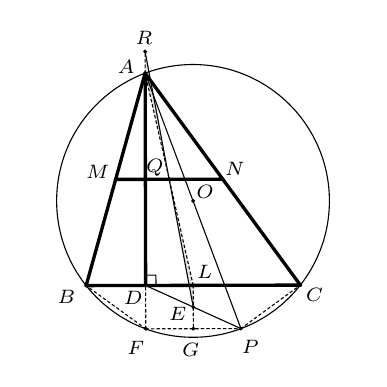
\begin{tikzpicture}[line cap=round,line join=round,>=triangle 45,x=1.0cm,y=1.0cm]
		\clip(-2.1,-2.) rectangle (2.1,2.2);
		\draw[line width=0.4pt] (-0.47075444299543057,-1.0736884430639855) -- (-0.47106531783172745,-0.9426759383699816) -- (-0.6020778225257314,-0.9429868132062785) -- (-0.6017669476894345,-1.0739993179002825) -- cycle; 
		\fill[line width=2.pt,fill=black,fill opacity=0.10000000149011612] (-0.6088169354064807,1.8970888533852637) -- (-0.6081636405595375,1.621769708158766) -- (-0.3028092944857146,0.27460217017786964) -- cycle;
		\fill[line width=2.pt,fill=black,fill opacity=0.10000000149011612] (-0.3028092944857146,0.27460217017786964) -- (0.00254505158810836,-1.0725653678030267) -- (0.0031983464350515134,-1.3478845130295243) -- cycle;
		\draw [line width=0.4pt] (0.,0.) circle (1.7320508075688772cm);
		\draw [line width=1.2pt] (-0.6081636405595375,1.621769708158766)-- (-1.3574500367986515,-1.0757924509845471);
		\draw [line width=1.2pt] (-1.3574500367986515,-1.0757924509845471)-- (1.3625401399748682,-1.0693382846215065);
		\draw [line width=1.2pt] (1.3625401399748682,-1.0693382846215065)-- (-0.6081636405595375,1.621769708158766);
		\draw [line width=1.2pt] (-0.6017669476894345,-1.0739993179002825)-- (-0.6081636405595375,1.621769708158766);
		\draw [line width=0.4pt] (-0.6081636405595375,1.621769708158766)-- (0.6081636405595375,-1.621769708158766);
		\draw [line width=0.4pt] (0.6081636405595375,-1.621769708158766)-- (-0.6017669476894345,-1.0739993179002825);
		\draw [line width=1.2pt] (-0.9828068386790945,0.2729886285871095)-- (0.37718824970766535,0.2762157117686298);
		\draw [line width=0.4pt,dash pattern=on 1pt off 1pt] (-0.6081636405595375,1.621769708158766)-- (-0.6088169354064807,1.8970888533852637);
		\draw [line width=0.4pt] (0.0031983464350515134,-1.3478845130295243)-- (-0.6088169354064807,1.8970888533852637);
		\draw [line width=0.4pt,dash pattern=on 1pt off 1pt] (-0.6004603579955483,-1.6246376083532774)-- (-0.6017669476894345,-1.0739993179002825);
		\draw [line width=0.4pt,dash pattern=on 1pt off 1pt] (-0.6004603579955483,-1.6246376083532774)-- (-1.3574500367986515,-1.0757924509845471);
		\draw [line width=0.4pt,dash pattern=on 1pt off 1pt] (-0.6004603579955483,-1.6246376083532774)-- (0.6081636405595375,-1.621769708158766);
		\draw [line width=0.4pt,dash pattern=on 1pt off 1pt] (0.6081636405595375,-1.621769708158766)-- (1.3625401399748682,-1.0693382846215065);
		\draw [line width=0.4pt,dash pattern=on 1pt off 1pt] (0.00254505158810836,-1.0725653678030267)-- (0.003851641281994611,-1.6232036582560219);
		\draw [line width=0.4pt,dash pattern=on 1pt off 1pt] (0.00254505158810836,-1.0725653678030267)-- (-0.6081636405595375,1.621769708158766);
		\begin{scriptsize}
			\draw [fill=black] (-0.6081636405595375,1.621769708158766) circle (0.5pt);
			\draw[color=black] (-0.8487411222917558,1.6999102252192304) node {$A$};
			\draw [fill=black] (-1.3574500367986515,-1.0757924509845471) circle (0.5pt);
			\draw[color=black] (-1.6063312021947518,-1.2151646474509985) node {$B$};
			\draw [fill=black] (1.3625401399748682,-1.0693382846215065) circle (0.5pt);
			\draw[color=black] (1.5434319017497697,-1.1986952978878898) node {$C$};
			\draw [fill=black] (-0.6017669476894345,-1.0739993179002825) circle (0.5pt);
			\draw[color=black] (-0.7581596996946585,-1.2357513344048843) node {$D$};
			\draw [fill=black] (0.,0.) circle (0.5pt);
			\draw[color=black] (0.15177186366709217,0.11885266716080127) node {$O$};
			\draw [fill=black] (0.6081636405595375,-1.621769708158766) circle (0.5pt);
			\draw[color=black] (0.7281990983758936,-1.8574692804122352) node {$P$};
			\draw [fill=black] (-0.9828068386790945,0.2729886285871095) circle (0.5pt);
			\draw[color=black] (-1.2110668126801452,0.370010247998208) node {$M$};
			\draw [fill=black] (0.37718824970766535,0.2762157117686298) circle (0.5pt);
			\draw[color=black] (0.5305669036185903,0.40294894712442525) node {$N$};
			\draw [fill=black] (-0.3028092944857146,0.27460217017786964) circle (0.5pt);
			\draw[color=black] (-0.48641543190336645,0.41530095929675676) node {$Q$};
			\draw [fill=black] (0.0031983464350515134,-1.3478845130295243) circle (0.5pt);
			\draw[color=black] (-0.19408447715818863,-1.437500866552965) node {$E$};
			\draw [fill=black] (-0.6088169354064807,1.8970888533852637) circle (0.5pt);
			\draw[color=black] (-0.6222875657990125,2.0663532529983977) node {$R$};
			\draw [fill=black] (0.00254505158810836,-1.0725653678030267) circle (0.5pt);
			\draw[color=black] (0.14765452627631503,-0.898129668361157) node {$L$};
			\draw [fill=black] (-0.6004603579955483,-1.6246376083532774) circle (0.5pt);
			\draw[color=black] (-0.7252210005684412,-1.8698212925845668) node {$F$};
			\draw [fill=black] (0.003851641281994611,-1.6232036582560219) circle (0.5pt);
			\draw[color=black] (-0.029390981527102525,-1.8945253169292298) node {$G$};
		\end{scriptsize}
	\end{tikzpicture}
	\caption{}\label{fig:solution4}
\end{figure}

\switchcolumn
\textbf{解}\quad 如图, 延长$AD$交$\odot O$于另一点$F$. 取$FP$, $BC$中点$G$, $L$并连接$EG$, $EL$. 连接$AL$, $BF$, $PC$.\par
由于
\[\angle BAF=90^\circ-\angle B=\angle CAP,\]
我们可以得到$BF=CP$. 由此可以得到$BFPC$为等腰梯形(这里用到一个结论: 有一组对边相等的圆内接四边形为矩形或等腰梯形, 想一想为什么). 于是, 由于$L$, $G$为$BC$, $PF$的中点, 所以
\[LG\perp FP.\]
又由于$EG$为$\triangle DPF$的中位线, 而且$\angle DFP=90^\circ$, 所以
\[EG\perp FP.\]

\switchcolumn*
{\kaishu 在这里, 我们实际上说明了$E$的水平位置就是$BC$的中\\点.}

\switchcolumn
结合$LG\perp FP$, 得到$L$, $E$, $G$共线, 直线$LEG$垂直于$BC$, 于是$EL\parallel AD$.\par
容易得到$A$, $Q$, $L$共线, 并且$Q$为$AL$的中点(这可以由位似或中位线证明). 所以$AQ=LQ$. 又$RQ=EQ$, 所以, 在$\triangle AQR$与$\triangle LQE$中,
\[QA=QL,\ \angle AQR=\angle LQE,\ QR=QE,\]
所以$\triangle AQR\cong\triangle LQE$(SAS). 所以$\angle QAR=\angle QLE$. 
\switchcolumn*
{\kaishu 其实我们在这里本质上说明了 $AR\parallel EL$, 于是 $AR\perp BC$, 即$R$和$A$在水平方向上的位置相同.}
\switchcolumn
又由于平行线的性质, 有$\angle DAL+\angle ALE=180^\circ$, 所以
\[\angle DAL+\angle LAR=180^\circ.\]
我们便证明了$R$在直线$AD$上.\par
\textbf{注1}\quad 我们可以看到, 解答中给出的方法不同于思考的思路(即“分析”中的内容), 但大体上是一致的. 在这里我们也想强调, 在这个题中我们对点的刻画方式帮助了我们解题. 题目中有很多的中点, 并且还有前文提到的对称结构, 这让我们联想到通过“水平位置”去考虑问题. \par
\textbf{注2}\quad 我们可以注意到, 这个题中并没有出现垂心, 只是出现了一条三角形的高$AD$. 但这并不妨碍我们使用前文提到的对称结构. 这说明了这个对称的结构应用很广泛, 其本质就是$AH$, $AO$为$\angle BAC$的一组等角线, 其中$H$为$\triangle ABC$的垂心. 而$H$关于$BC$和$BC$中点的对应点又恰好是直线$AH$和直线$AO$与$\odot O$的另一个交点. 顺便提一下, 我们说一个几何图形的结构很丰富, 一般来说是这个结构中的某个点有很多种刻画方式, 如\S\ref{sec:circumcenter}中例题的“注”中所写.\par
我们可以看看垂心(下面记为$H$)关于边的中点(在这道题中是$L$)的对称点(在这道题中是$P$)到底有几种刻画方式. 首先, 它是$H$关于$L$的对称点, 这实际上已经相当于两个刻画条件了(正如\S\ref{sec:circumcenter}中例题的“注”中所写, 一般指的刻画方式为基本的数量关系或其他, 而不是像“$P$为$H$关于$L$的对称点”这种对于$P$的刻画). 而$P$还在$\odot O$上, 于是有了第三个刻画: $P$在$\odot O$上. 另外, $P$还在直线$AO$上, 这即为第四个刻画.\par
所以我们可以看到, 对于$P$, 我们就已经有了四个刻画, 这足以说明$P$的性质很丰富. 对于题目中的$F$有完全类似的结论, 大家不妨自己分析一下.\par
\textbf{注3}\quad 这道题原来为一道高中数学联赛模拟题, 被笔者修改后难度降低了不少, 解答也是笔者给出的.

\subsection{九点圆与欧拉线}
本节我们继续深入研究垂心的性质, 探讨其与外心和重心的联系, 再介绍九点圆与欧拉线的概念. 本节内容较难, 对大家不做要求.\par

\switchcolumn*
\begin{figure}[htbp]
	\centering
	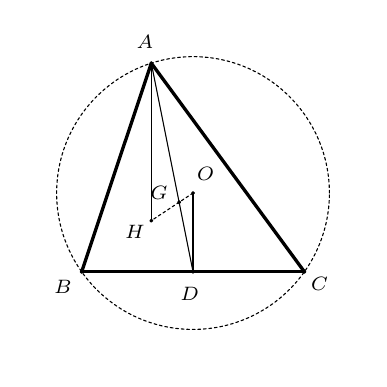
\begin{tikzpicture}[line cap=round,line join=round,>=triangle 45,x=1.0cm,y=1.0cm]
		\clip(-2.1,-2.1) rectangle (2.1,2.1);
		\draw [line width=0.4pt,dash pattern=on 1pt off 1pt] (0.,0.) circle (1.7320508075688772cm);
		\draw [line width=1.2pt] (-0.5297363809567105,1.6490540824032687)-- (-1.4142135736923451,-0.9999999839921626);
		\draw [line width=1.2pt] (-1.4142135736923451,-0.9999999839921626)-- (1.4142135687335498,-0.9999999910049585);
		\draw [line width=1.2pt] (1.4142135687335498,-0.9999999910049585)-- (-0.5297363809567105,1.6490540824032687);
		\draw [line width=0.4pt] (-2.479397687160656E-9,-0.9999999874985606)-- (-0.5297363809567105,1.6490540824032687);
		\draw [line width=0.4pt,dash pattern=on 1pt off 1pt] (0.,0.)-- (-0.529736385915506,-0.35094589259385234);
		\draw [line width=0.4pt] (-2.479397687160656E-9,-0.9999999874985606)-- (0.,0.);
		\draw [line width=0.4pt] (-0.529736385915506,-0.35094589259385234)-- (-0.5297363809567105,1.6490540824032687);
		\begin{scriptsize}
			\draw [fill=black] (-0.5297363809567105,1.6490540824032687) circle (0.5pt);
			\draw[color=black] (-0.6094754316512413,1.9154917496314636) node {$A$};
			\draw [fill=black] (-1.4142135736923451,-0.9999999839921626) circle (0.5pt);
			\draw[color=black] (-1.652974082022603,-1.18904652371739) node {$B$};
			\draw [fill=black] (1.4142135687335498,-0.9999999910049585) circle (0.5pt);
			\draw[color=black] (1.607310258441154,-1.1475142391240942) node {$C$};
			\draw [fill=black] (0.,0.) circle (0.5pt);
			\draw[color=black] (0.15887183329881607,0.23862575917714982) node {$O$};
			\draw [fill=black] (-0.529736385915506,-0.35094589259385234) circle (0.5pt);
			\draw[color=black] (-0.7392638210009131,-0.4933807567796869) node {$H$};
			\draw [fill=black] (-2.479397687160656E-9,-0.9999999874985606) circle (0.5pt);
			\draw[color=black] (-0.043598054086672035,-1.2824941640523053) node {$D$};
			\draw [fill=black] (-0.17657879530516865,-0.11698196419795077) circle (0.5pt);
			\draw[color=black] (-0.43296322213568755,0.005006658339861504) node {$G$};
		\end{scriptsize}
	\end{tikzpicture}
	\caption{}\label{fig:orthocenter5}
\end{figure}

\switchcolumn
首先我们来看一下重心与外心、垂心的关系. 如图\ref{fig:orthocenter5}, $D$为$BC$中点, $O$, $G$, $H$分别为$\triangle ABC$的外心, 重心, 垂心. 由以前提到过的性质, 可知$A$, $G$, $D$共线, $OD\perp BC$, 并且
\[HA=2OD, AG=2DG.\]
我们便不难得到, $H$, $G$, $O$三点共线. 这条线被称为$\triangle ABC$的“欧拉线”. 并且我们知道, 
\[\frac{OG}{GH}=\frac{1}{2}.\]
也就是说, $G$是线段$HO$上靠近$O$的一个三等分点.\par
我们再来看看$OH$的中点, 记为$V$, 它有一些神奇的性质:\par

\switchcolumn
\begin{figure}[htbp]
	\centering
	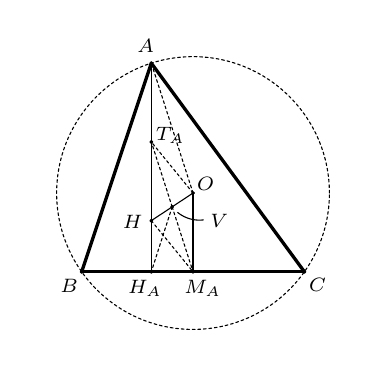
\begin{tikzpicture}[line cap=round,line join=round,>=triangle 45,x=1.0cm,y=1.0cm]
		\clip(-2.1,-2.1) rectangle (2.1,2.1);
		\draw [line width=0.4pt,dash pattern=on 1pt off 1pt] (0.,0.) circle (1.7320508075688772cm);
		\draw [line width=1.2pt] (-0.5297363809567105,1.6490540824032687)-- (-1.4142135736923451,-0.9999999839921626);
		\draw [line width=1.2pt] (-1.4142135736923451,-0.9999999839921626)-- (1.4142135687335498,-0.9999999910049585);
		\draw [line width=1.2pt] (1.4142135687335498,-0.9999999910049585)-- (-0.5297363809567105,1.6490540824032687);
		\draw [line width=0.4pt] (0.,0.)-- (-0.529736385915506,-0.35094589259385234);
		\draw [line width=0.4pt] (-2.479397687160656E-9,-0.9999999874985606)-- (0.,0.);
		\draw [line width=0.4pt] (-0.529736385915506,-0.35094589259385234)-- (-0.5297363809567105,1.6490540824032687);
		\draw [line width=0.4pt] (-0.529736385915506,-0.35094589259385234)-- (-0.5297363875247693,-0.9999999861851334);
		\draw [line width=0.4pt,dash pattern=on 1pt off 1pt] (-0.264868192957753,-0.17547294629692617)-- (-0.5297363875247693,-0.9999999861851334);
		\draw [line width=0.4pt,dash pattern=on 1pt off 1pt] (-0.264868192957753,-0.17547294629692617)-- (-0.5297363834361082,0.6490540949047081);
		\draw [line width=0.4pt,dash pattern=on 1pt off 1pt] (-0.264868192957753,-0.17547294629692617)-- (-2.479397687160656E-9,-0.9999999874985606);
		\draw [line width=0.4pt,dash pattern=on 1pt off 1pt] (0.,0.)-- (-0.5297363834361082,0.6490540949047081);
		\draw [line width=0.4pt,dash pattern=on 1pt off 1pt] (-0.529736385915506,-0.35094589259385234)-- (-2.479397687160656E-9,-0.9999999874985606);
		\draw [shift={(0.08075679049760506,0.0939288542055288)},line width=0.4pt]  plot[domain=4.030371719148535:4.82745783809623,variable=\t]({1.*0.43821679486583015*cos(\t r)+0.*0.43821679486583015*sin(\t r)},{0.*0.43821679486583015*cos(\t r)+1.*0.43821679486583015*sin(\t r)});
		\draw [line width=0.4pt,dash pattern=on 1pt off 1pt] (0.,0.)-- (-0.5297363809567105,1.6490540824032687);
		\begin{scriptsize}
			\draw [fill=black] (-0.5297363809567105,1.6490540824032687) circle (0.5pt);
			\draw[color=black] (-0.6011152036445117,1.863693591539573) node {$A$};
			\draw [fill=black] (-1.4142135736923451,-0.9999999839921626) circle (0.5pt);
			\draw[color=black] (-1.5715136753931318,-1.178064527280509) node {$B$};
			\draw [fill=black] (1.4142135687335498,-0.9999999910049585) circle (0.5pt);
			\draw[color=black] (1.5796348165032965,-1.1604209187026662) node {$C$};
			\draw [fill=black] (0.,0.) circle (0.5pt);
			\draw[color=black] (0.16108868689258635,0.1169763423331453) node {$O$};
			\draw [fill=black] (-0.529736385915506,-0.35094589259385234) circle (0.5pt);
			\draw[color=black] (-0.7669651242706395,-0.3699872544153133) node {$H$};
			\draw [fill=black] (-2.479397687160656E-9,-0.9999999874985606) circle (0.5pt);
			\draw[color=black] (0.1240371088803663,-1.2151161052939787) node {$M_A$};
			\draw [fill=black] (-0.5297363875247693,-0.9999999861851334) circle (0.5pt);
			\draw[color=black] (-0.6099370079331354,-1.2115873835784103) node {$H_A$};
			\draw [fill=black] (-0.5297363834361082,0.6490540949047081) circle (0.5pt);
			\draw[color=black] (-0.2876392706971732,0.729209559984287) node {$T_A$};
			\draw [fill=black] (-0.264868192957753,-0.17547294629692617) circle (0.5pt);
			\draw (0.12049079090887973,-0.17118891179706156) node[anchor=north west] {$V$};
		\end{scriptsize}
	\end{tikzpicture}
	\caption{}\label{fig:orthocenter6}
\end{figure}

\switchcolumn

如图\ref{fig:orthocenter6}, 我们取$BC$中点$M_A$, $A$在$BC$上的垂足$H_A$, $AH$的中点$T_A$. 同理得到$M_B$, $H_B$, $T_B$; $M_C$, $H_C$, $T_C$\par
由于$T_A$为$AH$对的中点, 所以$HT_A=AH/2=OM_A$. 又因为$HT_A\parallel OM_A$, 所以四边形$HT_AOM_A$为平行四边形. 因为平行四边形的对角线相互平分, 而 $V$ 为 $OH$ 的中点, 所以$V$也为$M_AT_A$的中点. \par
所以, $V$是$\mathrm{Rt}\triangle T_AH_AM_A$的斜边$M_AT_A$的中点. 于是, $T_AV=H_AV=M_AV$. 而在$\triangle AHO$中, $T_A$, $V$分别是$HA$, $HO$的中点, 所以$T_AV$为此三角形的中位线, 所以$T_AV=AO/2=R/2$, 其中$R$为$\odot O$的半径. 所以,
\[VT_A=VH_A=VM_A=\frac{R}{2}.\]
即, $VT_A$, $VH_A$, $VM_A$都在一个以$V$为圆心, $R/2$为半径的一个圆上.\par
同理, $VT_B$, $VH_B$, $VM_B$; $VT_C$, $VH_C$, $VM_C$都在这个园上.\par

\switchcolumn
\begin{figure}[H]
	\centering
	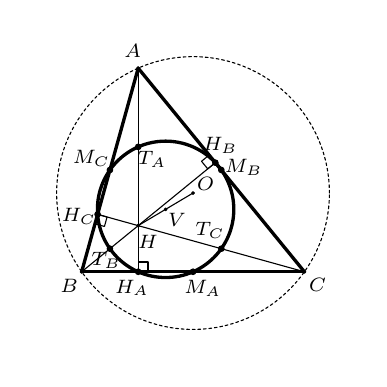
\begin{tikzpicture}[line cap=round,line join=round,>=triangle 45,x=1.0cm,y=1.0cm]
		\clip(-2.1,-2.1) rectangle (2.1,2.1);
		\draw[line width=0.4pt] (0.20451698898450754,0.4821803155565607) -- (0.10786303912631004,0.40329520822846393) -- (0.18674814645440685,0.3066412583702664) -- (0.2834020963126044,0.38552636569836324) -- cycle; 
		\draw[line width=0.4pt] (-1.2451926791746462,-0.39117639129057435) -- (-1.1249800750812822,-0.4245496739946849) -- (-1.0916067923771717,-0.3043370699013211) -- (-1.2118193964705355,-0.27096378719721054) -- cycle; 
		\draw[line width=0.4pt] (-0.5715538164102371,-0.9999999860814515) -- (-0.5715538161009095,-0.8752408333857221) -- (-0.6963129687966388,-0.8752408330763946) -- (-0.6963129691059664,-0.9999999857721239) -- cycle; 
		\draw [line width=0.4pt,dash pattern=on 1pt off 1pt] (0.,0.) circle (1.7320508075688772cm);
		\draw [line width=1.2pt] (-0.6963129626944374,1.5859218952973992)-- (-1.4142135736923451,-0.9999999839921626);
		\draw [line width=1.2pt] (-1.4142135736923451,-0.9999999839921626)-- (1.4142135687335498,-0.9999999910049585);
		\draw [line width=1.2pt] (1.4142135687335498,-0.9999999910049585)-- (-0.6963129626944374,1.5859218952973992);
		\draw [line width=0.4pt] (0.,0.)-- (-0.6963129676532328,-0.414078079699722);
		\draw [line width=0.4pt] (-0.6963129676532328,-0.414078079699722)-- (-0.6963129626944374,1.5859218952973992);
		\draw [line width=0.4pt] (-0.6963129676532328,-0.414078079699722)-- (-0.6963129691059664,-0.9999999857721239);
		\draw [line width=0.4pt] (0.2834020963126044,0.38552636569836324)-- (-0.6963129676532328,-0.414078079699722);
		\draw [line width=0.4pt] (-0.6963129676532328,-0.414078079699722)-- (-1.4142135736923451,-0.9999999839921626);
		\draw [line width=0.4pt] (-1.2118193964705355,-0.27096378719721054)-- (-0.6963129676532328,-0.414078079699722);
		\draw [line width=0.4pt] (-0.6963129676532328,-0.414078079699722)-- (1.4142135687335498,-0.9999999910049585);
		\draw [line width=1.2pt] (-0.3481564838266164,-0.207039039849861) circle (0.8660254037844387cm);
		\begin{scriptsize}
			\draw [fill=black] (-0.6963129626944374,1.5859218952973992) circle (0.5pt);
			\draw[color=black] (-0.7669651242706393,1.8001766006593392) node {$A$};
			\draw [fill=black] (-1.4142135736923451,-0.9999999839921626) circle (0.5pt);
			\draw[color=black] (-1.5715136753931316,-1.178064527280509) node {$B$};
			\draw [fill=black] (1.4142135687335498,-0.9999999910049585) circle (0.5pt);
			\draw[color=black] (1.5796348165032963,-1.1604209187026662) node {$C$};
			\draw [fill=black] (0.,0.) circle (0.5pt);
			\draw[color=black] (0.16108868689258632,0.1169763423331453) node {$O$};
			\draw [fill=black] (-0.6963129676532328,-0.414078079699722) circle (0.5pt);
			\draw[color=black] (-0.5728854299209153,-0.6205264962206797) node {$H$};
			\draw [fill=black] (-2.479397687160656E-9,-0.9999999874985606) circle (1.0pt);
			\draw[color=black] (0.12403710888036629,-1.2080586618628417) node {$M_A$};
			\draw [fill=black] (-0.6963129691059664,-0.9999999857721239) circle (1.0pt);
			\draw[color=black] (-0.7757869285592632,-1.204529940147273) node {$H_A$};
			\draw [fill=black] (-0.6963129651738351,0.5859219077988387) circle (1.0pt);
			\draw[color=black] (-0.5217189650468972,0.4292682141609611) node {$T_A$};
			\draw [fill=black] (-0.3481564838266164,-0.207039039849861) circle (0.5pt);
			\draw[color=black] (-0.20236964979871497,-0.33822875897519644) node {$V$};
			\draw [fill=black] (-1.0552632681933913,0.2929609556526183) circle (1.0pt);
			\draw[color=black] (-1.290980299014894,0.43632565759209824) node {$M_C$};
			\draw [fill=black] (0.35895030301955616,0.29296095214622037) circle (1.0pt);
			\draw[color=black] (0.6427592010514468,0.32693528440947345) node {$M_B$};
			\draw [fill=black] (-1.2118193964705355,-0.27096378719721054) circle (1.0pt);
			\draw[color=black] (-1.4497727762101227,-0.2976484592461582) node {$H_C$};
			\draw [fill=black] (0.2834020963126044,0.38552636569836324) circle (1.0pt);
			\draw[color=black] (0.34634657695368654,0.6057042999393881) node {$H_B$};
			\draw [fill=black] (0.3589503005401585,-0.7070390353523403) circle (1.0pt);
			\draw[color=black] (0.215783873482054,-0.47408454502458525) node {$T_C$};
			\draw [fill=black] (-1.055263270672789,-0.7070390318459423) circle (1.0pt);
			\draw[color=black] (-1.1039580480960691,-0.8551864903059877) node {$T_B$};
		\end{scriptsize}
	\end{tikzpicture}
	\caption{}\label{fig:orthocenter7}
\end{figure}

\switchcolumn
所以, 如图\ref{fig:orthocenter7}, 九个点$H_A$, $T_A$, $M_A$; $H_B$, $T_B$, $M_B$; $H_C$, $T_C$, $M_C$都在以$V$为圆心, $R/2$为半径的圆上. 这个圆就被称为“九点圆”. \par

\switchcolumn
\begin{figure}[H]
	\centering
	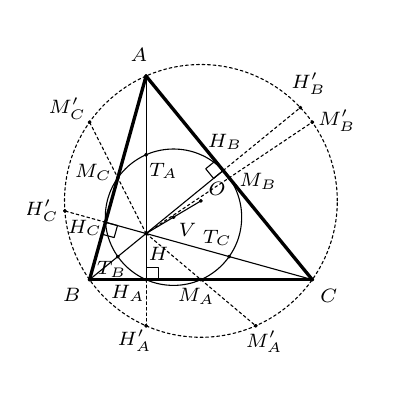
\begin{tikzpicture}[line cap=round,line join=round,>=triangle 45,x=1.0cm,y=1.0cm]
		\clip(-2.2,-2.2) rectangle (2.2,2.2);
		\draw[line width=0.4pt] (0.1834058316900359,0.5080467535662307) -- (0.0608854438221684,0.4080504889436623) -- (0.16088170844473687,0.2855301010757948) -- (0.2834020963126044,0.38552636569836324) -- cycle; 
		\draw[line width=0.4pt] (-1.2541240053078413,-0.423347573909846) -- (-1.1017402185952059,-0.46565218274715187) -- (-1.0594356097579,-0.3132683960345164) -- (-1.2118193964705355,-0.27096378719721054) -- cycle; 
		\draw[line width=0.4pt] (-0.5381658907840466,-0.9999999861642334) -- (-0.5381658903919371,-0.8418529078423136) -- (-0.696312968713857,-0.8418529074502041) -- (-0.6963129691059664,-0.9999999857721239) -- cycle; 
		\draw [line width=0.4pt,dash pattern=on 1pt off 1pt] (0.,0.) circle (1.7320508075688772cm);
		\draw [line width=1.2pt] (-0.6963129626944374,1.5859218952973992)-- (-1.4142135736923451,-0.9999999839921626);
		\draw [line width=1.2pt] (-1.4142135736923451,-0.9999999839921626)-- (1.4142135687335498,-0.9999999910049585);
		\draw [line width=1.2pt] (1.4142135687335498,-0.9999999910049585)-- (-0.6963129626944374,1.5859218952973992);
		\draw [line width=0.4pt] (0.,0.)-- (-0.6963129676532328,-0.414078079699722);
		\draw [line width=0.4pt] (-0.6963129676532328,-0.414078079699722)-- (-0.6963129626944374,1.5859218952973992);
		\draw [line width=0.4pt] (-0.6963129676532328,-0.414078079699722)-- (-0.6963129691059664,-0.9999999857721239);
		\draw [line width=0.4pt] (0.2834020963126044,0.38552636569836324)-- (-0.6963129676532328,-0.414078079699722);
		\draw [line width=0.4pt] (-0.6963129676532328,-0.414078079699722)-- (-1.4142135736923451,-0.9999999839921626);
		\draw [line width=0.4pt] (-1.2118193964705355,-0.27096378719721054)-- (-0.6963129676532328,-0.414078079699722);
		\draw [line width=0.4pt] (-0.6963129676532328,-0.414078079699722)-- (1.4142135687335498,-0.9999999910049585);
		\draw [line width=0.4pt] (-0.3481564838266164,-0.207039039849861) circle (0.8660254037844387cm);
		\draw [line width=0.4pt,dash pattern=on 1pt off 1pt] (-1.2118193964705355,-0.27096378719721054)-- (-1.727325825287838,-0.12784949469469886);
		\draw [line width=0.4pt,dash pattern=on 1pt off 1pt] (-0.6963129676532328,-0.414078079699722)-- (-1.4142135687335498,0.9999999910049585);
		\draw [line width=0.4pt,dash pattern=on 1pt off 1pt] (0.2834020963126044,0.38552636569836324)-- (1.2631171602784417,1.1851308110964485);
		\draw [line width=0.4pt,dash pattern=on 1pt off 1pt] (-0.6963129676532328,-0.414078079699722)-- (1.4142135736923451,0.9999999839921627);
		\draw [line width=0.4pt,dash pattern=on 1pt off 1pt] (-0.6963129691059664,-0.9999999857721239)-- (-0.6963129705586998,-1.5859218918445255);
		\draw [line width=0.4pt,dash pattern=on 1pt off 1pt] (-0.6963129676532328,-0.414078079699722)-- (0.6963129626944375,-1.5859218952973992);
		\begin{scriptsize}
			\draw [fill=black] (-0.6963129626944374,1.5859218952973992) circle (0.5pt);
			\draw[color=black] (-0.7860773532189839,1.855276750076106) node {$A$};
			\draw [fill=black] (-1.4142135736923451,-0.9999999839921626) circle (0.5pt);
			\draw[color=black] (-1.6404346515268833,-1.1998333795782188) node {$B$};
			\draw [fill=black] (1.4142135687335498,-0.9999999910049585) circle (0.5pt);
			\draw[color=black] (1.6249099964561875,-1.2043064544386206) node {$C$};
			\draw [fill=black] (0.,0.) circle (0.5pt);
			\draw[color=black] (0.20694526575668964,0.15103522826307858) node {$O$};
			\draw [fill=black] (-0.6963129676532328,-0.414078079699722) circle (0.5pt);
			\draw[color=black] (-0.5400582359051909,-0.6764836209112262) node {$H$};
			\draw [fill=black] (-2.479397687160656E-9,-0.9999999874985606) circle (0.5pt);
			\draw[color=black] (-0.05920268842823187,-1.2154891415896247) node {$M_A$};
			\draw [fill=black] (-0.6963129691059664,-0.9999999857721239) circle (0.5pt);
			\draw[color=black] (-0.9269792113168835,-1.1752314678460098) node {$H_A$};
			\draw [fill=black] (-0.6963129651738351,0.5859219077988387) circle (0.5pt);
			\draw[color=black] (-0.4751986504315545,0.3813985835737634) node {$T_A$};
			\draw [fill=black] (-0.3481564838266164,-0.207039039849861) circle (0.5pt);
			\draw[color=black] (-0.168793022504376,-0.36336838068311084) node {$V$};
			\draw [fill=black] (-1.0552632681933913,0.2929609556526183) circle (0.5pt);
			\draw[color=black] (-1.36534054762146,0.3635062841321568) node {$M_C$};
			\draw [fill=black] (0.35895030301955616,0.29296095214622037) circle (0.5pt);
			\draw[color=black] (0.7280584869759057,0.247206337761714) node {$M_B$};
			\draw [fill=black] (-1.2118193964705355,-0.27096378719721054) circle (0.5pt);
			\draw[color=black] (-1.4726943442674787,-0.34323954381130345) node {$H_C$};
			\draw [fill=black] (0.2834020963126044,0.38552636569836324) circle (0.5pt);
			\draw[color=black] (0.30758945011233224,0.7481907221266985) node {$H_B$};
			\draw [fill=black] (0.3589503005401585,-0.7070390353523403) circle (0.5pt);
			\draw[color=black] (0.20918180318681504,-0.46848563990254954) node {$T_C$};
			\draw [fill=black] (-1.055263270672789,-0.7070390318459423) circle (0.5pt);
			\draw[color=black] (-1.1327406548884194,-0.8665893024782961) node {$T_B$};
			\draw [fill=black] (-1.727325825287838,-0.12784949469469886) circle (0.5pt);
			\draw[color=black] (-2.0228825520783253,-0.12405887565162271) node {$H_C'$};
			\draw [fill=black] (-1.4142135687335498,0.9999999910049585) circle (0.5pt);
			\draw[color=black] (-1.6963480872800178,1.173132833864855) node {$M_C'$};
			\draw [fill=black] (1.2631171602784417,1.1851308110964485) circle (0.5pt);
			\draw[color=black] (1.3677081919917675,1.4907211489533718) node {$H_B'$};
			\draw [fill=black] (1.4142135736923451,0.9999999839921627) circle (0.5pt);
			\draw[color=black] (1.72555418081183,1.021048288611199) node {$M_B'$};
			\draw [fill=black] (-0.6963129705586998,-1.5859218918445255) circle (0.5pt);
			\draw[color=black] (-0.8419907889721187,-1.7746234991398306) node {$H_A'$};
			\draw [fill=black] (0.6963129626944375,-1.5859218952973992) circle (0.5pt);
			\draw[color=black] (0.804100759600169,-1.792515798581437) node {$M_A'$};
		\end{scriptsize}
	\end{tikzpicture}
	\caption{}\label{fig:orthocenter8}
\end{figure}

\switchcolumn
我们还可以以另一种方法理解九点圆: \par
如图\ref{fig:orthocenter8}, 连接并倍长线段$HH_{A,\ B,\ C}$与$HM_{A,\ B,\ C}$到$H_{A,\ B,\ C}'$与$M_{A,\ B,\ C}'$. 则这些点都在$\odot O$上. 同理, 如果倍长$HT_{A,\ B,\ C}$, 此时倍长后的端点就是$A$, $B$, $C$, 仍然在$\odot O$上. 所以, 我们可以说$\odot O$与$\odot V$关于$H$位似, 位似比是$2:1$. 如果有同学不了解位似是什么, 那请自行了解.


这一节, 我们对垂心的性质做了很深入的研究. 大家也可以看到, 平面几何中的内容一环套一环, 环环相扣, 变化多端. 从最开始的六组四点共圆, 到后来的相似三角形与线段乘积式和比例式, 再到垂心的对称点与顶点的对径点, 再到九点圆与欧拉线. 每一步的推导都是由上一步的结论得出的, 同时又是下一步推导的依据. 平面几何就是这样, 从很少的公理, 公设与定义出发, 通过演绎而得到一个庞大而精致的公理体系. 这样一步步搭建公理体系大厦的过程令人惊叹, 这也是平面几何独特的魅力, 是其他数学分支所几乎不能替代的.\footnote{当然, 每个人对每个数学分支的看法是不同的, 这一句的说法也在他人看来也不一定对.}\par
这一节的内容也仍然只是整个平面几何中的冰山一角, 我们只是展示了很少一部分较为简单的内容呈现给了大家. 当然, 还有更多的结构与结论, 它们更精美, 更壮观, 更精彩, 当然也更复杂. 我们在此只是“抛砖引玉”, 更多有趣的知识, 如果有兴趣, 不妨了解一下, 漫步于平面几何的浩瀚星空下, 欣赏各种漂亮精致的几何定理, 也是一件浪漫的事情.

\end{paracol}

\section{旁心与旁切圆}

\begin{paracol}{2}
本节内容在中考中几乎不会出现, 有兴趣的同学们可以了解一下.\par

\switchcolumn*
\begin{figure}[htbp]
	\centering
	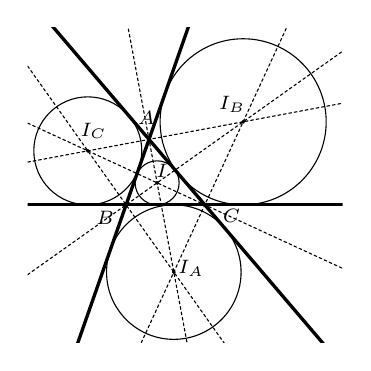
\begin{tikzpicture}[line cap=round,line join=round,>=triangle 45,x=1.0cm,y=1.0cm]
		\clip(-1.25,-1.75) rectangle (2.75,2.25);
		\draw [line width=1.2pt,domain=-1.25:2.75] plot(\x,{(-0.-0.8310235071249397*\x)/-0.29088720571092186});
		\draw [line width=1.2pt,domain=-1.25:2.75] plot(\x,{(-0.-0.*\x)/1.});
		\draw [line width=1.2pt,domain=-1.25:2.75] plot(\x,{(-0.8310235071249397--0.8310235071249397*\x)/-0.7091127942890781});
		\draw [line width=0.4pt,dash pattern=on 1pt off 1pt,domain=-1.25:2.75] plot(\x,{(-0.7634009864387107-0.18379967414772214*\x)/-0.9829637225163456});
		\draw [line width=0.4pt,dash pattern=on 1pt off 1pt,domain=-1.25:2.75] plot(\x,{(--0.4386734203766469-0.9829637225163456*\x)/0.18379967414772214});
		\draw [line width=0.4pt,dash pattern=on 1pt off 1pt,domain=-1.25:2.75] plot(\x,{(-0.-0.8155917315830882*\x)/0.5786277969241538});
		\draw [line width=0.4pt,dash pattern=on 1pt off 1pt,domain=-1.25:2.75] plot(\x,{(-0.--0.5786277969241538*\x)/0.8155917315830882});
		\draw [line width=0.4pt,dash pattern=on 1pt off 1pt,domain=-1.25:2.75] plot(\x,{(-0.9080486850579383--0.9080486850579383*\x)/0.4188646387134502});
		\draw [line width=0.4pt,dash pattern=on 1pt off 1pt,domain=-1.25:2.75] plot(\x,{(-0.4188646387134502--0.4188646387134502*\x)/-0.9080486850579383});
		\draw [line width=0.4pt] (-0.48645522891162224,0.6856719718525434) circle (0.6856719718525434cm);
		\draw [line width=0.4pt] (0.39400796500425217,0.27953196670895103) circle (0.27953196670895103cm);
		\draw [line width=0.4pt] (0.6059920349957479,-0.8541623748029623) circle (0.8541623748029623cm);
		\draw [line width=0.4pt] (1.4864552289116229,1.0545770402331476) circle (1.0545770402331476cm);
		\begin{scriptsize}
			\draw [fill=black] (0.,0.) circle (0.5pt);
			\draw[color=black] (-0.2657622109003494,-0.16197058481136473) node {$B$};
			\draw [fill=black] (0.29088720571092186,0.8310235071249397) circle (0.5pt);
			\draw[color=black] (0.25865387445478395,1.1023273046183279) node {$A$};
			\draw [fill=black] (1.,0.) circle (0.5pt);
			\draw[color=black] (1.3372543633023957,-0.13569162457853284) node {$C$};
			\draw [fill=black] (-0.48645522891162224,0.6856719718525434) circle (0.5pt);
			\draw[color=black] (-0.4135813622100287,0.9384608749384717) node {$I_C$};
			\draw [fill=black] (1.4864552289116229,1.0545770402331476) circle (0.5pt);
			\draw[color=black] (1.3471089733897075,1.2735176179070786) node {$I_B$};
			\draw [fill=black] (0.6059920349957479,-0.8541623748029623) circle (0.5pt);
			\draw[color=black] (0.825250808500238,-0.8031018001373948) node {$I_A$};
			\draw [fill=black] (0.39400796500425217,0.27953196670895103) circle (0.5pt);
			\draw[color=black] (0.45690919550252745,0.43587576048556137) node {$I$};
		\end{scriptsize}
	\end{tikzpicture}
	\caption{}\label{fig:escenter1}
\end{figure}

\switchcolumn
一个三角形有三个旁切圆, 这三个旁切圆的圆心被称为旁心, 如图\ref{fig:escenter1}所示. $ \angle A $(此处表示$ \triangle ABC $的内角, 下同)的内角平分线与$ \angle B $, $ \angle C $的外角平分线三线共点于$\triangle ABC$的$ \angle A $内的旁心$ I_A $(有时会记作$A-$旁心); $ \angle B $的内角平分线与$ \angle C $, $ \angle A $ 的外角平分线三线共点于$\triangle ABC$的$ \angle B $内的旁心$ I_B $; $ \angle C $的内角平分线与$ \angle A $, $ \angle B $的外角平分线三线共点于$\triangle ABC$的$ \angle C $内的旁心$ I_C $. 我们也顺便画出$ \triangle ABC $的内心$ I $与内切圆$ \odot I $. \par
我们罗列出旁心的性质, 由于大多数性质与内心类似, 所以略去证明. 相信大家可以独立完成这些证明.\par
首先是关于角度的结论:

\switchcolumn
\begin{figure}[htbp]
	\centering
	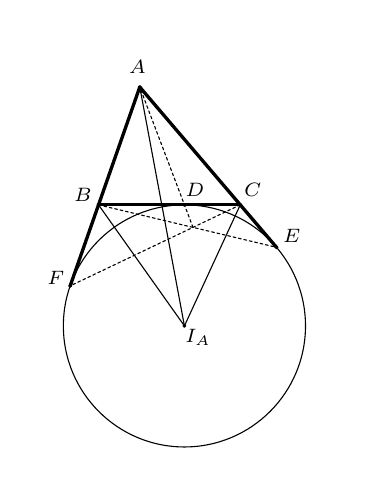
\begin{tikzpicture}[line cap=round,line join=round,>=triangle 45,x=1.8cm,y=1.8cm]
		\clip(-0.5,-1.75) rectangle (1.75,1.25);
		\draw [line width=0.4pt] (0.6059920349957479,-0.8541623748029623) circle (1.5374922746453321cm);
		\draw [line width=1.2pt] (-0.20020749414748487,-0.5719644270105201)-- (0.29088720571092186,0.8310235071249397);
		\draw [line width=1.2pt] (0.29088720571092186,0.8310235071249397)-- (1.2557524726978575,-0.29972145267852274);
		\draw [line width=1.2pt] (1.,0.)-- (0.,0.);
		\draw [line width=0.4pt] (0.29088720571092186,0.8310235071249397)-- (0.6059920349957479,-0.8541623748029623);
		\draw [line width=0.4pt] (0.6059920349957479,-0.8541623748029623)-- (0.,0.);
		\draw [line width=0.4pt] (0.6059920349957479,-0.8541623748029623)-- (1.,0.);
		\draw [line width=0.4pt,dash pattern=on 1pt off 1pt] (1.,0.)-- (-0.20020749414748487,-0.5719644270105201);
		\draw [line width=0.4pt,dash pattern=on 1pt off 1pt] (0.,0.)-- (1.2557524726978575,-0.29972145267852274);
		\draw [line width=0.4pt,dash pattern=on 1pt off 1pt] (0.6662924695859103,-0.15902986554667858)-- (0.29088720571092186,0.8310235071249397);
		\begin{scriptsize}
			\draw [fill=black] (0.,0.) circle (0.5pt);
			\draw[color=black] (-0.10928844430414293,0.07228503954280929) node {$B$};
			\draw [fill=black] (0.29088720571092186,0.8310235071249397) circle (0.5pt);
			\draw[color=black] (0.2747341779624978,0.9739033700818797) node {$A$};
			\draw [fill=black] (1.,0.) circle (0.5pt);
			\draw[color=black] (1.088695170810269,0.10567831104425633) node {$C$};
			\draw [fill=black] (0.6059920349957479,-0.8541623748029623) circle (0.5pt);
			\draw[color=black] (0.7025854690747878,-0.9357743439071236) node {$I_A$};
			\draw [fill=black] (0.6059920349957479,0.) circle (0.5pt);
			\draw[color=black] (0.679627594917543,0.10567831104425633) node {$D$};
			\draw [fill=black] (-0.20020749414748487,-0.5719644270105201) circle (0.5pt);
			\draw[color=black] (-0.30129975543746335,-0.516271370670195) node {$F$};
			\draw [fill=black] (1.2557524726978575,-0.29972145267852274) circle (0.5pt);
			\draw[color=black] (1.364189660697207,-0.2199060860948524) node {$E$};
		\end{scriptsize}
	\end{tikzpicture}
	\caption{}\label{fig:escenter2}
\end{figure}

\switchcolumn
\begin{theorem}
	\kaishu 如图\ref{fig:escenter2}, $ \triangle ABC $的$ \angle A $中的旁心为$ I_A $, 我们有$ \angle AI_AB=\angle BCA/2 $, $ \angle AI_AC=\angle ABC/2 $, $ \angle BI_AC=90^\circ-\angle BAC/2 $. 对于余下两个旁心有完全类似的结论.
\end{theorem}\par

还有关于线段长的结论: 
\begin{theorem}
	\kaishu 如图\ref{fig:escenter2}, 设$ BC=a $, $ CA=b $, $ AB=c $, 半周长$ p=(a+b+c)/2 $. 则有如下结论:
	\begin{align*}
		AE=AF&=\frac{a+b+c}{2}=p;\\
		BF=BD&=\frac{a+b-c}{2}=p-c;\\
		CD=CE&=\frac{a-b+c}{2}=p-b.
	\end{align*}
\end{theorem}

由此, 结合塞瓦定理, 我们可以得到以下结论:
\begin{theorem}
	\kaishu 如图\ref{fig:escenter2}, 三条直线$ AD $, $ BE $, $ CF $共点.
\end{theorem}

对于旁心, 我们也有鸡爪定理: 

\switchcolumn*
\begin{figure}[htbp]
	\centering
	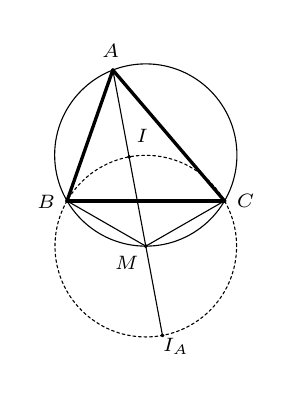
\begin{tikzpicture}[line cap=round,line join=round,>=triangle 45,x=2.0cm,y=2.0cm]
		\clip(-0.25,-1.1) rectangle (1.25,1.1);
		\draw [line width=1.2pt] (1.,0.)-- (0.,0.);
		\draw [line width=0.4pt] (0.5,0.29140465099791996) circle (1.1574397100898508cm);
		\draw [line width=1.2pt] (0.29088720571092186,0.8310235071249397)-- (0.,0.);
		\draw [line width=1.2pt] (1.,0.)-- (0.29088720571092186,0.8310235071249397);
		\draw [line width=0.4pt] (0.6059920349957479,-0.8541623748029623)-- (0.29088720571092186,0.8310235071249397);
		\draw [line width=0.4pt] (0.5,-0.28731520404700545)-- (0.,0.);
		\draw [line width=0.4pt] (0.5,-0.28731520404700545)-- (1.,0.);
		\draw [line width=0.4pt,dash pattern=on 1pt off 1pt] (0.5,-0.28731520404700545) circle (1.153343013117212cm);
		\begin{scriptsize}
			\draw [fill=black] (0.,0.) circle (0.5pt);
			\draw[color=black] (-0.13237065728962527,-0.005598636785663996) node {$B$};
			\draw [fill=black] (0.29088720571092186,0.8310235071249397) circle (0.5pt);
			\draw[color=black] (0.276406083642755,0.952912341952332) node {$A$};
			\draw [fill=black] (1.,0.) circle (0.5pt);
			\draw[color=black] (1.132722877147655,0.001449238057997737) node {$C$};
			\draw [fill=black] (0.6059920349957479,-0.8541623748029623) circle (0.5pt);
			\draw[color=black] (0.6904687307078816,-0.923584335172605) node {$I_A$};
			\draw [fill=black] (0.39400796500425217,0.27953196670895103) circle (0.5pt);
			\draw[color=black] (0.4772705166871143,0.4102259789903784) node {$I$};
			\draw [fill=black] (0.5,-0.28731520404700545) circle (0.5pt);
			\draw[color=black] (0.3786002688758501,-0.39323175318705944) node {$M$};
		\end{scriptsize}
	\end{tikzpicture}
	\caption{}\label{fig:escenter3}
\end{figure}

\switchcolumn

\begin{theorem}
	\kaishu 
	如图\ref{fig:escenter3}, $ \angle BAC $的内角平分线交$ \triangle ABC $的外接圆于另一点$ M $, 则
	\[ MI=MB=MI_A=MC. \]
\end{theorem}\par
这便是鸡爪定理的完整形式. 因为由四条线段$ MI $, $ MI_A $, $ MB $, $ MC $所构成的图形形似鸡爪, 故称为“鸡爪定理”.\par
如果将内心与旁心、内切圆与旁切圆结合起来, 还有其他有趣的性质.\par

\setcounter{figure}{22}
\begin{figure}[thbp]
	\centering
	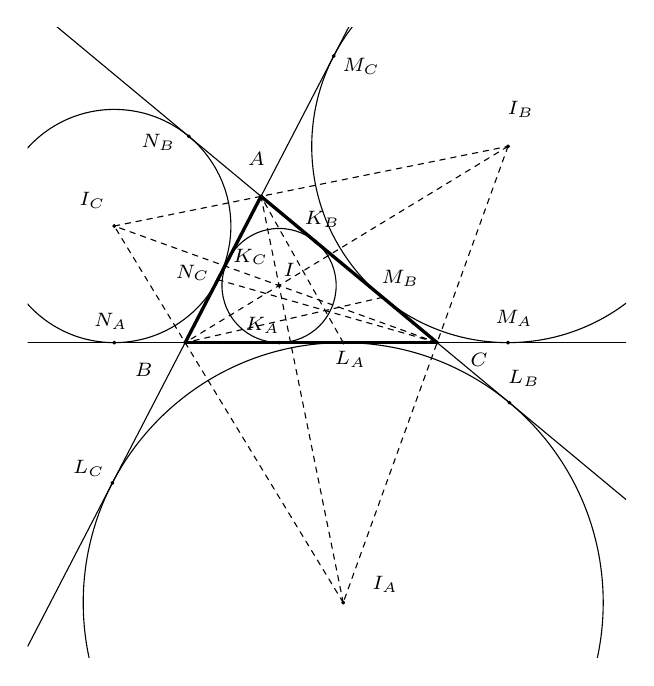
\begin{tikzpicture}[line cap=round,line join=round,>=triangle 45,x=1.6cm,y=1.6cm]
		\clip(-1.25,-2.5) rectangle (3.5,2.5);
		\draw [line width=0.4pt,domain=-1.25:3.5] plot(\x,{(-0.-1.1613169631436235*\x)/-0.6020794705093755});
		\draw [line width=0.4pt,domain=-1.25:3.5] plot(\x,{(-0.-0.*\x)/2.});
		\draw [line width=0.4pt,domain=-1.25:3.5] plot(\x,{(-2.322633926287247--1.1613169631436235*\x)/-1.3979205294906245});
		\draw [line width=0.4pt] (-0.5627416690423479,0.9256252355087863) circle (0.9256252355087863);
		\draw [line width=0.4pt] (0.7453702442487048,0.45315412675893607) circle (0.45315412675893607);
		\draw [line width=0.4pt] (1.2546297557512953,-2.063676864590298) circle (2.063676864590298);
		\draw [line width=0.4pt] (2.5627416690423486,1.5580404129415875) circle (1.5580404129415875);
		\draw [line width=1.2pt] (2.,0.)-- (0.,0.);
		\draw [line width=1.2pt] (0.6020794705093755,1.1613169631436235)-- (0.,0.);
		\draw [line width=1.2pt] (2.,0.)-- (0.6020794705093755,1.1613169631436235);
		\draw [line width=0.4pt,dash pattern=on 2pt off 2pt] (-0.5627416690423479,0.9256252355087863)-- (2.5627416690423486,1.5580404129415875);
		\draw [line width=0.4pt,dash pattern=on 2pt off 2pt] (2.5627416690423486,1.5580404129415875)-- (1.2546297557512953,-2.063676864590298);
		\draw [line width=0.4pt,dash pattern=on 2pt off 2pt] (1.2546297557512953,-2.063676864590298)-- (-0.5627416690423479,0.9256252355087863);
		\draw [line width=0.4pt,dash pattern=on 2pt off 2pt] (1.2546297557512953,-2.063676864590298)-- (0.6020794705093755,1.1613169631436235);
		\draw [line width=0.4pt,dash pattern=on 2pt off 2pt] (2.5627416690423486,1.5580404129415875)-- (0.,0.);
		\draw [line width=0.4pt,dash pattern=on 2pt off 2pt] (2.,0.)-- (-0.5627416690423479,0.9256252355087863);
		\draw [line width=0.4pt,dash pattern=on 2pt off 2pt] (1.2546297557512953,0.)-- (0.6020794705093755,1.1613169631436235);
		\draw [line width=0.4pt,dash pattern=on 2pt off 2pt] (1.567139594459377,0.3595970736696483)-- (0.,0.);
		\draw [line width=0.4pt,dash pattern=on 2pt off 2pt] (0.25901087107918813,0.49959138777541734)-- (2.,0.);
		\begin{scriptsize}
			\draw [fill=black] (0.,0.) circle (0.5pt);
			\draw[color=black] (-0.3284826703585897,-0.213324713354675319) node {$B$};
			\draw [fill=black] (0.6020794705093755,1.1613169631436235) circle (0.5pt);
			\draw[color=black] (0.5667504774024771,1.4586451738293886) node {$A$};
			\draw [fill=black] (2.,0.) circle (0.5pt);
			\draw[color=black] (2.3313927398161183,-0.1338913087176529193) node {$C$};
			\draw [fill=black] (-0.5627416690423479,0.9256252355087863) circle (0.5pt);
			\draw[color=black] (-0.7373631945763846,1.12723674893707) node {$I_C$};
			\draw [fill=black] (2.5627416690423486,1.5580404129415875) circle (0.5pt);
			\draw[color=black] (2.662801164708436,1.8503096759748556) node {$I_B$};
			\draw [fill=black] (1.2546297557512953,-2.063676864590298) circle (0.5pt);
			\draw[color=black] (1.5867997851879234,-1.919999157865027) node {$I_A$};
			\draw [fill=black] (0.7453702442487048,0.45315412675893607) circle (0.5pt);
			\draw[color=black] (0.8266388747043848,0.5755722467916027) node {$I$};
			\draw [fill=black] (0.7453702442487048,0.) circle (0.5pt);
			\draw[color=black] (0.6140945381013796,0.1350436563568226) node {$K_A$};
			\draw [fill=black] (0.25901087107918813,0.49959138777541734) circle (0.5pt);
			\draw[color=black] (0.06011430064709223,0.5535400646948948) node {$N_C$};
			\draw [fill=black] (0.34306859943018725,0.661725575368206) circle (0.5pt);
			\draw[color=black] (0.5194064167035746,0.6812682412735206) node {$K_C$};
			\draw [fill=black] (1.0349398760499988,0.8017198894739753) circle (0.5pt);
			\draw[color=black] (1.0875351450904054,0.9767245944307723) node {$K_B$};
			\draw [fill=black] (1.567139594459377,0.3595970736696483) circle (0.5pt);
			\draw[color=black] (1.707311939694221,0.5118919984779101) node {$M_B$};
			\draw [fill=black] (0.028741322736408424,1.6376153667937274) circle (0.5pt);
			\draw[color=black] (-0.21227452137037428,1.5920693448899321) node {$N_B$};
			\draw [fill=black] (1.1795429209626205,2.2751534805047613) circle (0.5pt);
			\draw[color=black] (1.3974235423923131,2.1946301174214202) node {$M_C$};
			\draw [fill=black] (-0.5627416690423479,0.) circle (0.5pt);
			\draw[color=black] (-0.5910270069615948,0.16808371153764314) node {$N_A$};
			\draw [fill=black] (-0.5774634504532448,-1.1138365173611375) circle (0.5pt);
			\draw[color=black] (-0.7648352939018615,-0.9956458445614972) node {$L_C$};
			\draw [fill=black] (2.573338147772967,-0.47629840365010323) circle (0.5pt);
			\draw[color=black] (2.6886251978169287,-0.28282899477686028) node {$L_B$};
			\draw [fill=black] (1.2546297557512953,0.) circle (0.5pt);
			\draw[color=black] (1.311343432030672,-0.1351008181982344) node {$L_A$};
			\draw [fill=black] (2.5627416690423486,0.) circle (0.5pt);
			\draw[color=black] (2.6111530984914517,0.1922596784291508) node {$M_A$};
		\end{scriptsize}
	\end{tikzpicture}
	\caption{}\label{fig:escenter4}
\end{figure}

如图\ref{fig:escenter4}, 如果我们考虑各个切线长, 我们会得到以下结论:

\begin{theorem}
	\kaishu 如图\ref{fig:escenter4}, 设$ BC=a $, $ CA=b $, $ AB=c $, 半周长$ p=(a+b+c)/2 $. $ \odot I $切$ BC $, $ CA $, $ AB $于$ K_A $, $ K_B $,$ K_C $; $ \odot I_A $切$ BC $, $ CA $, $ AB $于$ L_A $, $ L_B $,$ L_C $; $ \odot I_B $切$ BC $, $ CA $, $ AB $于$ M_A $, $ M_B $,$ M_C $; $ \odot I_C $切$ BC $, $ CA $, $ AB $于$ N_A $, $ N_B $,$ N_C $. 则:
	\[ N_AB=M_AC=p-a,\ N_AC=M_AB=p, \]
	即, $ N_A $与$ M_A $关于$ BC $中点对称; 
	\[ K_AB=L_AC=p-b,\ K_AC=L_AB=p-c, \]
	即, $ K_A $与$ L_A $关于$ BC $中点对称.
	\[ N_BA=L_BC=p-b,\ N_BC=L_BA=p, \]
	即, $ N_B $与$ L_B $关于$ AC $中点对称;
	\[ K_BA=M_BC=p-a,\ K_BC=M_BA=p-c, \]
	即, $ K_B $与$ M_B $关于$ AC $中点对称.
	\[ M_CA=L_CB=p-c,\ M_CB=L_CA=p, \]
	即, $ M_C $与$ L_C $关于$ AB $中点对称;
	\[ K_CA=N_CB=p-a,\ K_CB=N_CA=p-b, \]
	即, $ K_C $与$ N_C $关于$ AB $中点对称.
\end{theorem}

我们还能注意到, 由于一个角的内外角平分线垂直, 所以
\[AI_A\perp I_BI_C,\ BI_B\perp I_CI_A,\ CI_C\perp I_AI_B.\]
所以, $ I $, $ I_A $, $ I_B $, $ I_C $构成一个垂心组, 之前垂心的结论在这里都适用.\par
所以我们可以看到, 三个旁心和一个内心组成的结构和之前提到的垂心的结构相呼应. $ \triangle ABC $就是$ \triangle I_AIBI_C $的垂足三角形, 之前提到的“垂心是垂足三角形的内心”的结论在这里也是显然的.\par
并且, $ \triangle ABC $的外接圆就是$ \triangle I_AI_BI_C $的九点圆(因为$ \triangle ABC $是$ \triangle I_AIBI_C $的垂足三角形, 而一个三角形的九点圆过三个垂足, 即为垂足三角形的外接圆), 所以$ \triangle ABC $的外接圆过$ II_A $, $ II_B $, $ II_C $的中点, 这与之前提到的鸡爪定理也是吻合的.\par
如果考虑塞瓦定理, 还可以得到如下定理:
\begin{theorem}
	\kaishu 在一个三角形中, 一个顶点与对边上这个顶点所对应的内角内的旁切圆的切点连成线段, 共有三条这样的线段, 此三线共点. 即, 如图\ref{fig:escenter4}, $ AL_A $, $ BM_B $, $ CN_C $共点.
\end{theorem}
并且, 由切线长的结论, 我们会发现
\[ AB+BL_A=AC+CL_A=p, \]
即$ AL_A $平分$ \triangle ABC $的周长. 同理, $ BM_B $, $ CN_C $都平分$ \triangle ABC $的周长.
\end{paracol}

\chapter{若干特殊几何结构}
\thispagestyle{empty}
\setcounter{figure}{-1}


这一章, 我们会列出若干特殊的几何结构与经典模型. 这些内容大多都是考试中经常出现的, 所以希望大家能够对这些结构很熟悉, 这样才能在考试中熟练运用, 在短时间内发现问题的本质, 并熟练运用脑海中对应的知识解题. \par


\section{一组临边相等的圆内接四边形}

\begin{paracol}{2}

\switchcolumn
\stepcounter{figure}
\begin{figure}[htbp]
	\centering
	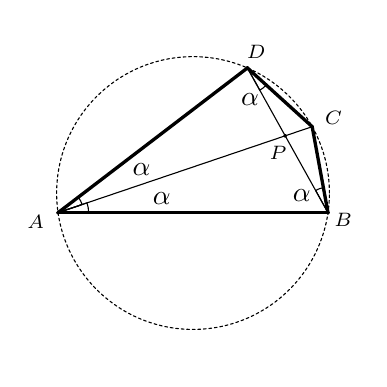
\begin{tikzpicture}[line cap=round,line join=round,>=triangle 45,x=1.0cm,y=1.0cm]
		\clip(-2.1,-2.1) rectangle (2.1,2.1);
		\draw [shift={(-1.7139987311678728,-0.2494160170376431)},line width=0.4pt] (0,0) -- (18.694515820428173:0.323250321073206) arc (18.694515820428173:37.38903164085635:0.323250321073206) -- cycle;
		\draw [shift={(-1.7139987311678728,-0.2494160170376431)},line width=0.4pt] (0,0) -- (0.:0.3879003852878472) arc (0.:18.694515820428173:0.3879003852878472) -- cycle;
		\draw [shift={(0.6906906798049193,1.588378539527218)},line width=0.4pt] (0,0) -- (-60.89036748193636:0.323250321073206) arc (-60.89036748193636:-42.19585166150819:0.323250321073206) -- cycle;
		\draw [shift={(1.7139987311678728,-0.2494160170376431)},line width=0.4pt] (0,0) -- (100.41511669763547:0.323250321073206) arc (100.41511669763547:119.10963251806365:0.323250321073206) -- cycle;
		\draw [line width=0.4pt,dash pattern=on 1pt off 1pt] (0.,0.) circle (1.7320508075688772cm);
		\draw [line width=1.2pt] (-1.7139987311678728,-0.2494160170376431)-- (1.7139987311678728,-0.2494160170376431);
		\draw [line width=1.2pt] (-1.7139987311678728,-0.2494160170376431)-- (0.6906906798049193,1.588378539527218);
		\draw [line width=1.2pt] (0.6906906798049193,1.588378539527218)-- (1.5132762467064722,0.842612011043026);
		\draw [line width=1.2pt] (1.5132762467064722,0.842612011043026)-- (1.7139987311678728,-0.2494160170376431);
		\draw [line width=0.4pt] (1.7139987311678728,-0.2494160170376431)-- (0.6906906798049193,1.588378539527218);
		\draw [line width=0.4pt] (1.5132762467064722,0.842612011043026)-- (-1.7139987311678728,-0.2494160170376431);
		\draw (1.1452050847899065,0.162804165625869) node[anchor=north west] {$\alpha$};
		\draw (0.4857744298005661,1.391155385704053) node[anchor=north west] {$\alpha$};
		\draw (-0.8912719379712915,0.4925194931205395) node[anchor=north west] {$\alpha$};
		\draw (-0.6326716811127266,0.12401412709708423) node[anchor=north west] {$\alpha$};
		\begin{scriptsize}
			\draw [fill=black] (-1.7139987311678728,-0.2494160170376431) circle (0.5pt);
			\draw[color=black] (-1.9967880360416561,-0.36409385772345737) node {$A$};
			\draw [fill=black] (1.7139987311678728,-0.2494160170376431) circle (0.5pt);
			\draw[color=black] (1.9080758425226725,-0.3382338320376009) node {$B$};
			\draw [fill=black] (0.6906906798049193,1.588378539527218) circle (0.5pt);
			\draw[color=black] (0.802559744452308,1.7952182870455613) node {$D$};
			\draw [fill=black] (1.5132762467064722,0.842612011043026) circle (0.5pt);
			\draw[color=black] (1.7852407205148544,0.9483024458337604) node {$C$};
			\draw [fill=black] (1.1705220476950517,0.7266326802983794) circle (0.5pt);
			\draw[color=black] (1.0805550205752652,0.5086820091741998) node {$P$};
		\end{scriptsize}
	\end{tikzpicture}
	\caption{}\label{3.1.1}
\end{figure}

\switchcolumn
如图, 圆内接四边形$ABCD$中, $CB=CD$, 则会有以下结论: 
\begin{theorem}
	\kaishu 
	\textbf{1. }$AD$平分$\angle CAB$;\\
	\textbf{2. }$\angle DAC=\angle BAC=\angle CDB=\angle CBD$;\\
	\textbf{3. }$\triangle DCP\sim\triangle ACD$, $\triangle BCP\sim\triangle ACB$; $\triangle ADP\sim\triangle ACB$, $\triangle ABP\sim\triangle ACD$;\\
	\textbf{4. }$CD^2=CB^2=CP\cdot CA$, $AP\cdot AC=AD\cdot AB=AC^2-BC^2$;\\
	\textbf{5. }$AP^2=AD\cdot AB-DP\cdot BP$(注意, 这条性质与点$C$无关, 所以这相当于一个计算三角形角平分线长的公式);\\
	\textbf{6. }$AB+AD=2AC\cos{\alpha}$.
\end{theorem}

\switchcolumn
\begin{figure}[H]
	\centering
	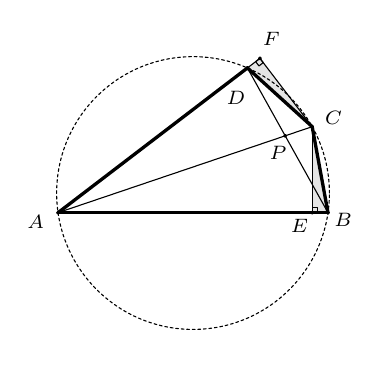
\begin{tikzpicture}[line cap=round,line join=round,>=triangle 45,x=1.0cm,y=1.0cm]
		\clip(-2.1,-2.1) rectangle (2.1,2.1);
		\fill[line width=2.pt,fill=black,fill opacity=0.10000000149011612] (0.6906906798049193,1.588378539527218) -- (0.850170891689229,1.7102619993800345) -- (1.5132762467064722,0.842612011043026) -- cycle;
		\fill[line width=2.pt,fill=black,fill opacity=0.10000000149011612] (1.5132762467064722,0.842612011043026) -- (1.5132762467064722,-0.2494160170376431) -- (1.7139987311678728,-0.2494160170376431) -- cycle;
		\draw[line width=0.4pt] (0.795688520349386,1.6686236052405587) -- (0.8373269144888618,1.6141412339007157) -- (0.8918092858287048,1.6557796280401915) -- (0.850170891689229,1.7102619993800345) -- cycle; 
		\draw[line width=0.4pt] (1.58184799492195,-0.2494160170376431) -- (1.58184799492195,-0.1808442688221653) -- (1.5132762467064722,-0.1808442688221653) -- (1.5132762467064722,-0.2494160170376431) -- cycle; 
		\draw [line width=0.4pt,dash pattern=on 1pt off 1pt] (0.,0.) circle (1.7320508075688772cm);
		\draw [line width=1.2pt] (-1.7139987311678728,-0.2494160170376431)-- (1.7139987311678728,-0.2494160170376431);
		\draw [line width=1.2pt] (-1.7139987311678728,-0.2494160170376431)-- (0.6906906798049193,1.588378539527218);
		\draw [line width=1.2pt] (0.6906906798049193,1.588378539527218)-- (1.5132762467064722,0.842612011043026);
		\draw [line width=1.2pt] (1.5132762467064722,0.842612011043026)-- (1.7139987311678728,-0.2494160170376431);
		\draw [line width=0.4pt] (1.7139987311678728,-0.2494160170376431)-- (0.6906906798049193,1.588378539527218);
		\draw [line width=0.4pt] (1.5132762467064722,0.842612011043026)-- (-1.7139987311678728,-0.2494160170376431);
		\draw [line width=0.4pt] (0.6906906798049193,1.588378539527218)-- (0.850170891689229,1.7102619993800345);
		\draw [line width=0.4pt] (0.850170891689229,1.7102619993800345)-- (1.5132762467064722,0.842612011043026);
		\draw [line width=0.4pt] (1.5132762467064722,0.842612011043026)-- (1.5132762467064722,-0.2494160170376431);
		\begin{scriptsize}
			\draw [fill=black] (-1.7139987311678728,-0.2494160170376431) circle (0.5pt);
			\draw[color=black] (-1.9967880360416566,-0.3640938577234566) node {$A$};
			\draw [fill=black] (1.7139987311678728,-0.2494160170376431) circle (0.5pt);
			\draw[color=black] (1.9080758425226716,-0.3382338320376001) node {$B$};
			\draw [fill=black] (0.6906906798049193,1.588378539527218) circle (0.5pt);
			\draw[color=black] (0.5439594875937424,1.206902702692326) node {$D$};
			\draw [fill=black] (1.5132762467064722,0.842612011043026) circle (0.5pt);
			\draw[color=black] (1.7852407205148533,0.9483024458337611) node {$C$};
			\draw [fill=black] (1.1705220476950517,0.7266326802983794) circle (0.5pt);
			\draw[color=black] (1.0805550205752643,0.5086820091742005) node {$P$};
			\draw [fill=black] (0.850170891689229,1.7102619993800345) circle (0.5pt);
			\draw[color=black] (0.9965099370962307,1.9633084540036287) node {$F$};
			\draw [fill=black] (1.5132762467064722,-0.2494160170376431) circle (0.5pt);
			\draw[color=black] (1.3520852902767573,-0.4222789155166337) node {$E$};
		\end{scriptsize}
	\end{tikzpicture}
	\caption{}\label{3.2.2}
\end{figure}

\switchcolumn
如图\ref{3.2.2}, 若过$C$作$AB$, $AD$的垂线$DE$, $DF$, 则有
$\mathrm{Rt}\triangle CFD\cong\mathrm{Rt}\triangle CEB.$\par
以上所罗列的五条性质, 前三条都不困难, 我们重点说明后三条.事实上, 如图\ref{3.1.1}由$\triangle DCP\sim\triangle ACD$, 有
\[\frac{DC}{AC}=\frac{CP}{CD}, \]
即
\[DC^2=AC\cdot CP.\]
又$DC=BC$, 所以
\[CD^2=CB^2=CP\cdot CA.\]
这样就证明了第一个式子. \par
至于第二个式子, 由$\triangle ADP\sim\triangle ACB$, 有
\[\frac{AD}{AC}=\frac{AP}{AB},\]
即
\[AP\cdot AC=AD\cdot AB.\]
如图\ref{3.2.2}, 在$\mathrm{Rt}\triangle ACE$与$\mathrm{Rt}\triangle BCE$中运用勾股定理, 有
\[AC^2-AE^2=CE^2=BC^2-BE^2,\]
即
\[AC^2-BC^2=AE^2-BE^2.\]
又熟知$\triangle CAF\cong\triangle CAE$, 所以$AE=AF$. 又$DF=BE$, 所以,
\begin{align*}
	AE^2-BE^2&=(AE-BE)(AE+BE)=(AF-DF)(AE+AB)\\
	&=AD\cdot AB.
\end{align*}
结合$AC^2-BC^2=AE^2-BE^2$, 即得
\[AC^2-BC^2=AB\cdot AD.\]\par
下面我们证明第五条性质. 由第四条性质, 有
\[AP\cdot AC=AB\cdot AD.\]
又由相交弦定理, 有
\[AP\cdot PC=DP\cdot BP.\]
两式相减, 即得
\begin{align*}
	&AB\cdot AD-DP\cdot BP=AP\cdot AC-AP\cdot PC\\
	=&AP(AC-PC)=AP^2.
\end{align*}\par
下面证明第六个式子. 事实上, 因为$AE=AF$, $BE=DF$, 所以
\begin{align*}
	AB+AD&=(AF-DF)+(AE+EB)=2AE\\
	&=2AC\cos{\alpha.}
\end{align*}
还有一种基于托勒密定理的证明方法: 在圆内接四边形$ABCD$中考虑托勒密定理, 得到
\[AB\cdot CD+AD\cdot CB=AC\cdot BD.\]
又有$CB=CD$, 所以可以将上式改写为
\[AB+AD=AC\cdot\frac{BD}{BC}.\]
而在$\triangle BCD$中考虑正弦定理, 有
\[\frac{CB}{\sin{\angle CDB}}=\frac{BD}{\sin{\angle BCD}},\]
即
\begin{align*}
	\frac{BD}{BC}&=\frac{\sin{\angle BCD}}{\sin{\angle CDB}}=\frac{\left(180^\circ-2\alpha\right)}{\sin{\alpha}}\\
	&=\frac{\sin{2\alpha}}{\sin{\alpha}}=\frac{2\sin{\alpha}\cos{\alpha}}{\sin{\alpha}}\\
	&=2\cos{\alpha}.
\end{align*}
结合前文所述, 即得
\[AB+AD=AC\cdot 2\cos{\alpha}\]
\[\]




\end{paracol}

\end{document}